%DIF PREAMBLE EXTENSION ADDED BY LATEXDIFF
%DIF UNDERLINE PREAMBLE %DIF PREAMBLE
\RequirePackage[normalem]{ulem} %DIF PREAMBLE
\RequirePackage{color}\definecolor{RED}{rgb}{1,0,0}\definecolor{BLUE}{rgb}{0,0,1} %DIF PREAMBLE
\providecommand{\DIFadd}[1]{{\protect\color{blue}\uwave{#1}}} %DIF PREAMBLE
\providecommand{\DIFdel}[1]{{\protect\color{red}\sout{#1}}}                      %DIF PREAMBLE
%DIF SAFE PREAMBLE %DIF PREAMBLE
\providecommand{\DIFaddbegin}{} %DIF PREAMBLE
\providecommand{\DIFaddend}{} %DIF PREAMBLE
\providecommand{\DIFdelbegin}{} %DIF PREAMBLE
\providecommand{\DIFdelend}{} %DIF PREAMBLE
%DIF FLOATSAFE PREAMBLE %DIF PREAMBLE
\providecommand{\DIFaddFL}[1]{\DIFadd{#1}} %DIF PREAMBLE
\providecommand{\DIFdelFL}[1]{\DIFdel{#1}} %DIF PREAMBLE
\providecommand{\DIFaddbeginFL}{} %DIF PREAMBLE
\providecommand{\DIFaddendFL}{} %DIF PREAMBLE
\providecommand{\DIFdelbeginFL}{} %DIF PREAMBLE
\providecommand{\DIFdelendFL}{} %DIF PREAMBLE
%DIF END PREAMBLE EXTENSION ADDED BY LATEXDIFF

\documentclass[master=cws,masteroption=gs,dutch]{kulemt}
\setup{title={Automatische verificatie en kwaliteitscontrole van UML-diagrammen met FO(.)},
	author={Thomas Vochten},
	promotor={Prof. dr. Marc Denecker},
	assessor={TBD},
	assistant={Matthias van der Hallen}}

%\setup{coverpageonly}
\setup{font=lm}

\setup{filingcard,
	translatedtitle={TBD},
	udc=TBD,
	shortabstract={\lipsum[2]}}

\usepackage[pdfusetitle,colorlinks,plainpages=false]{hyperref}
\usepackage{float}
\usepackage{todonotes}
\usepackage{amsmath}
\usepackage{amssymb}
\usepackage{listings}
\usepackage{svg}
\svgsetup{clean=true}
\usepackage{relsize}
\usepackage{pdflscape}
\usepackage{subcaption}

\lstset{
	basicstyle=\scriptsize\ttfamily,
	commentstyle=\ttfamily\color{gray},
	numbers=left,
	numberstyle=\ttfamily\color{gray}\footnotesize,
	stepnumber=1,
	numbersep=5pt,
	backgroundcolor=\color{white},
	showspaces=false,
	showstringspaces=false,
	showtabs=false,
	frame=single,
	tabsize=2,
	captionpos=b,
	breaklines=true,
	breakatwhitespace=false,
	title=\lstname,
	escapeinside={},
	keywordstyle={},
	morekeywords={}
}

\IfFileExists{lipsum.sty}%
{\usepackage{lipsum}\setlipsumdefault{11-13}}%
{\newcommand{\lipsum}[1][11-13]{\par And some text: lipsum ##1.\par}}

\newcommand{\parbreak}{\vspace{5mm}}

\begin{document}
	
\begin{preface}
	\lipsum[1]
\end{preface}

\tableofcontents*

\begin{abstract}
	\lipsum[1]
\end{abstract}

\mainmatter

\chapter{Inleiding}

\section{Situering}\label{sec:situering}

UML\cite{RumbaughJames2005Tuml} is een visuele modelleertaal geschikt voor algemene doeleinden. Men gebruikt het om artefacten van een softwaresysteem te specificeren en te visualiseren. Deze artefacten bekijken een softwaresysteem vanuit verscheidene oogpunten, en het is de ambitie van UML om genoeg soorten artefacten aan te bieden om een volledige beschrijving te geven van een softwaresysteem. Met behulp van deze artefacten kan men een softwaresysteem ontwerpen en begrijpen.

Wanneer tijdens het modelleerproces het aantal artefacten toeneemt en als individuele artefacten complex worden, wordt het echter moeilijk om een overzicht te behouden van de structuur van het systeem en hoe de componenten van het systeem zich gedragen. Het kan dat men moeilijk die structuur en dat gedrag begrijpt. Tijdens het modelleren kunnen er ook beslissingen worden genomen die ervoor zorgen dat het systeem onmogelijk kan werken als het wordt ge\"implementeerd zoals beschreven in de artefacten. Een beslissing kan er ook toe leiden dat een systeem ongewenst gedrag vertoont. Daarom bekijken we in deze masterproef of we voor enkele soorten artefacten, met name klassediagrammen en sequentiediagrammen, gereedschap kunnen aanbieden die de modelleerder helpt om beter inzicht te verkrijgen in wat hij modelleert.

Voor klassediagrammen willen we nagaan:

\begin{itemize}
	\item Of de structuur van een klassediagram niet zo is dat het eigenlijk onmogelijk is om te implementeren.
	\item Of een klassediagram redundante informatie bevat of op zulk een manier gestructureerd is die het moeilijker maakt om het diagram te begrijpen.
\end{itemize}

Voor sequentiediagrammen willen we nagaan:

\begin{itemize}
	\item Of we het gedrag beschreven in sequentiediagrammen kunnen simuleren.
	\item Of we automatisch kunnen controleren of dat gedrag beantwoordt aan bepaalde functionele eisen op het softwaresysteem.
\end{itemize} 

We bouwen zulk een gereedschap op door klassediagrammen en sequentiediagrammen te representeren in FO($\cdot$), een uitbreiding van eerste-orde-predicatenlogica.

Sectie \ref{sec:uml-artifacts} geeft een overzicht van de artefacten die UML aanbiedt. Sectie \ref{sec:intro-idp} geeft een inleiding tot IDP\cite{DeCatBroes2014PLaa}, een kennisbanksysteem voor FO($\cdot$). Sectie \ref{sec:research-q} overloopt de probleemstellingen die we bekijken in deze masterproef. Sectie \ref{sec:text-structure} geeft het verdere verloop van deze tekst en beschrijft de bijdragen geleverd in deze masterproef.

\section{Overzicht van UML-artefacten}\label{sec:uml-artifacts}

James Rumbaugh et al.\cite{RumbaughJames2005Tuml} geven een informele indeling van de soorten artefacten in vier domeinen: Het structureel domein, het dynamisch domein, het fysisch domein en het domein van het modelbeheer. De volgende subsecties geven een kort overzicht van elk domein.

\subsection{Structureel domein}

Artefacten in het structureel domein bekijken het softwaresysteem vanuit de volgende oogpunten:

\begin{itemize}
	\item Het statisch oogpunt: Hieronder vallen klassediagrammen. Klasses zijn modelelementen die discrete stukken informatie bevatten in de vorm van attributen. Ze defini\"eren ook bewerkingen die erop uitgevoerd kunnen worden en er wordt ook gespecificeerd met welke andere klasses ze in verband staan door middel van associaties.
	\item Het ontwerpoogpunt: Hieronder vallen interne structuurdiagrammen, collaboratiediagrammen en componentdiagrammen.
	\begin{itemize}
		\item Interne structuurdiagrammen beschrijven voor een bepaalde klasse gedefinieerd in een klassediagram de interne structuur in meer detail.
		\item Collaboratiediagrammen geven weer hoe individuele objecten kunnen samenwerken om een deel van de functionaliteit van de software te bewerkstelligen.
		\item Componentdiagrammen handelen over componenten. Componenten stellen modulaire delen van een systeem voor die extern zichtbare stukken hebben. Deze stukken zijn ofwel functionaliteit die de component aanbiedt gelabeld met een naam, genaamd \textit{interfaces}, ofwel een poort gelabeld met de naam van een \textit{interface}. Een poort kan verbonden worden met een corresponderende \textit{interface} van een andere component. Componentdiagrammen geven weer hoe componenten met elkaar worden verbonden om op hoog niveau het gedrag van een deel van het systeem te specificeren.
	\end{itemize}
	\item Het \textit{use case} oogpunt: Hieronden vallen \textit{use case} diagrammen. Deze diagrammen benoemen verscheidene actoren, die concrete personen of externe systemen kunnen zijn, en geven grafisch weer welke actoren een rol spelen bij welke \textit{use cases}. De ontwerper geeft elders een tekstuele beschrijving voor elke \textit{use case}. Een \textit{use case} beschrijft een concrete dienst die een systeem aanbiedt en benoemt de relevante actoren.
\end{itemize}

Aangezien deze masterproef onder andere handelt over klassediagrammen, geven we hier een klein voorbeeld. Beschouw volgend klassediagram:

\begin{figure}[H]
	\label{fig:cd}
	\centering
	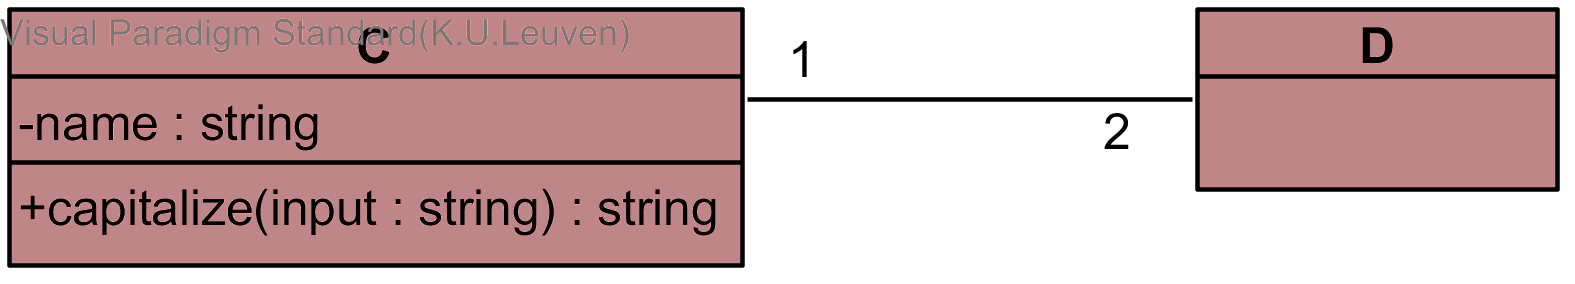
\includegraphics{intro/cd.png}
	\caption{Een voorbeeld van een klassediagram}
\end{figure}

Dit klassediagram drukt uit dat er twee klasses bestaan: \textit{C} en \textit{D}. \textit{C} heeft \'e\'en attribuut, \textit{name}, dat van type \textit{string} is. \textit{D} heeft ook \'e\'en attribuut, \textit{number}, van type \textit{int}. \textit{C} heeft ook \'e\'en operatie \textit{getDNumber} dat \textit{index}, van type \textit{int}, als parameter heeft. \textit{getDNumber(int)} geeft een resultaat terug dat ook van type \textit{int} is. Voorts drukt de lijn tussen \textit{C} en \textit{D} uit dat er een relatie bestaat tussen de twee klasses. Beschouw klasse C. Als we vanuit die klasse de lijn volgen, zien we dat er aan het ander uiteinde staat dat elke \textit{C}-object in relatie moet staan tot exact twee \textit{D}-objecten. Zo ook zien we dat, als we vertrekken vanuit \textit{D}, elk \textit{D}-object in relatie moet staan tot exact \'e\'en \textit{C}-object.

\subsection{Dynamisch domein}

Artefacten in het dynamisch domein bekijken het softwaresysteem vanuit de volgende oogpunten:

\begin{itemize}
	\item Het toestandsautomaatoogpunt: Hieronder vallen toestandsautomaatdiagrammen. Deze diagrammen benoemen toestanden waarin het systeem zich kan bevinden en de mogelijke overgangen tussen de toestanden.
	\item Het activiteitsoogpunt: Hieronder vallen activiteitsdiagrammen. Deze diagrammen beschrijven hoe de besturingsstroom van het systeem kan verlopen tussen activiteiten. Activiteiten zijn processen die bestaan in het systeem.
	\item Het interactieoogpunt: Hieronder vallen sequentiediagrammen en communicatiediagrammen.
	\begin{itemize}
		\item Sequentiediagrammen beschrijven een tijdverloop van een interactie tussen objecten die instanties zijn van klasses gedefinieerd in een klassediagram. Deze diagrammen beschrijven hoe de toestand van \'e\'en of meerdere objecten verandert ten gevolge van een oproep van een methode gedefinieerd voor de klasse waar een bepaald object een instantie van is. Indien de operatie een resultaat heeft, wordt ook getoond hoe het resultaat wordt berekend.
		\item Communicatiediagrammen zijn gelijkaardig aan sequentiediagrammen, maar in plaats van het tijdverloop centraal te stellen tonen ze expliciet hoe de objecten betrokken in een oproep met elkaar in verband staan. 
	\end{itemize}
\end{itemize}

Aangezien sequentiediagrammen het tweede soort diagram zijn dat we beschouwen in deze masterproef, geven we ook daar een klein voorbeeld van. Beschouw volgend sequentiediagram:

\begin{figure}[H]
	\label{fig:sd}
	\centering
	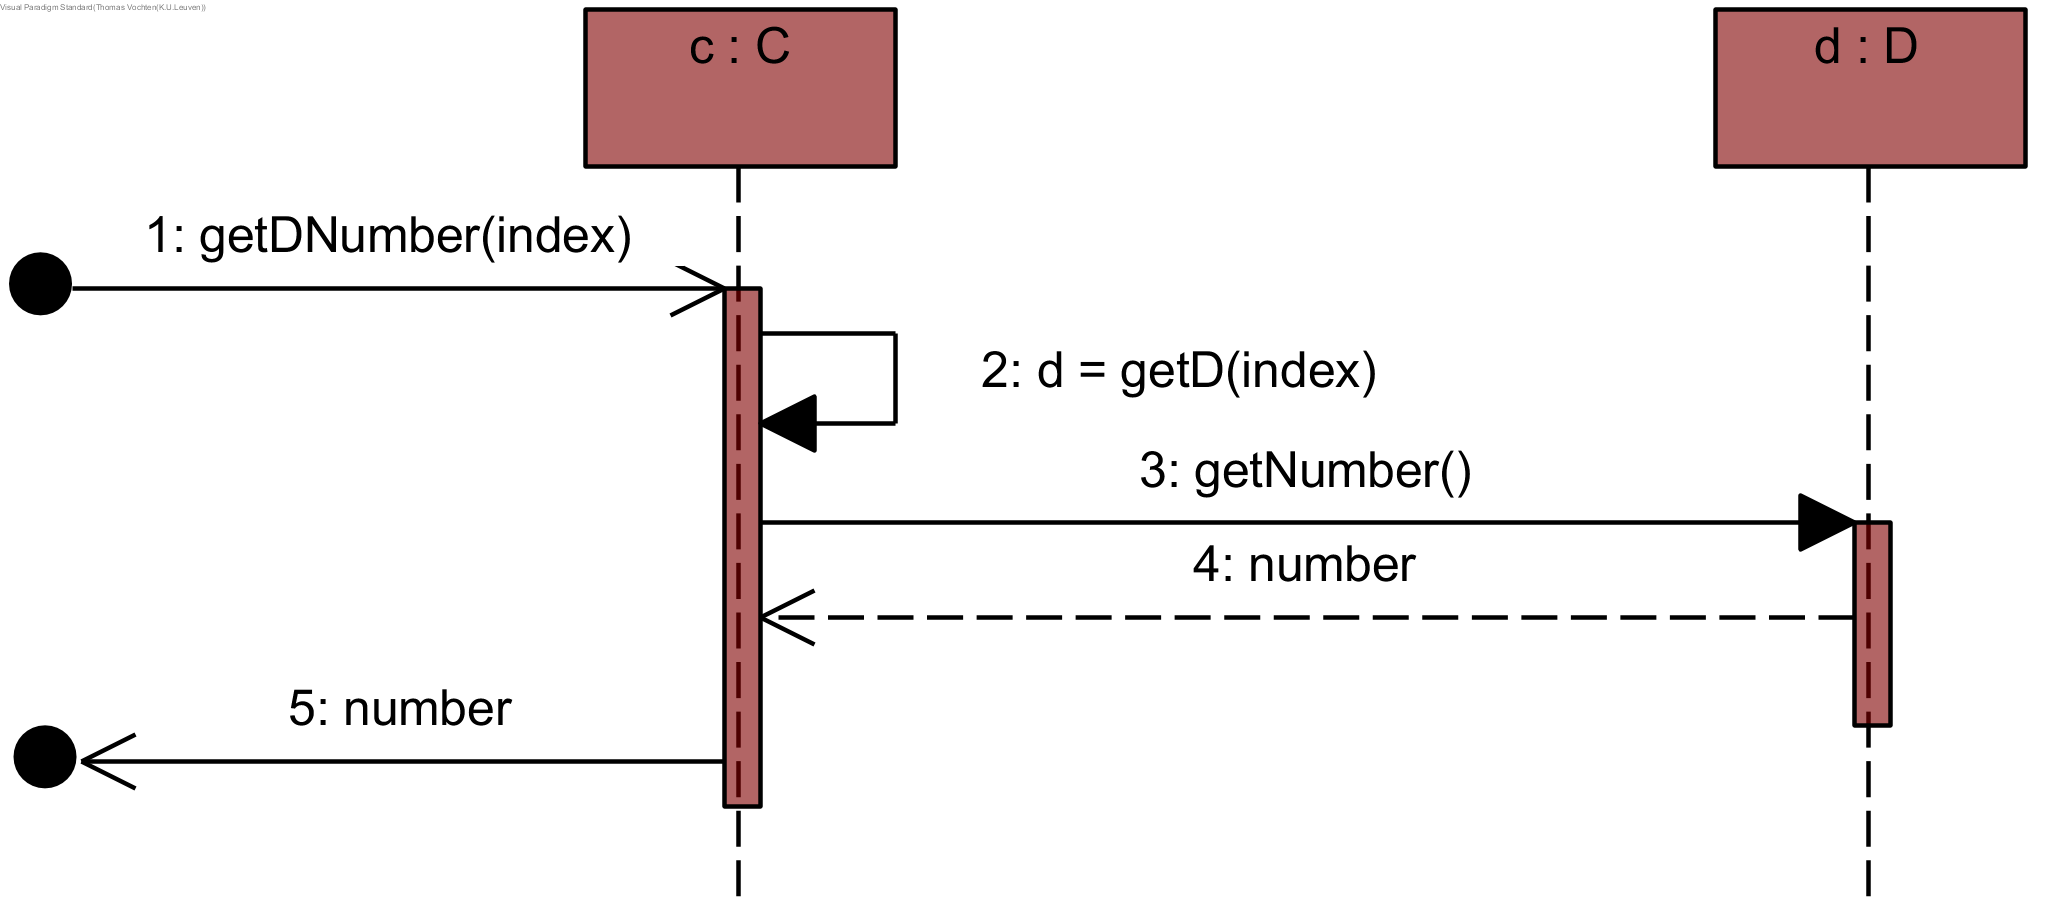
\includegraphics{intro/sd.png}
	\caption{Een voorbeeld van een sequentiediagram}
\end{figure}

Het toont hoe de juiste instantie van \textit{D} wordt opgehaald op basis van invoervariabele \textit{index} en hoe de waarde van het attribuut \textit{number} wordt doorgegeven aan instantie \textit{c}. \textit{c} geeft dan \textit{number} door als uitvoer van het sequentiediagram. Hoofdstuk \ref{sec:gedrag} legt meer in detail uit wat de betekenis is van de elementen die kunnen voorkomen in een sequentiediagram.

\subsection{Fysisch domein}

Artefacten in het fysisch domein bekijken het softwaresysteem vanuit het oogpunt van \textit{deployment}. \textit{Deployment} diagrammen geven weer hoe het systeem fysisch ge\"implementeerd wordt. Deze diagrammen benoemen fysische machines, geven aan welke verbindingen er bestaan tussen die machines en tonen welke concrete softwareartefacten draaien op elke machine.

\subsection{Modelbeheerdomein}

In dit domein beoogt men het beheer van de modellering van het systeem zelf. Tot dit domein behoren de \textit{package} diagrammen. Dit soort diagrammen organiseert de verscheidene soorten modelelementen van het softwaresysteem zoals klasses en \textit{use cases} in \textit{packages}. Een \textit{package} kan ook andere \textit{packages} bevatten. \textit{Package} diagrammen tonen welke \textit{packages} afhankelijk zijn van welke andere \textit{packages}. Zo krijgt men dus een beeld van welke modellen gebruik maken van elementen gedefinieerd in een ander model in hun beschrijving.

\section{Het kennisbanksysteem IDP}\label{sec:intro-idp}

Kennisbanksystemen\cite{1999XKSS} beogen het modelleren van kennis over een probleemdomein op een gestructureerde manier in een kennisbank. Ze bieden inferentiemethodes aan waarmee geredeneerd kan worden op die kennis. Zo kan een kennisbanksysteem nieuwe, meer precieze kennis afleiden. Ze laten ook het oplossen van concrete instanties van een probleem binnen het probleemdomein toe.

In deze masterproef gebruiken we IDP\cite{DeCatBroes2014PLaa}. In IDP zijn kennisbanken opgesteld in FO($\cdot$), een uitbreiding van predicatenlogica.

IDP bouwt verder op eerder werk in het onderzoeksdomein van het logisch programmeren. Het ondersteunt constructies gebaseerd op logisch programmeren, in het bijzonder inductieve definities, maar breekt ook met enkele fundamentele idee\"en uit dat paradigma. Logische theorie\"en opgesteld in FO($\cdot$) zijn geen uitvoerbare programma's---ze zijn beschrijvingen van kennis in het beschouwde probleemdomein. In IDP bestaat de fundamentele oplossingsstrategie voor problemen in een toepassingsdomein uit het specificeren van informatie over het domein in logica. De gebruiker past dan een vorm van inferentie toe om een antwoord te krijgen op concrete vragen geformuleerd in termen van het toepassingsdomein.

Bij het opstellen van logische theorie\"en ondersteunt IDP alle concepten uit de klassieke eerste-orde-predicatenlogica: Constanten, variabelen, predicaten, functies en existenti\"ele en universele kwantoren. IDP ondersteunt ook concepten die eerste-orde-predicantelogica uitbreiden. Concreet gaat het over de volgende vier concepten:

\begin{itemize}
	\item \textbf{Logische types}: Alle variabelen gebruikt in een logische zin hebben een type. Dit betekent ook dat alle argumenten van een predicaat en functie en het resultaat van een functie een type hebben.
	\item \textbf{Aggregaten}: Dit zijn de functies \textit{cardinaliteit}, \textit{som}, \textit{product}, \textit{minimum} en \textit{maximum}. De ontwerper specificeert \'e\'en variabele of een tupel van variabelen. Hij bindt die variabele of tupel dan in een logische zin. Als de ontwerper \'e\'en variabele specificeert, worden alle waarden die voldoen aan de logische zin als argument doorgegeven aan de aggregaatfunctie. Als de ontwerper een tupel specificeert, dan wordt voor elke tupel die voldoet aan de zin het eerste element doorgegeven aan de aggregaatfunctie.
	\item \textbf{Inductieve definities}: Dit is een mechanisme om de interpretatie van een predicaat of functie te defini\"eren analoog aan hoe een concept kan gedefinieerd worden in een recursieve definitie in de wiskunde of in verscheidene domeinen van de wetenschap.
	\item \textbf{Parti\"ele functies}: IDP laat toe om een functie te specificeren als \textit{partieel}. Dit betekent dat niet alle elementen van het domein noodzakelijk worden afgebeeld op een element uit het codomein.
\end{itemize}

De inferentievormen die IDP ondersteunt zijn: Modelexpansie gegeven een deels ingevulde structuur; bepalen of een structuur een model is voor een theorie en/of bepalen of een structuur kan uitgebreid worden tot een model voor de theorie; het vinden van optimale modellen gegeven een aggregate term; propagatie, wat gegeven een structuur en een theorie een preciezere structuur geeft die alle oplossingen behoudt; \textit{query}-inferentie, wat alle objecten die beantwoorden aan een bepaalde \textit{query} ophaalt uit een gegeven structuur; deductie; en \textit{theorem proving} door middel van de functie \textit{entails(theory, theory)}.

De basisblokken van een specificatie in IDP zijn als volgt:

\begin{itemize}
	\item \textbf{Vocabularium}: Hier specificeert de ontwerper de logische types die bestaan in het beschouwd domein en de predicaten en functies over die logische types.
	\item \textbf{Theorie}: Hier schrijft de ontwerper zinnen in FO($\cdot$) die bepalen welke structuren over het beschouwde vocabularium modellen zijn. Indien de ontwerper een inconsistente theorie ontwerpt, zullen er geen modellen zijn.
	\item \textbf{Structuur}: De ontwerper vult hier de logische types gedefinieerd in het vocabularium in. \textit{Constructed types} hebben geen invulling nodig aangezien ze al volledig worden gespecificeerd in het vocabularium. De ontwerper kan ook voor \'e\'en of meerdere predicaten aangeven welke tupels wel of geen lid zijn. Hij kan ook voor \'e\'en of meerdere functies specificeren welke elementen uit het domein afgebeeld worden op welk element uit het codomein.
\end{itemize}

De ontwerper kan meerdere vocabularia, theorie\"en en structuren neerschrijven. Elke theorie en structuur kan wel maar de symbolen van \'e\'en vocabularium gebruiken.

Broes De Cat et al.\cite{DeCatBroes2014PLaa} geven een uitgebreidere inleiding tot IDP.

\section{Probleemstellingen}\label{sec:research-q}

Zoals aangehaald in sectie \ref{sec:situering}, kunnen er inconsistenties of onduidelijkheden sluipen in een klassediagram. Het kan ook dat het gedrag gemodelleerd in een sequentiediagram ingaat tegen bepaalde functionele eisen op het softwaresysteem.

\subsection{Probleemstellingen omtrent klassediagrammen}

We beschouwen twee categorie\"en van gebreken in een klassediagram:

\begin{itemize}
	\item \textbf{Inconsistenties:} Het klassediagram is zo opgebouwd dat geen enkele mogelijke toestand van de software kan beantwoorden aan de voorwaarden die worden opgelegd. Dit betekent dat het stuk van de software dat wordt beschreven in het diagram onmogelijk kan werken.
	\item \textbf{Kwaliteitsgebreken:} Deze gebreken hebben een negatieve impact op de kwaliteit van het softwareontwerp. Zo kunnen ze bijvoorbeeld onduidelijkheden in het ontwerp introduceren of het onderhoud van de software \'e\'enmaal ingezet in productie bemoeilijken.
\end{itemize}

We onderzoeken hoe we klassediagrammen kunnen vertalen naar een voorstelling die ons toelaat om automatisch de consistentie van het diagram te controleren en om bepaalde soorten kwaliteitsgebreken op te sporen.

\subsection{Probleemstellingen omtrent sequentiediagrammen}

We willen het volgende uitvoeren voor sequentiediagrammen:

\begin{itemize}
	\item Het simuleren van het gedrag gemodelleerd in een bepaald stel sequentiediagrammen.
	\item Het verifi\"eren of de uitvoer van een sequentiediagram beantwoordt aan de vereisten opgelegd op de methode die dat sequentiediagram modelleert.
	\item Het verifi\"eren of het gedrag gemodelleerd in een stel sequentiediagrammen overeenkomt met gewenst gedrag in het beoogd softwaresysteem. Een voorbeeld van gewenst gedrag is dat een speler in een schaakspel maar \'e\'en stuk van zijn kleur mag bewegen per beurt.
\end{itemize}

We onderzoeken hoe we sequentiediagrammen kunnen vertalen naar een voorstelling die een uitvoering van het systeem kan simuleren. Met die voorstelling verifi\"eren we ook de uitvoer en het gedrag van sequentiediagrammen.

\section{Verdere verloop van deze tekst}\label{sec:text-structure}

Hoofdstuk \ref{sec:literatuur} geeft een overzicht van literatuur omtrent het gebruik van logica om klassediagrammen en bepaalde soorten dynamische diagrammen voor te stellen.

Hoofdstuk \ref{sec:consistentie} beschrijft hoe we FO($\cdot$) gebruiken om klassediagrammen voor te stellen. We tonen aan dat we consistentie van een klassediagram kunnen verifi\"eren, maar dat er verder onderzoek is vereist om inconsistentie te kunnen controleren.

Hoofdstuk \ref{sec:kwaliteitsgebrek} beschrijft een alternatieve voorstellingswijze die we gebruiken om bepaalde kwaliteitsgebreken op te sporen. We tonen aan dat we de aanwezigheid van losstaande klasses, \textit{many-to-many} associaties en onvoldoende nauw gespecificeerde bovengrenzen op een uiteinde van een associatie kunnen detecteren.

In hoofdstuk \ref{sec:gedrag} beschrijven we hoe sequentiediagrammen voor te stellen in lineaire tijdscalculus\cite{BogaertsBart2014Sdsu}, een methode om in FO($\cdot$) dynamische systemen te modelleren.

In hoofdstuk \ref{sec:evaluatie} evalueren we ons vertalingsproces. We modelleren een spel in een klassediagram en een stel sequentiediagrammen. Die diagrammen gebruiken we enerzijds voor een simulatie van het spel en anderzijds om verificaties van gewenste eigenschappen uit te voeren. Daarbij letten we op rekentijd en geheugengebruik. We tonen aan dat we het spel Nim kunnen modelleren in een klassediagram en een stel sequentiediagrammen en dat we met de theorie opgesteld volgens de regels beschreven in hoofdstukken \ref{sec:consistentie} en \ref{sec:gedrag} het verloop van een spel kunnen simuleren. We nemen waar dat er relatief veel tijd en geheugen nodig is om deze simulaties uit te voeren. Verder tonen we aan dat we kunnen verifi\"eren of de uitvoer van een sequentiediagram voldoet aan bepaalde eisen op de methode gemodelleerd in dat sequentiediagram. Als laatste tonen we aan dat we kunnen controleren of de sequentiediagrammen garanderen dat een spelbeurt altijd verloopt zoals voorgeschreven door de spelregels van Nim.

Hoofdstuk \ref{sec:decl-seq} geeft een aanzet om de ontwerptaal beschikbaar voor sequentiediagrammen uit te breiden met declaratieve constructies. Het doel is om ervoor te zorgen dat er significant minder berichten nodig zijn in een sequentiediagram om het gedrag van een methode te specificeren. We modelleren Nim opnieuw met deze constructies en tonen aan dat er significant minder rekentijd en geheugen nodig is om het gedrag in het bekomen sequentiediagram te simuleren.

Hoofdstuk \ref{sec:conclusie} geeft een besluit en geeft een aanzet tot verder onderzoek.
\chapter{Relevante literatuur}
In de literatuur kan men verscheidene methoden om UML-diagrammen te vertalen naar logica onderscheiden. Het gaat voornamelijk over klassediagrammen, terwijl sommige werken ook sequentiediagrammen en toestandsdiagrammen beschouwen. De logica waarnaar vertaald wordt is vaak eerste-orde-predikatenlogica, maar een aantal onderzoekers verkiezen talen die behoren tot de klasse van de description logics of relationele logica.

In deze sectie bespreken we een aantal van deze werken.

\section{Redeneren op UML-klassediagrammen gebruikmakend van description logics}
In \cite{BerardiDaniela2005RoUc} toont men eerst een methode om een klassediagram automatisch te vertalen naar eerste-orde logica.

Voor elke klasse definieert men een unair predicaat dat lidmaatschap van die klasse uitdrukt. Vervolgens definieert men voor alle attributen van een klasse een predikaat dat een object van die klasse in verband brengt met een waarde voor dat attribuut. Elke methode krijgt ook een predikaat dat voor combinaties van object waar de methode voor wordt opgeroepen en een stel van parameterwaarden een resultaat definieert. In de uitvoertheorie voegt men dan voorwaarden toe waaraan beantwoord moet worden. Een object heeft zoveel verschillende waardes voor een bepaald attribuut als opgelegd door het diagram. Voor attribuutwaarden, parameterwaarden en resultaatwaarden wordt afgedwongen dat ze van het juiste type zijn. Een bepaalde combinatie van oproepobject en parameterwaarden moet ook een uniek resultaat hebben bij een oproep.

Associaties krijgen een predikaat dat objecten van de betrokken klasses in verband brengt. De uitvoertheorie dwingt af dat de objecten van het juiste type zijn en dat er gehoorzaamd wordt aan de gespecificeerde multipliciteiten.

Om overerving te modelleren, stelt de uitvoertheorie dat als een object een lid is van een subklasse, dat het dan ook een lid is van de superklasse. Voor een subklasse $C_1$ van superklasse $C$ wordt dit uitgedrukt als $\forall{x}(C_1(x) \Rightarrow C(x)$. Merk op dat deze aanpak niet uitsluit dat een object een lid kan zijn van twee klasses die niet in verband staan met elkaar in een overervingshi\"erarchie, zelfs als de ontwerper dit niet wenst.

De paper stelt een aantal redeneertaken voor die mogelijk zouden moeten zijn voor deze modelleringsmethode. Allereerst is er controle op consistentie van het gehele diagram, wat wil zeggen of er minstens \'e\'en model bestaat van het diagram waarvan de interpretatie voor minstens \'e\'en klasse een object bevat. Verder is er klasseconsistentie, namelijk of voor een klasse een model bestaat waarvoor de interpretatie van die klasse niet leeg is; klassesubsumptie, wat betekent dat het diagram impliceert dat de ene klasse een subklasse is van een andere klasse; klasse\"equivalentie, wat betekent het diagram oplegt dat voor twee klasses de interpretatie dezelfde is in alle modellen en dat \'e\'en van die klasses dus uit het diagram kan worden gehaald; en het detecteren van eigenschappen van klasses en associaties die maken dat bepaalde gespecificeerde multipliciteiten en typering in het diagram eigenlijk strenger zijn dan expliciet neergeschreven in het diagram.

De rest van de paper handelt over description logics \todo{Nederlandstalige term?}. Men geeft een beschrijving van de talen $\mathcal{DLR}_{ifd}$, $\mathcal{ALCQI}$ en $\mathcal{ALC}$, beschrijft hoe men een klassediagram kan vertalen naar $\mathcal{DLR}_{ifd}$ en geeft men een gevalstudie van software die een specificatie van een klassediagram vertaalt naar een beschrijving in $\mathcal{ALCQI}$ en kan antwoorden op queries zoals of een object van een bepaalde klasse exact eenmaal deelneemt aan een bepaalde associatie zonder dat het diagram dit expliciet oplegt. Men concludeert dat dit soort van redeneertaak behoort tot de klasse van EXPTIME-harde problemen.

De methode om klassediagrammen te vertalen naar eerste-orde-predikatenlogica voorgesteld in deze paper dient als inspiratie voor onze eigen methode gepresenteerd in hoofdstuk \ref{sec:consistentie}. We passen deze methode aan om gebruik te maken van constructies aangeboden door FO(.)\cite{DeCatBroes2014PLaa}.

\section{Het modelleren van klassediagrammen en OCL-constraints in relationele logica}
In \cite{KuhlmannMirco2012FUaO} geeft men een inleiding tot relationele logica en de semantiek ervan. Men beschrijft hoe een instantie van een model van relationele logica wordt opgebouwd door relaties die atomen of tupels van atomen bevatten en welke operaties op relaties beschikbaar zijn. Relationele logica biedt relationele bewerkingen zoals joins, cartesisch product en transitieve sluiting aan. Verder kan men ook gebruikmaken van verzamelingcomprehensie, bewerkingen op verzamelingen zoals unie en deelverzameling, booleaanse operatoren zoals conjunctie en implicatie, universele en existenti\"ele kwantoren en bewerkingen op gehele getallen. In de paper vertaalt men klassediagrammen en OCL-constraints\cite{WarmerJosB1999Ocl:} \todo{Nederlandstalige term?} op zulk een manier dat er rechtstreeks gebruik wordt gemaakt van de structuur aangeboden door relationele logica. Op die manier bekomt men modellen die op een effici\"ente manier verwerkt kunnen worden ten koste van significante beperkingen op diagrammen en OCL-constraints die kunnen dienen als invoer.

Men schetst hoe primitive types voorgesteld worden door unaire relaties van atomen. In relationele logica worden objecten voorgesteld door constanten, en deze constanten worden gebruikt als atomen in binaire relaties die objecten verbinden met waarden voor klasseattributen. Eveneens brengt men objecten in verband met elkaar in relaties die associaties voorstellen. Er worden voorwaarden gelegd op relaties die attributen en associaties voorstellen zodanig dat de gebruikte objecten van het juiste type zijn en dat de multipliciteiten gespecificeerd in het diagram afgedwongen worden. Aangezien men relaties op zulk een eenvoudige wijze gebruikt, is het eenvoudig om een stel van relaties en type- en multipliciteitsvoorwaarden te vertalen naar een klassediagram.

Men beschrijft hoe uitdrukkingen in OCL vertaald kunnen worden naar relationele logica. Bewerkingen op booleaanse waarden, gehele getallen, het allesomvattende type OclAny\cite{WarmerJosB1999Ocl:}, bewerkingen op verzamelingen met \textit{collect} in het bijzonder en navigatie van associaties worden ondersteund.

De auteurs gebruiken Kodkod\cite{10.1007/978-3-540-71209-1_49} om geldige instanties van een relationeel model te berekenen. Kodkod vertaalt relationele modellen naar SAT-formules en vertaalt oplossingen naar instanties van dat relationeel model.

\section{Klassediagrammen en activiteitsdiagrammen modelleren met \textit{Concurrent Transaction Frame Logic}}

In \cite{RamalhoFranklin2004CTFL} vertaalt men klassediagrammen en activiteitsdiagrammen\cite{RumbaughJames2005Tuml} naar uitvoerbare programma's in Concurrent Transaction Frame Logic\cite{kifer1995deductive,kifer1996concurrency} (CTFL). CTFL is een integratie van twee uitbreidingen van eerste-orde Horn-logica: Frame Logic (FL), wat objecten en overerving kan modelleren; en Concurrent Transaction Logic (CTL), wat gedrag betreffende simultane logische databank updates, transacties, procescommunicatie en tijdsgebonden randvoorwaarden betreffende uitvoering modelleert.

FL biedt een syntaxis aan waarmee men een klasse kan defini\"eren. Men specificeert een klassenaam, een klasse die dient als superklasse, een lijst van attributen met hun type en een lijst van methodes met parameters en hun type en een resultaattype. Objectcreatie wordt ook aangeboden, waarbij men de ge\"instantieerde klasse moet opgeven en ook attribuutwaarden en combinaties van argumenten en resultaat voor methodes. Deze twee soorten termen noemt men \textit{F-Molecules}. Binnen \textit{F-Molecules} worden logische variabelen ondersteund in alle mogelijke velden van klassedefinitie of objectinstantiatie. De auteurs tonen hoe klasses, associaties en overerving eenvoudig kunnen worden gemodelleerd met deze F-Molecules.

CTL breidt Horn-logica uit met vijf nieuwe connectieven: Seri\"ele conjunctie, seri\"ele disjunctie, concurrente conjunctie, concurrente disjunctie en atomische modaliteit. Deze laatste voorkomt gedeeltelijke uitvoering van een formule. Als de uitvoering wordt onderbroken of faalt, moet de toestand van alle betrokken variabelen en objecten teruggebracht zoals die was v\'o\'or de uitvoering van de formule begon. CTL definieert ook enkele bewerkingen die atomische veranderingen en synchronisatie voor hun rekening nemen. De auteurs tonen hoe de verscheidene elementen van een activiteitsdiagram, zijnde \textit{action states}, \textit{activity states}, \textit{fork} en \textit{join pairs}, \textit{synch states} en vertakkingen binnen een activiteitsdiagram gemodelleerd kunnen worden met behulp van CTFL-termen en deze vijf connectieven. Vervolgens wordt getoond hoe de genoemde klasses, attributen en methodes in een activiteitsdiagram in verband worden gebracht met hun definities in het klassediagram.

Het resultaat van deze vertaling is een uitvoerbaar programma in CTFL waarmee men de consistentie van het ontwerp in het klassediagram en de activiteitsdiagrammen kan controleren.

\parbreak

In het voorgaande merken we dat de literatuur zich voornamelijk toelegt op het vertalen van UML-diagrammen naar talen die een deelverzameling zijn van eerste-orde-predikatenlogica. Op deze manier wordt er ingeboet aan expressiviteit ten voordele van rekentijd en ruimtegebruik. We denken echter aan het modelleren van overerving: Het bepalen van tot welke klasses een object behoort ten gevolge van de gespecificeerde klassehi\"erarchie\"en is een voorbeeld van het berekenen van een transitieve sluiting, wat niet uit te drukken is in eerste-orde-predikatenlogica en dus ook niet in deze deelverzamelingen. \todo{citeer bewijs hiervan?} We merken ook op dat het ontbreekt aan een simulatiemethode voor sequentiediagrammen. In deze masterproef richten we ons op sequentiediagrammen in plaats van activiteitsdiagrammen omdat voorgaande bovenop het modelleren van interacties tussen objecten ook toelaten om variabelen te defini\"eren.
\section{Controleren van consistentie}\label{sec:consistentie}
In dit hoofdstuk treden we meer in detail over hoe we de consistentie van een diagram willen controleren. Daarvoor willen we een specifieke vorm van logische theorie automatisch laten genereren. In deze theorie\"en staan \textbf{objecten} centraal. Deze objecten zijn instanties van een klasse die voorkomt in het beschouwde diagram, hebben exact de attributen en operaties van die klasse en maken deel uit van exact die relaties die het diagram voorschrijft voor die klasse. Aan de hand van volgend voorbeeld zullen we illustreren welke regels we gebruiken om zulk een theorie op te bouwen:

\begin{figure}[H]
	\label{fig:diagram-voorbeeld}
	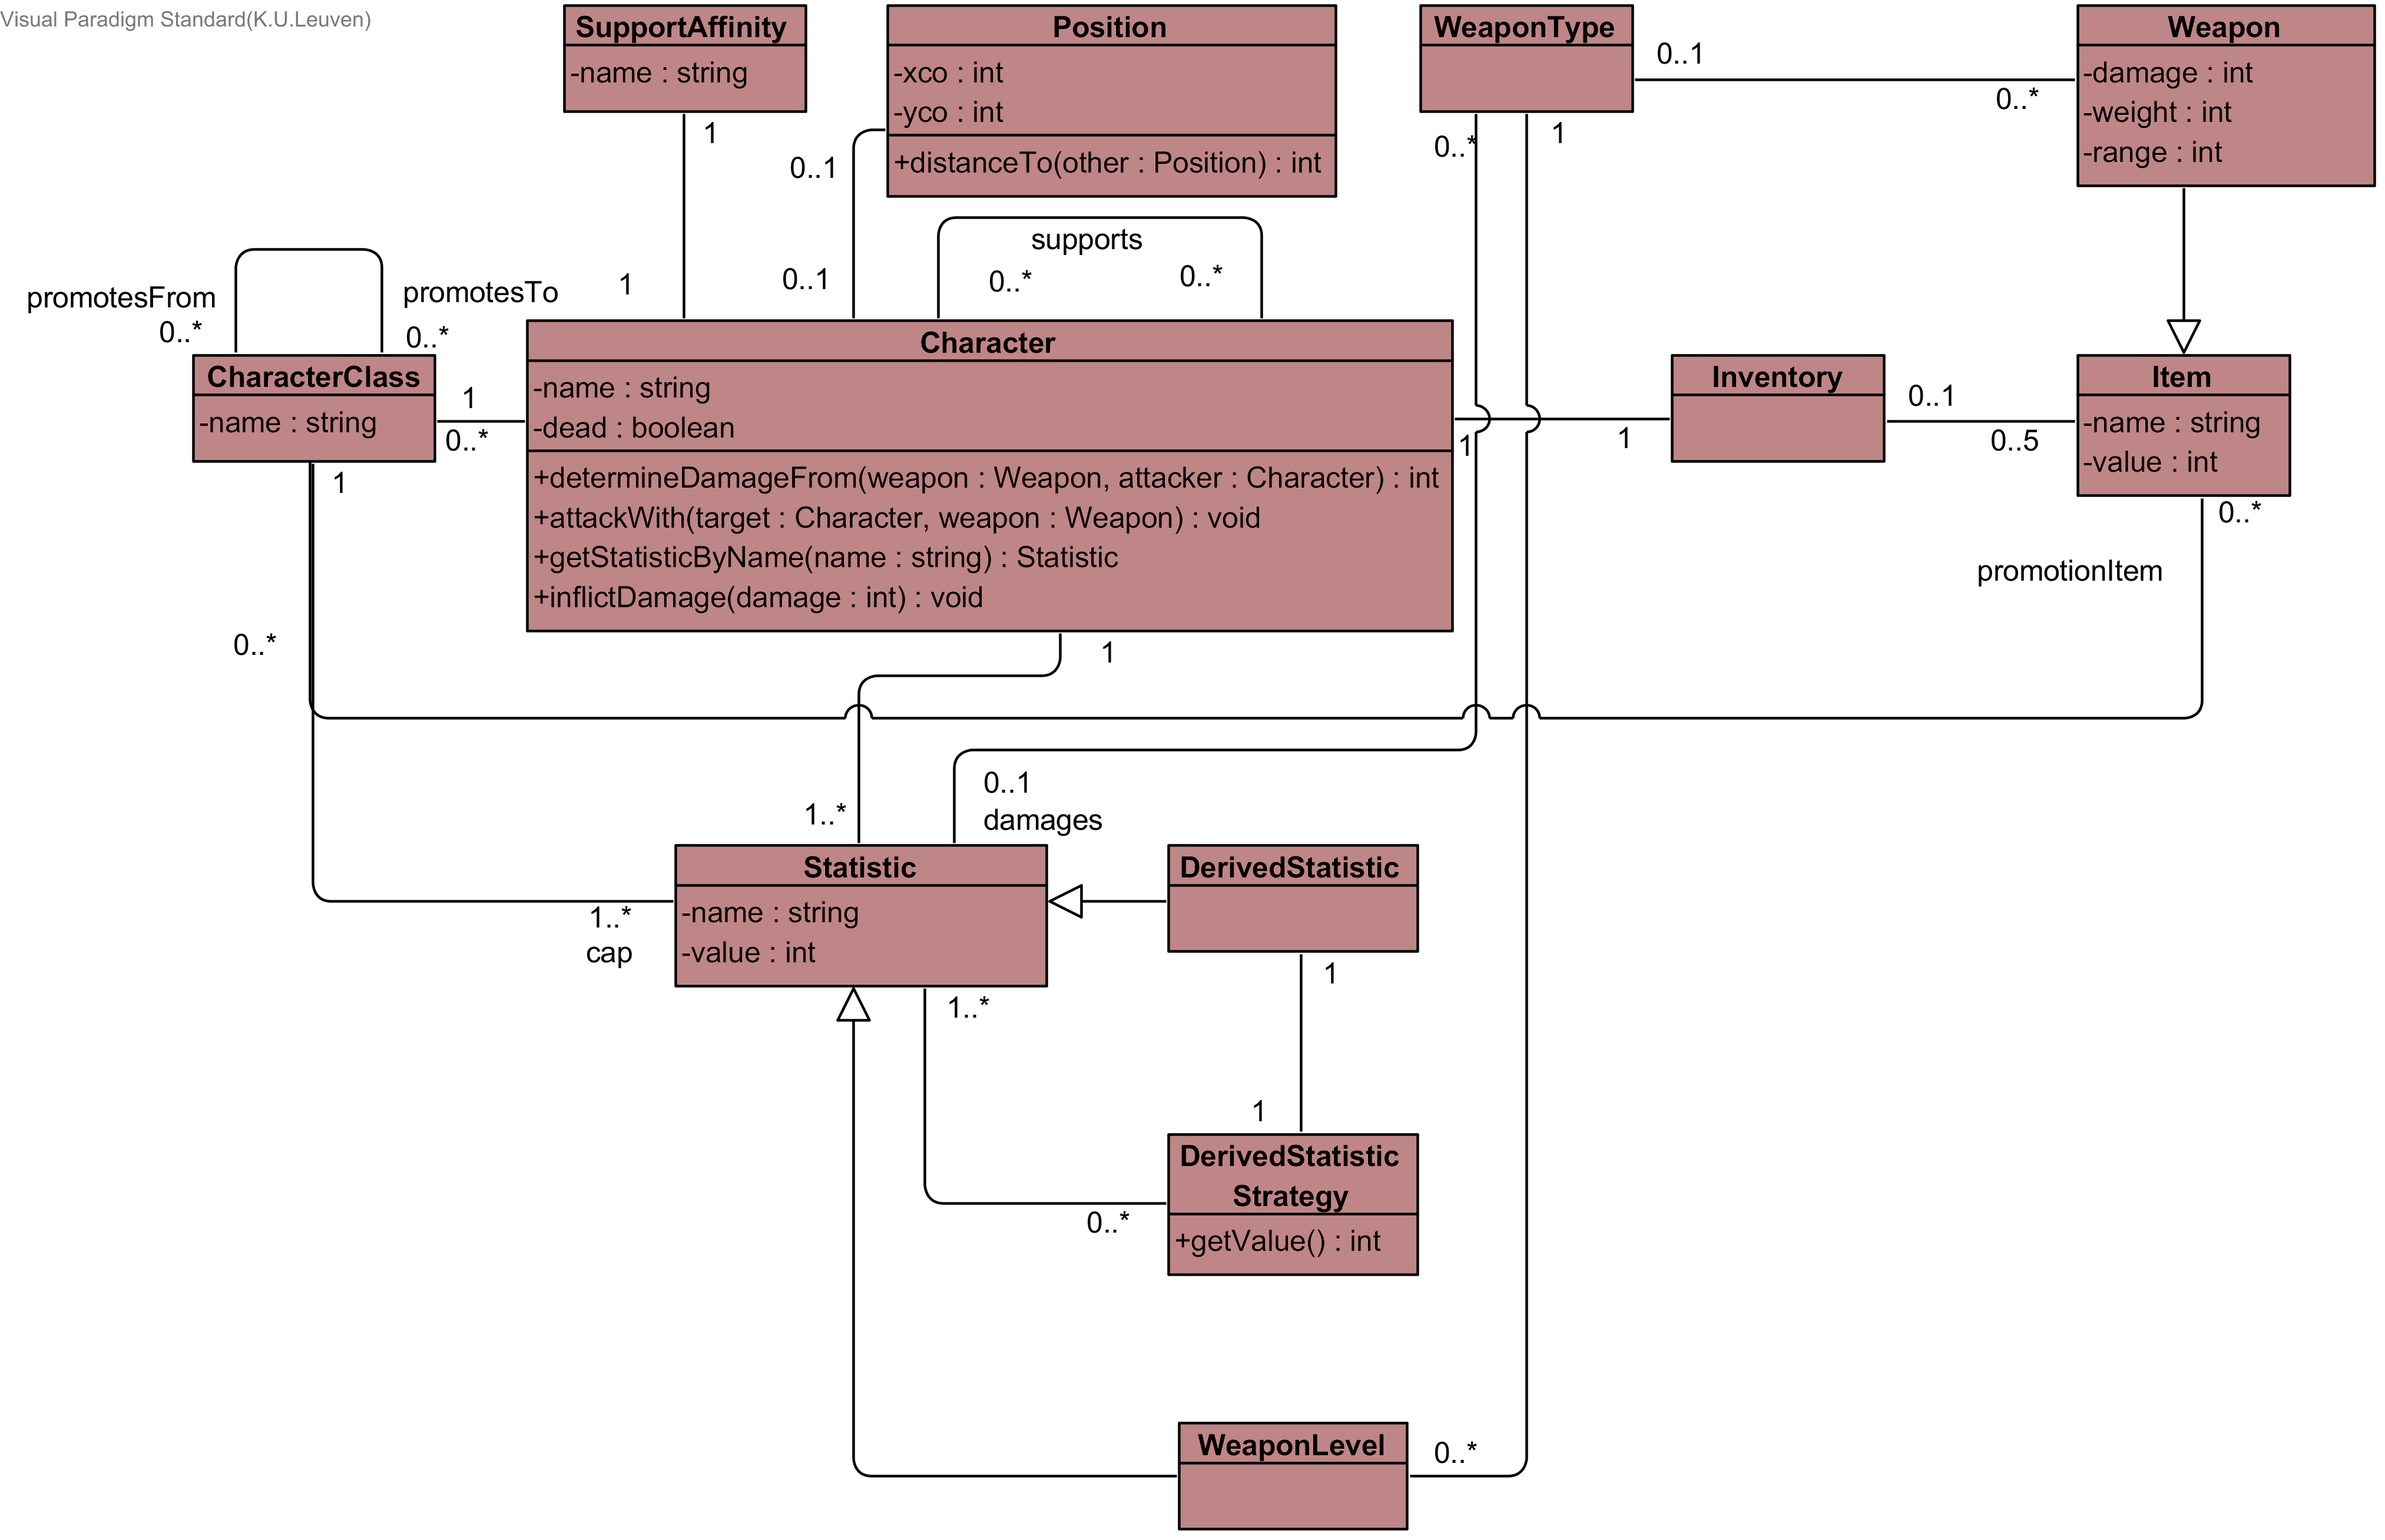
\includegraphics[width=0.95\textwidth]{chap-consistentie/diagram-voorbeeld.png}
	\caption{Leidend voorbeeld van een klassediagram}
\end{figure}

Meer bepaald willen we uitdrukken welke \textbf{klasses} er bestaan in het diagram waarvan een object een instantie kan zijn, welke \textbf{attributen} en \textbf{operaties} elke klasse bevat, welke \textbf{associaties} er bestaan tussen de verscheidene klasses en welke \textbf{klassehi\"erarchie\"en} er bestaan.

\subsection{Logisch type \textit{Object}}
Zoals gezegd staan in deze theori\"en objecten centraal, dus is het vanzelfsprekend om een logisch type \textit{Object} te voorzien. Dit logisch type bevat dus softwareobjecten.

\subsection{Logisch type \textit{ClassObject} en predicaat \textit{StaticClass$\backslash2$}}
Dit logisch type bevat exact de klasses die worden weergegeven in het diagram --- niet meer en niet minder. \textit{Character}, \textit{Inventory}, \textit{Item} enz. zijn dus \textit{ClassObject}s.
We drukken uit dat een \textit{Object} een instantie is van een bepaald \textit{ClassObject} door middel van het predicaat \textit{StaticClass$\backslash2$}. \textit{StaticClass(o1,Character)} zegt dus uit dat het object \textit{o1} een instantie is van klasse \textit{Character}.

\subsection{Voorstellen van attributen}
Voor elk attribuut voegen we een binair predicaat toe waarvan de naam beantwoordt aan het patroon: \textit{Klassenaamattribuutnaam}. Voor klasse \textit{Character} en attribuut \textit{name} resulteert dit dus in het predicaat \textit{Charactername$\backslash2$}. Het eerste argument van dit predicaat is een \textit{Object}. Het type van het tweede argument hangt af van wat er in het diagram staat: Als het een primitief type is zoals \textit{string} of \textit{int}, zal dat ook het type zijn van het tweede predicaat; in het andere geval is het type van het tweede argument ook \textit{Object}.
De signatuur van \textit{Charactername$\backslash2$} is daarom \textit{Charactername(Object, string)}.
Voor elk attribuut worden ook een aantal andere regels afgeleid:

\begin{itemize}
	\item Als het tweede argument van het attribuutpredicaat \textit{Object} is, wordt er een regel toegevoegd van de vorm:
	
	\begin{align*}
	\forall{o1}[Object]\forall{o2}[Object](Klassenaamattribuutnaam(o1,o2) \Rightarrow \\ StaticClass(classObj,o1) \land StaticClass(attrClassObj,o2))
	\end{align*}
	
	waarbij \textit{classObj} het logisch object van type \textit{ClassObject} dat het attribuut bevat en \textit{attrClassObj} het logisch object van type \textit{ClassObject} dat dient als mogelijke waarde van dit attribuut. Deze regel verzekert dat de attribuuthouder en de attribuutwaarde van de juiste klasse zijn. In dit diagram komt dit geval nergens voor en wordt deze regel dus niet toegepast.
	
	\item Als het tweede argument van het attribuutpredicaat van een primitief type is, wordt een regel toegevoegd van de vorm:
	
	\begin{align*}
	\forall{o}[Object]\forall{x}[primitiveType](Klassenaamattribuutnaam(o,x) \Rightarrow \\ StaticClass(classObj,o))
	\end{align*}
	
	waarbij primitiveType het type van de attribuutwaarde. De signatuur van het predicaat verzekert dat de attribuutwaarde van het juiste type is, dus moet dit niet explicit worden neergeschreven. Deze regel zorgt ervoor dat de volgende zin wordt toegevoegd aan de theorie:
	
	\begin{align*}
	\forall{o}[Object]\forall{x}[primitiveType](Charactername(o,x) \Rightarrow \\ StaticClass(Character,o))
	\end{align*}
	
	\item De multipliciteit van het attribuut wordt ook in rekening gebracht. Zij \textit{lowerBound} de ondergrens en \textit{upperBound} de bovengrens. Dan is de meest algemene vorm van deze regel als volgt:
	
	\begin{align*}
	\forall{o1}[Object](StaticClass(classObj,o1) \Rightarrow lowerBound \geq \\ \#\{o2: Klasseattribuutnaam(o1,o2)\} \geq upperBound
	\end{align*}
	
	waarbij \textit{lowerBound} wordt weggelaten als deze $0$ is en \textit{upperBound} wordt weggelaten als deze $*$ is. Indien beide van deze voorwaarden gelden, wordt er geen regel afgeleid betreffende de multipliciteit van het attribuut. Als $lowerBound = upperBound$, wordt deze regel in de plaats:
	
	\begin{align*}
	\forall{o1}[Object](StaticClass(classObj,o1) \Rightarrow \\ \exists_{=upperBound}{o2}(Klassenaamattribuutnaam(o1,o2))
	\end{align*}
	
	Voor \textit{Charactername$\backslash2$} wordt daarom afgeleid:
	
	\begin{align*}
	\forall{o}[Object](StaticClass(Character,o) \Rightarrow \exists_{=1}{x}(Charactername(o,x))
	\end{align*}
\end{itemize}

\subsection{Voorstellen van operaties}
Voor elke operatie voegen we een predicaat toe dat beantwoordt aan volgend patroon: \textit{Klassenaamoperatienaam$\backslash(m+2)$}, waarbij $m$ het aantal argumenten dat als invoer wordt meegegeven aan de operatie. De signatuur ziet eruit als \\ \textit{$Klasseoperatienaam(o,p_1,\ldots,p_m,r)$}, waarbij \textit{o} het object van logisch type \textit{Object} waarop de operatie wordt opgeroepen, \textit{$p_1$} \ldots \textit{$p_m$} de argumenten en \textit{r} het resultaat van de oproep van de operatie op het object \textit{o} met de gegeven argumenten. Indien er geen argumenten zijn, ziet de signatuur eruit als \textit{Klassenaamoperatienaam(o,r)}. Voor \textit{determineDamageWeaponFrom(Weapon)} van \textit{Character} wordt dit dus \textit{CharacterdetermineDamageFrom(Object,Object,int)}.

Voor elke operatie worden de volgende regels afgeleid:

\begin{itemize}
	\item Het object waarop de operatie wordt opgeroepen (zijnde \textit{o}), de parameters (zijnde \textit{$p_1 \ldots p_m$}) en het resultaat van de oproep (zijnde \text{r}) moeten allemaal van de juiste klasse zijn. Daarom wordt een regel toegevoegd van de vorm:
	
	\begin{align*}
	&\forall{o}[Object]\forall{p_1}[Object]\ldots\forall{p_m}[Object]\forall{r}[Object]
	\\
	&(Klassenaamoperatienaam(o,p_1,\ldots,p_m,r) \Rightarrow
	\\ 
	&StaticClass(classObj,o) \land StaticClass(p_{1}ClassObj,p_1) \land \ldots \land
	\\
	&StaticClass(p_{m}ClassObj,p_m) \land StaticClass(resultClassObj,r))
	\end{align*}
	
	Voor elke \textit{p} waarvoor geldt dat het van een primitief type is wordt de corresponderende \textit{StaticClass($p_l,p_{l}ClassObj$)} (met $1 \leq l \leq m$) weggelaten; hetzelfde geldt voor \textit{r}.
	De invulling voor \textit{CharacterdetermineDamageFrom(o,p1,r)} wordt dus:
	
	\begin{align*}
	\forall{o}[Object]\forall{p_1}[Object](CharacterdetermineDamageFrom(o,p_1,r) \Rightarrow \\
	StaticClass(Character,o) \land StaticClass(Weapon,p_1))
	\end{align*}
	
	\item Voor elke combinatie van Object waar de operatie wordt opgeroepen en invoerparameters moet gelden dat er exact \'e\'en resultaat is:
	
	\begin{align*}
	&\forall{o}[Object]\forall{p_1}[Object]\ldots\forall{p_m}[Object]
	\\
	&(StaticClass(classObj,o) \land StaticClass(p_{1}ClassObj,p_1) \land \ldots \land
	\\
	&StaticClass(p_m,p_{m}ClassObj) \Rightarrow
	\\
	&\exists!{r}[Object](Klassenaamoperatienaam(o,p_1,\ldots,p_m,r)))
	\end{align*}
	
	Opnieuw geldt dat voor primitieve types de bijhorende conjuncten weggelaten worden. De invulling voor \textit{CharacterdetermineDamageFrom(Object,Object,int)} wordt:
	
	\begin{align*}
	&\forall{o}[Object]\forall{p_1}[Object](StaticClass(Character,o) \land
	\\
	&StaticClass(Weapon,p_1) \Rightarrow \exists!{r}(CharacterdetermineDamageFrom(o,p1,r))
	\end{align*}
\end{itemize}

\subsection{Voorstellen van associaties}
Voor elke associatie voegen we een predicaat toe dat beantwoordt aan volgend patroon: \textit{$ClassOneand\ldots{}andClassM\backslash{m}$}, waarbij \textit{m} de ariteit van de associatie. Voor de associatie tussen \textit{Inventory} en \textit{Item} wordt dit dus \textit{InventoryandItem(Object,Object)}. We leiden regels van de volgende vormen af voor elke associatie:

\begin{itemize}
	\item De deelnemende Objects moeten allemaal van de juiste klasse zijn. Daarom wordt een regel toegevoegd van de vorm:
	
	\begin{align*}
	\forall{o_1}[Object]\ldots\forall{o_m}[Object](ClassOne\ldots{}andClassM(o_1,\ldots,o_m) \\ \Rightarrow StaticClass(o_{1}ClassObj,o_1) \land \ldots \land StaticClass(o_{m}ClassObj,o_m))
	\end{align*}
	
	Voor \textit{InventoryandItem(Object,Object)} wordt dit:
	
	\begin{align*}
	\forall{o_1}[Object]\forall{o_2}[Object](InventoryandItem(o1,o2) \Rightarrow \\ StaticClass(Inventory,o1) \land StaticClass(Item,o2))
	\end{align*}
	
	\item De multipliciteit voor elke rol moet worden uitgedrukt. Voor alle $o_l$ waarvoor $1 \leq l \leq m$ wordt een regel toegevoegd van de volgende vorm:\\
	Zij $lowerBound_l$ de ondergrens en $upperBound_l$ de bovengrens:
	\begin{align*}
	&\forall{c_1}[Object]\ldots\forall{c_m}[Object](StaticClass(c_{1}ClassObj,c_1) \land \ldots \land
	\\
	&StaticClass(c_{m}ClassObj,c_m) \Rightarrow lowerBound_l \leq
	\\
	&\#{o_l: ClassOneand\ldots{}ClassM(c_1,\ldots,o_1,\ldots,c_m)} \leq upperBound_l)
	\end{align*}
	
	waarbij de \textit{c} met index \textit{l} overgeslagen wordt. Indien de ondergrens gelijk is aan $0$ of de bovengrens gelijk is aan $*$ worden dezen weggelaten. Als beide voorwaarden gelden, wordt voor deze \textit{l} geen regel afgeleid. Indien $lowerBound_l = upperBound_l$ wordt in de plaats afgeleid:
	
	\begin{align*}
	&\forall{c_1}[Object]\ldots\forall{c_m}[Object](StaticClass(c_{1}ClassObj,c_1) \land \ldots \land
	\\
	&StaticClass(c_{m}ClassObj,c_m) \Rightarrow \\ &\exists_{=upperbound_l}o_l(ClassOneand\ldots{}andClassM(c_1,\ldots,o_l,\ldots,c_m)))
	\end{align*}
	
	Voor \textit{InventoryandItem$\backslash{}m$} worden de volgende regels afgeleid:
		\begin{align*}
		\forall{o_2}[Object](StaticClass(Item,o_2) \Rightarrow \\ \#{o_1: InventoryandItem(o_1,o_2)} \leq 1)
		\end{align*} 
		
		\begin{align*}
		\forall{o_1}[Object](StaticClass(Inventory,o_1) \Rightarrow \\ \#{o_2: InventoryandItem(o_1,o_2)} \leq 5)
		\end{align*}
\end{itemize}

\subsection{Voorstellen van klassehi\"erarchi\"een}
Stel dat voor een object \textit{o} van logisch type \textit{Object} gegeven is dat \textit{StaticClass(oClassObject,o)}. Ons doel is dat \textit{StaticClass(superClassObject,o)} geldt voor alle objecten van logisch type \textit{ClassObject} die volgens het diagram superklasses zijn van \textit{oClassObject} --- niet meer en niet minder. Daartoe introduceren we het predikaat \textit{IsDirectSupertypeOf(ClassObject,ClassObject)} dat ingevuld wordt door alle directe subklasseringen van het diagram en het predikaat \textit{IsSupertypeOf(ClassObject,ClassObject)}, hetgeen de transitieve sluiting is van \textit{IsDirectSupertypeOf}. Om zowel de invulling van \textit{IsDirectSupertypeOf$\backslash2$} te doen als de transitieve sluiting te berekenen maken we gebruik van \textbf{inductieve definities} voor twee redenen:

\begin{enumerate}
	\item In predikatenlogica is het onmogelijk om op een universeel geldige manier de transitieve sluiting uit te drukken.
	\item Als men in een inductieve definitie een lijst feiten opsomt, drukt men tegelijk ook uit dat exact die feiten waar zijn --- niet meer of niet minder.
\end{enumerate}

In \'e\'en definitie lijsten we dus de feiten die we kunnen aflezen van het diagram op:

\begin{align*}
\{
	IsDirectSupertypeOf(Statistic,Weaponlevel) \leftarrow \\
	IsDirectSupertypeOf(Statistic,DerivedStatistic) \leftarrow \\
	IsDirectSupertypeOf(Item,Weapon) \leftarrow \\
\}
\end{align*}

In een andere definitie drukken we de transitieve sluiting uit en gebruiken we die ook meteen om het gewenste resultaat voor \textit{StaticClass$\backslash2$} uit te komen:

\begin{align*}
\{
	&\forall{x}[ClassObject]\forall{y}[ClassObject](IsSupertypeOf(x,y) \leftarrow \\ &IsDirectSupertypeOf(x,y)) \\
	&\forall{x}[ClassObject]\forall{y}[ClassObject](IsSupertypeOf(y,x) \leftarrow \\
	&\exists{z}(IsSupertypeOf(y,z) \land IsSupertypeOf(z,x)))
	\\
	\\
	&\forall{x}[ClassObject]\forall{o}[Object](StaticClass(x,o) \leftarrow RuntimeClass(x,o)) \\
	&\forall{x}[ClassObject]\forall{y}[ClassObject]\forall{o}[Object](StaticClass(y,o) \leftarrow \\ &RuntimeClass(x,o) \land IsSupertypeOf(y,x))
\}
\end{align*}

waarbij \textit{RuntimeClass(ClassObject,Object)} een predikaat is dat uitdrukt wat de uniek dynamisch bepaalde klasse is van een \textit{Object} (de veronderstelling is dat in een geldige toestand van een programma in uitvoering ieder object exact \'e\'en \textit{runtime} klasse heeft).
\\
In hoofdstuk \ref{sec:rol-idp} wordt de logische theorie die automatisch gegenereerd werd volgens de regels opgelijst in dit hoofdstuk weergegeven en wordt ook uitgelegd hoe die theorie wordt gebruikt om de consistentie van het diagram te controleren.
\chapter{Controleren op kwaliteitsgebreken}\label{sec:kwaliteitsgebrek}
Waar in hoofdstuk \ref{sec:consistentie} \textit{Object}s centraal stonden, doen we daar hier afstand van: we abstraheren \textit{Object}s weg en concentreren ons in de plaats op \textit{ClassObject}s. We gebruiken het diagram in figuur \ref{fig:diagram-voorbeeld} weer als begeleidend voorbeeld. In de volgende subsecties overlopen we hoe we de theorie die we gebruiken voor dit probleem opbouwen.

\subsection{Gebruikte logische types en predikaten}
We bewaren het logisch type \textit{ClassObject} en het predikaat \textit{IsSupertypeOf(ClassObject,\\ClassObject)} exact zoals ze zijn in hoofdstuk \ref{sec:consistentie} (en berekenen de transitieve sluiting horende bij \textit{IsSupertypeOf$\backslash2$} op dezelfde manier) en gebruiken daar bijkomend volgende predikaten:

\begin{itemize}
	\item \textbf{\textit{BiAssoc(ClassObject,ClassObject)}}: drukt uit dat er een binaire associatie bestaat tussen de twee klasses.
	\item \textbf{\textit{BiAssocLow(ClassObject,ClassObject,ClassObject,nat)}}: voor \textit{BiAssocLow(x,y,x,n1)} geldt dat voor de binaire associatie tussen klasse \textit{x} en klasse \textit{y} de ondergrens voor de multipliciteit aan de \textit{x}-kant gelijk is aan \textit{n1}; een gelijkaardige interpretatie geldt voor \textit{BiAssocLow(x,y,y,n2)}.
	\item \textbf{\textit{BiAssocHigh(ClassObject,ClassObject,ClassObject,nat)}}: gelijkaardig aan \textit{BiAssocLow$\backslash4$}, maar dan voor de bovengrens van de multipliciteit.
\end{itemize}

Deze predikaten worden ingevuld met een lijst van feiten die af te lezen zijn van het diagram. In hoofdstuk \ref{sec:rol-idp} wordt de logische theorie die het resultaat is van dit proces weergegeven.

\subsection{Kwaliteitsgebreken detecteren}
Er zijn drie kwaliteitsgebreken waarnaar wordt gezocht in de resulterende theorie:

\begin{itemize}
	\item \textbf{Many-to-many associaties}: Dit zijn associaties waar dat de bovengrens van de multipliciteiten aan beide kanten gelijk is aan $*$. Het voorkomen van een many-to-many associatie is doorgaans een teken dat er een klasse ontbreekt in het ontwerp. Het is dus van groot belang dat dit wordt opgespoord en opgelost.
	
	\item \textbf{Losstaande klasse}: Concreet is een losstaande klasse een klasse die geen associatie heeft met een andere klasse in het ontwerp. Zulk een klasse is nutteloos en moet ofwel verbonden worden met een andere klasse of verwijderd worden.
	
	\item \textbf{Overbodige associaties in een klassehi\"erarchie}: Beschouw figuur \ref{fig:hierarchie}. Daar is te zien dat de grenzen van de multipliciteiten in de associatie \textit{Alice}---\textit{Charlie} strengere voorwaarden opleggen dan die van de associatie \textit{Bob}---\textit{David}, en dat daarom de associatie \textit{Bob}---\textit{David} overbodig is. Om de verstaanbaarheid van het diagram te verbeteren, wordt die associatie best verwijderd.
\end{itemize}

We defini\"eren deze respectievelijke gebreken in de logische theorie door middel van de volgende logische zinnen:

\begin{align*}
	\forall{x}[ClassObject]\forall{y}[ClassObject](ManyToMany(x,y) \Leftrightarrow BiAssoc(x,y) \land \\ \lnot\exists{z}[nat](BiAssocHigh(x,y,x,z)) \land \lnot\exists{z}[nat](BiAssocHigh(x,y,y,z)))
\end{align*}

\begin{align*}
	\forall{x}[ClassObject](LooseClass(x) \Leftrightarrow \lnot(\exists{y}[ClassObject](BiAssoc(x,y)) \\ \lor \exists{s}[ClassObject]\exists{y}[ClassObject](IsSupertypeOf(s,y) \land BiAssoc(s,x)))
\end{align*}

\todo{oplossing vinden voor de derde: gewoon verwijzen naar IDP-bestand?}

\begin{figure}
	\label{fig:hierarchie}
	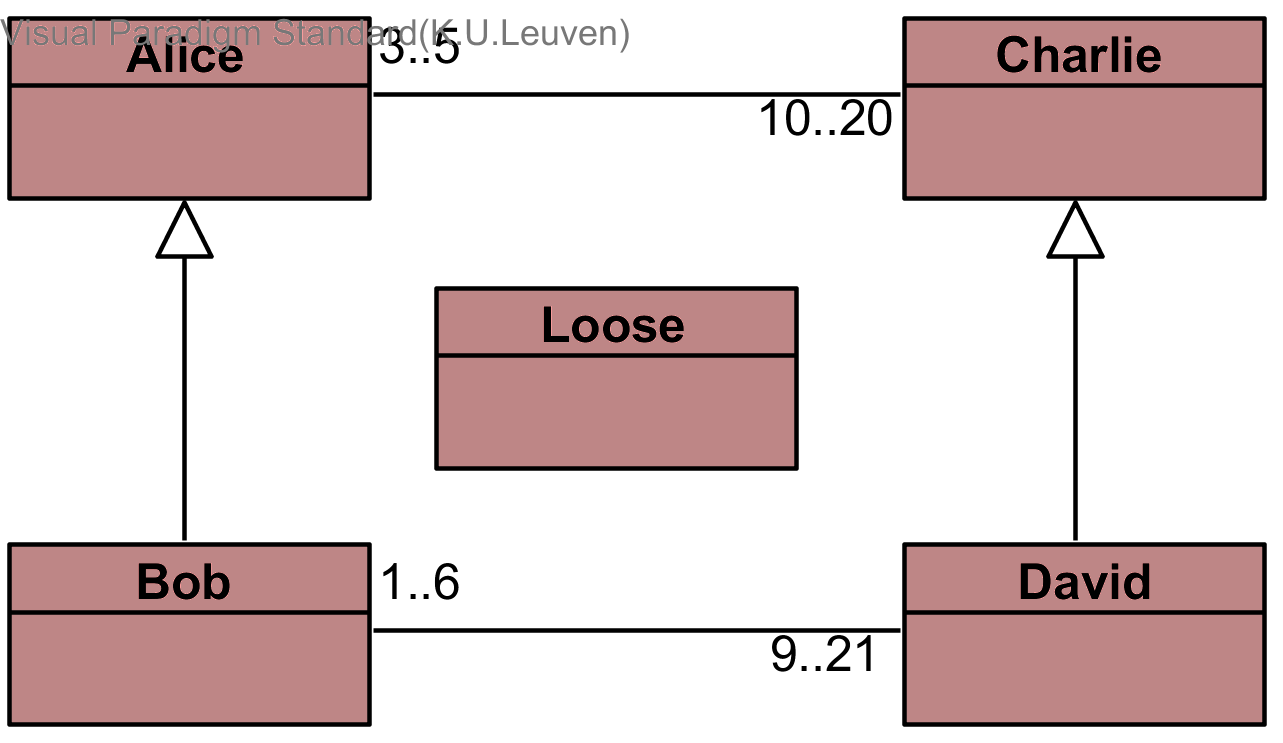
\includegraphics{chap-kwaliteitsgebrek/hierarchy.png}
	\caption{Voorbeeld van meer permissieve multipliciteiten in een klassehi\"erarchie en van een losstaande klasse (zijnde \textit{Loose})}
\end{figure}

Deze regels worden meteen toegevoegd aan de theorie die wordt gegenereerd zoals uitgelijnd eerder in dit hoofdstuk. In hoofdstuk \ref{sec:rol-idp} wordt uitgelegd hoe deze theorie wordt gebruik om kwaliteitsgebreken te vinden.
\chapter{Het kennisbanksysteem IDP}\label{sec:rol-idp}
\section{Korte inleiding in IDP}
IDP is een kennisbanksysteem\cite{DeCatBroes2014PLaa}. Deze kennisbanken zijn opgesteld in FO($\cdot$), een uitbreiding van predicatenlogica. De basisblokken van een specificatie in IDP zijn als volgt:

\begin{itemize}
	\item \textbf{Vocabularium}: Hier specificeert de ontwerper de logische types die bestaan in het beschouwd domein en de predicaten en functies over die logische types.
	\item \textbf{Theorie}: Hier schrijft de ontwerper zinnen in FO($\cdot$) die bepalen welke structuren over het beschouwde vocabularium modellen zijn. Indien de ontwerper een inconsistente theorie ontwerpt, zullen er geen modellen zijn.
	\item \textbf{Structuur}: De ontwerper vult hier de logische types gedefinieerd in het vocabularium in. \textit{Constructed types} hebben geen invulling nodig aangezien ze al volledig worden gespecificeerd in het vocabularium. De ontwerper kan ook voor \'e\'en of meerdere predicaten aangeven welke tupels wel of geen lid zijn. Hij kan ook voor \'e\'en of meerdere functies specificeren welke elementen uit het domein afgebeeld worden op welk element uit het codomein.
\end{itemize}

De ontwerper kan meerdere vocabularia, theorie\"en en structuren neerschrijven. Elke theorie en structuur kan wel maar de symbolen van \'e\'en vocabularium gebruiken.

IDP gebruikt zijn eigen symbolen voor universele kwantoren, existenti\"ele kwantoren en logische connectieven. \cite{DeCatBroes2014PLaa} bevat een uitgebreidere inleiding tot IDP.

\section{Gebruik van modeluitbreiding}
Gegeven een structuur over een bepaald vocabularium kan de gebruiker de opdracht geven aan IDP om een uitbreiding te vinden van deze structuur die ervoor zorgt de structuur een model is van een gegeven theorie. Dit is een vorm van inferentie die men \textbf{modeluitbreiding} noemt. Het kan echter het geval zijn dat IDP antwoordt dat zulk een uitbreiding niet bestaat of dat de uitvoering nooit eindigt.


\subsection{Controleren van consistentie}
In bijlage \ref{app:consistentie} staat de logische theorie die werd gegenereerd volgens de regels uitgelijnd in hoofdstuk \ref{sec:consistentie}. Als men dit geeft als invoer aan IDP, is het besluit dat er een model bestaat voor de theorie en dat het diagram inderdaad consistent is.

\subsection{Detecteren van kwaliteitsgebreken}
In bijlage \ref{app:kwaliteitsgebrek} staat de logische theorie die werd gegenereerd uit een combinatie van de diagrammen uit figuren \ref{fig:diagram-voorbeeld} en \ref{fig:hierarchie} volgens de regels uitgelijnd in hoofdstuk \ref{sec:kwaliteitsgebrek}. IDP vindt alle many-to-many associaties, besluit dat \textit{Loose} een losstaande klasse is en dat de associatie \textit{Bob}---\textit{David} overbodig is door de samenloop van de klassehi\"erarchie en de opgelegde multipliciteiten.
\chapter{Simuleren van gedrag op basis van een sequentiediagram}\label{sec:gedrag}
Een ander populair type van UML-diagram is het sequentiediagram. Waar klassediagrammen de informatie bevat in klasses en de verbanden tussen klasses benoemen, beschrijven sequentiediagrammen het gedrag van methodes gedefinieerd voor deze klasses. In deze diagrammen communiceren instanties van klasses via berichten. Doorgaans zijn deze berichten een oproep van een methode, of een toekenning aan een variabele intern aan het diagram of een instantiatie van een nieuwe instantie. De berichten zijn genummerd volgens een bepaalde volgorde en samen modelleren ze het gedrag van een stuk van de software.

\parbreak

Figuur \ref{fig:seq-diagram-game} geeft een voorbeeld van een sequentiediagram gebaseerd op het klassediagram voorgesteld in figuur \ref{fig:diagram-voorbeeld}.

Een instantie wordt voorgesteld door een kader met daarin tekst volgens het patroon \textit{instantienaam : klassenaam}. Dit wil zeggen dat bijvoorbeeld \textit{attacker} een instantie is van de klasse \textit{Character}. Vanuit elk kader vertrekt ook een streepjeslijn: De \textbf{levenslijn}. Deze levenslijn kan ingevuld worden door gekleurde balken, welke de duur van een oproep van een methode aan een instantie voorstellen.
Verder zijn er ook kaders die berichten omsluiten. Deze kaders duiden \textbf{gecombineerde fragmenten} aan, en in deze tekst beschouwen we twee soorten:

\begin{enumerate}
	\item Het \textbf{altfragment}: Deze soort duidt een \textit{if-else}-constructie aan. Het bestaat uit twee delen, namelijk het \textit{if}-deel en het \textit{else}-deel, en er staat aangeduid onder welke voorwaarden welk deel wordt uitgevoerd. Figuur \ref{fig:seq-diagram-game} bevat een voorbeeld van een altfragment.
	\item Het \textbf{lusfragment}: Deze soort duidt een lusconstructie aan. Er staat aangeduid onder welke voorwaarden er een iteratie wordt uitgevoerd. Deze voorwaarde wordt gecontroleerd zowel v\'o\'or de eerste keer dat er mogelijks een iteratie wordt uitgevoerd als elke keer dat een iteratie ten einde komt. Indien de voorwaarde niet geldt, wordt de lus overgeslagen. Figuur \ref{fig:seq-diagram-frag-ex} bevat een voorbeeld van een diagram met lusfragmenten.
\end{enumerate}

In dit hoofdstuk beschouwen we hoe we het vocabularium en de logische theorie die we hebben opgebouwd eerder in de tekst kunnen uitbreiden om het gedrag voorgesteld in een sequentiediagram te modelleren.

\begin{landscape}
	\thispagestyle{empty}
\begin{figure}
	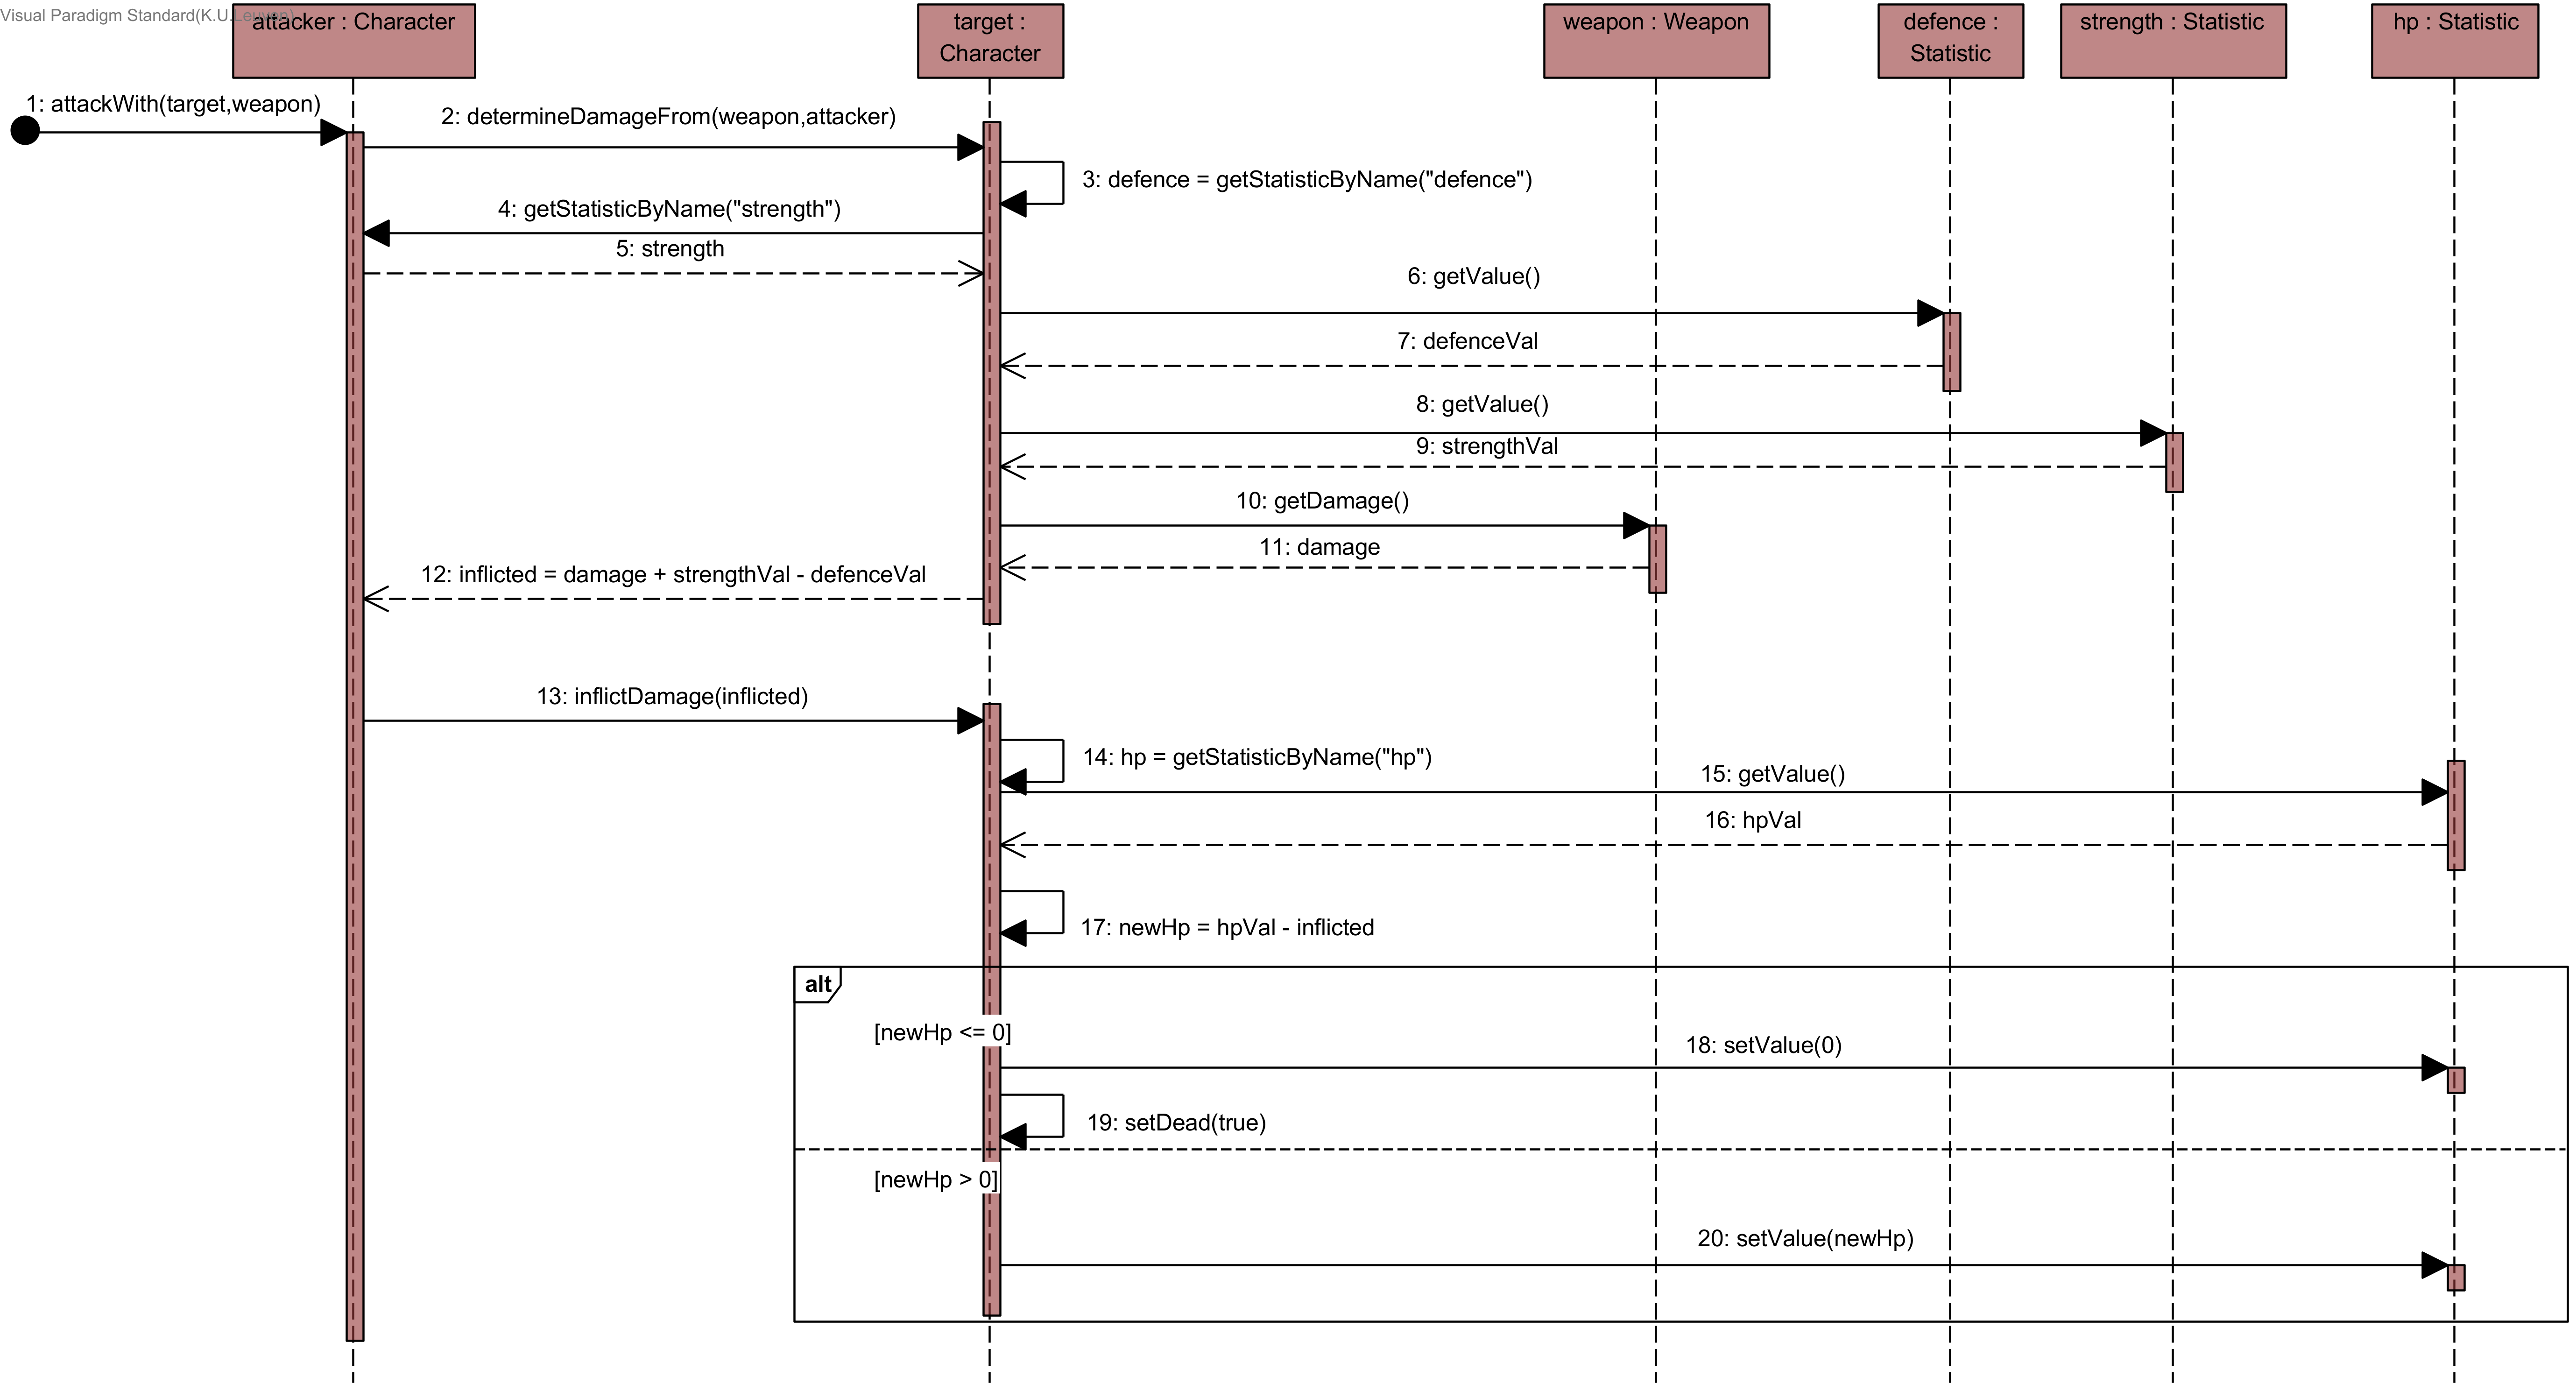
\includegraphics[width=1.5\textwidth]{chap-gedrag/seq-diagram-game.png}
	\caption{Sequentiediagram gebaseerd op het klassediagram van figuur \ref{fig:diagram-voorbeeld}}
	\label{fig:seq-diagram-game}
\end{figure}
\end{landscape}

\section{De keuze voor lineaire tijdscalculus}
UML-diagrammen schrijven mogelijke toestanden van softwaresystemen en acties op deze voor. Die systemen kunnen van toestand veranderen tussen tijdstappen. Sequentiediagrammen zijn een manier om te beschrijven hoe zulke veranderingen teweeggebracht kunnen worden. Tijdens de uitvoering van een sequentiediagram mag het systeem enkel veranderen zoals beschreven door de huidige actie. Daarom hebben we een mechanisme nodig binnen FO($\cdot$) dat dynamische systemen en bewerkingen erop kan beschrijven. Tegelijk moet dat mechanisme garanderen dat eigenschappen van het systeem die niet worden be\"invloed door de huidige beschouwde actie van het sequentiediagram niet veranderen. Lineaire tijdscalculus\cite{BogaertsBart2014Sdsu}, oftewel LTC, voldoet aan deze voorwaarden. Daarom zullen we om sequentiediagrammen uitvoerbaar te maken binnen FO($\cdot$) het generatieproces voor het vocabularium en de theorie die we bekomen hebben in hoofdstuk \ref{sec:consistentie} uitbreiden volgens de principes van LTC. Dit betekent dat we de predicaten voor operaties die voorheen gegenereerd werden in hoofdstuk \ref{sec:consistentie} achterwege laten.

In de volgende secties werken we deze uitbreiding uit voor het sequentiediagram in figuur \ref{fig:seq-diagram-game}.

\section{Uitbreiding van het vocabularium}
In LTC is tijd een centraal concept, dus daarom introduceren we allereerst een logisch type $Time \subset \mathbb{N}$. Verder defini\"eren we een parti\"ele functie \textit{Next(Time)} dat voor alle tijdpunten het volgende tijdpunt geeft behalve voor het laatst mogelijke tijdpunt. We defini\"eren ook een constante \textit{Start}, wat het eerst mogelijke tijdpunt aanduidt.

Voor elk tijdpunt is het mogelijk dat er een bepaalde instructie van het sequentiediagram wordt uitgevoerd. We duiden deze instructie aan met zijn volgnummer.
Deze volgnummers gebruiken we als instructieteller, en daarvoor defini\"eren we een logisch type $SDPoint \subset \mathbb{N}$.

Om te garanderen dat de instructievolgorde opgelegd door het sequentiediagram gevolgd wordt, maken we deze instructieteller inertieel en introduceren we deze symbolen:

\begin{itemize}
	\item Het toestandspredicaat: \textit{SDPointAt(Time, SDPoint)}
	\item Het begintoestandspredicaat: \textit{I\_SDPointAt(SDPoint)}
	\item Het causatiepredicaat: \textit{C\_SDPointAt(Time, SDPoint)}
\end{itemize}

We moeten ook de instanties waarop gehandeld wordt in het sequentiediagram kunnen benoemen. Om te garanderen dat de instanties die vernoemd worden altijd verwijzen naar hetzelfde object tenzij een instructie een toekenning doet aan de overeenkomstige variabele, maken we ook de instanties inertieel. Voor \textit{attacker} verkrijgen we dan bijvoorbeeld:

\begin{itemize}
	\item \textit{AttackerT(Time, Character)}
	\item \textit{I\_AttackerT(Character)}
	\item \textit{C\_AttackerT(Time, Character)}
\end{itemize}

Het is ook mogelijk dat in een instructie een variabele intern aan het sequentiediagram wordt gedefinieerd. Zo is er instructie 7 waar een \textit{return}-instructie \textit{defenceVal} definieert en ook instructie 12 die de waarde van \textit{inflicted} definieert als een som van andere variabelen. Deze variabelen willen we ook kunnen benoemen en maken we inertieel. Voor alle zulke variabelen defini\"eren we ook predicaten zoals hierboven voor \textit{attacker}.

We passen ook de predicaten die overeenkomen met klasseattributen aan. Het kan immers zijn dat de waarde van een attribuut wordt aangepast, zoals in instructie 18 die de waarde van \textit{value} van object \textit{hp} van klasse \textit{Statistic} verandert naar 0. Klasseattributen maken we ook inertieel. Voor \textit{value} in \textit{Statistic} krijgen we dan:

\begin{itemize}
	\item \textit{Statisticvalue(Time, Statistic, LimitedInt)}
	\item \textit{I\_Statisticvalue(Statistic, LimitedInt)}
	\item \textit{C\_Statisticvalue(Time, Statistic, LimitedInt)}
	\item En het oncausatiepredicaat: \textit{Cn\_Statisticvalue(Time, Statistic, LimitedInt)}
\end{itemize}

Hier voegen we een oncausatiepredicaat toe omdat het mogelijk is dat een attribuut meer dan \'e\'en waarde heeft op een bepaald tijdstip als de bovengrens voor de multipliciteit groter is dan \'e\'en. Met dit predicaat geven we aan dat bepaalde waardes die voor een bepaalde tijdstap gelden ongedaan moeten worden gemaakt in de volgende tijdstap.

\section{Uitbreiden van de theorie}
Voor elke inerti\"ele eigenschap van het systeem moeten er twee dingen gebeuren: Toestandszinnen opstellen en voorwaardes voor causatiezinnen en oncausatiezinnen specificeren. Het resultaat is een inductieve definitie die de inerti\"ele predicaten definieert en een inductieve definitie die de causatiepredicaten en oncausatiepredicaten definieert.

\subsection{Toestandszinnen opstellen}
Toestandszinnen worden geschreven in termen van begintoestandspredicaten, causatiepredicaten en oncausatiepredicaten. Ze garanderen dat inerti\"ele eigenschappen enkel veranderen wanneer het ook echt de bedoeling is dat ze veranderen.

Als eerste kijken we naar toestandszinnen voor \textit{SDPointAt/2}. \textit{I\_SDPointAt/1} geeft aan welke de eerste instructie is die we willen uitvoeren, en daarom schrijven we een definitie die deze overeenkomst uitdrukt:

\begin{align}
	\forall{s}[SDPoint](SDPointAt(Start, s) \leftarrow I\_SDPointAt(s)).
\end{align}


De volgende definities gebruiken het causatiepredicaat:

\begin{align}
	\forall{t}[Time]\forall{s}[SDPoint](SDPointAt(Next(t), s) \leftarrow C\_SDPointAt(Next(t), s)). \label{eq:sdcauses}
\end{align}
\begin{align}
	\forall{t}[Time]\forall{s}[SDPoint](SDPointAt(Next(t), s) \leftarrow SDPointAt(t, s) \nonumber \\ \land{} \space \lnot{}(\exists{s1}[SDPoint](C\_SDPointAt(Next(t), s1)))). \label{eq:sduncauses}
\end{align}

Zin \ref{eq:sduncauses} zorgt ervoor dat de huidige waarde van \textit{SDPointAt} wordt behouden tenzij er een oorzaak is voor verandering.

We schrijven gelijkaardige definities voor de predicaten die overeenkomen met instanties die vernoemd worden in het sequentiediagram (zoals \textit{attacker}).

\parbreak

Voor klasseattributen verloopt dit ook gelijkaardig, maar we wijken af van het formaat van zin \ref{eq:sduncauses} door als volgt het oncausatiepredicaat te gebruiken:

\begin{align*}
	\forall{t}[Time]\forall{s}[Statistic]\forall{i}[LimitedInt](Statisticvalue(Next(t), s, i) \\ \leftarrow Statisticvalue(t, s, i) \land \lnot Cn\_Statisticvalue(Next(t), s, i)).
\end{align*}

\subsubsection{Voorwaardes voor causatie en oncausatie}
We kijken eerst naar klasseattributen. Een aantal ervan worden niet aangepast, wat we bijvoorbeeld neerschrijven voor \textit{range} in \textit{Weapon} als volgt:

\begin{align*}
	\forall{t}[Time]\forall{w}[Weapon]\forall{i}[LimitedInt](C\_Weaponrange(t, w, i) \leftarrow false).
\end{align*}
\begin{align*}
	\forall{t}[Time]\forall{w}[Weapon]\forall{i}[LimitedInt](Cn\_Weaponrange(t, w, i) \leftarrow false).
\end{align*}

Voor de klasseattributen die wel worden aangepast, kijken we naar de instructies die zulke aanpassingen doorvoeren. Voor \textit{value} in \textit{Statistic} zijn dit instructie 18 en 20. We kijken eerst naar de causatiezin en oncausatiezin die volgen uit instructie 18:

\begin{align*}
	\forall{t}[Time]\forall{s}[Statistic](C\_Statisticvalue(t, s, 0) \leftarrow SDPointAt(t, 18) \land HpT(t, s).
\end{align*}
\begin{align*}
	\forall{t}[Time]\forall{s}[Statistic]\forall{i}[LimitedInt](Cn\_Statisticvalue(Next(t), s, i) \\ \leftarrow SDPointAt(Next(t), 18) \land HpT(t, s) \land Statisticvalue(t, s, i) \land \lnot{}(i = 0).
\end{align*}

Aangezien in instructie 18 de instantie \textit{hp} wordt aangesproken, gebruiken we \textit{HpT/2} om te verzekeren dat de waarde van het juiste logisch object wordt veranderd. \textit{value} kan ook maar \'e\'en waarde tegelijk hebben, en daarom schrijven we een oncausatiezin om te verzekeren dat de vorige waarde wordt gewist.

Kijken we nu naar de definities die voortvloeien uit instructie 20:

\begin{align*}
	&\forall{t}[Time]\forall{s}[Statistic]\forall{i}[LimitedInt](C\_Statisticvalue(t, s, i) \\ &\leftarrow SDPointAt(t, 20) \land HpT(t, s) \land NewHpT(t, i)).
\end{align*}
\begin{align*}
&\forall{t}[Time]\forall{s}[Statistic]\forall{i}[LimitedInt](Cn\_Statisticvalue(Next(t), s, i) \\ &\leftarrow SDPointAt(Next(t), 20) \land HpT(t, s) \land Statisticvalue(t, s, i) \land \\ &\lnot{}NewHpT(Next(t), i)).
\end{align*}

Het verschil hier is dat we \textit{NewHpT} erbij betrekken omdat we de waarde van \textit{hp} veranderen naar de waarde van \textit{newHp} in plaats van het te veranderen naar 0.

\parbreak

Het volgende waar we naar kijken zijn de causatiezinnen voor \textit{SDPointAt/2}. Wat we hier willen uitdrukken is dat normaal gezien tussen instructies de instructieteller telkens met \'e\'en wordt verhoogd, tenzij een grens van een \textit{if-else}-constructie of een lus is bereikt. In dat geval kan het zijn dat de instructieteller verspringt afhankelijk van de voorwaarde die vernoemd wordt voor zulke constructies.

Voor deze sequentiediagram krijgen we:

\begin{align}
	&\forall{t}[Time]\forall{s}[SDPoint](C\_SDPointAt(Next(t), (s+1) \leftarrow SDPointAt(t, s) \nonumber \\ &\land \lnot{}((s = 17) \lor (s = 19))). \label{eq:sdprog} \\
	&\forall{t}[Time](C\_SDPointAt(Next(t), 18) \leftarrow SDPointAt(t, 17) \land \nonumber \\ &(\exists{i}[LimitedInt](NewHpT(t, i) \land i <= 0))). \label{eq:sdif} \\
	&\forall{t}[Time](C\_SDPointAt(Next(t), 20) \leftarrow SDPointAt(t, 17 ) \land \nonumber \\ &(\exists{i}[LimitedInt](NewHpT(t, i) \land i > 0))). \label{eq:sdthen} \\
	&\forall{t}[Time](C\_SDPointAt(Next(t), 21) \leftarrow SDPointAt(t, 19) \lor SDPointAt(t, 20)). \label{eq:sdexit}
\end{align}

Zin \ref{eq:sdprog} verzekert het juiste gedrag van de instructieteller, namelijk dat hij doorgaans met \'e\'en wordt verhoogd tussen tijdstappen. De uitzonderingen worden hier ook opgelijst; in dit geval verspringt de teller wanneer men het begin van de \textit{if-else}-constructie tegenkomt en wanneer het einde van het \textit{if}-deel is bereikt. Zinnen \ref{eq:sdif} en \ref{eq:sdthen} controleren de voorwaarde voor de uitvoering van het \textit{if}- en \textit{else}-deel en selecteren wat correct is. Zin \ref{eq:sdexit} zegt dat zowel het \textit{if}-deel als het \textit{else}-deel uitkomen op de instructie die direct volgt op de \textit{if-else}-constructie.

Voor dit diagram is het eenvoudig om deze zinnen op te stellen aangezien er geen geneste gecombineerde fragmenten aanwezig zijn. We beschrijven de algemene methode om het uitvoeringspad doorheen gecombineerde fragmenten te bepalen in sectie \ref{sec:combined-fragment}.

\parbreak

Als laatste zijn er de causatiezinnen voor de verscheidene variabelen die worden aangemaakt en aangesproken in het sequentiediagram. Een aantal van deze variabelen veranderen niet doorheen de uitvoering van het sequentiediagram en er wordt verondersteld dat deze al bekend zijn v\'o\'or de uitvoering begint. Deze variabelen zijn diegenen die betrokken zijn bij de eerste instructie: \textit{attacker}, de instantie die de eerste oproep ontvangt, en \textit{target} en \textit{weapon}, die als parameter worden opgegeven.

Voor de andere variabelen wordt er een causatiezin toegevoegd voor elke instructie die een waarde toekent aan die variabele. Als voorbeeld bekijken we instructie 3:

\begin{align*}
	&\forall{t}[Time]\forall{d}[Statistic](C\_DefenceT(t, d) \leftarrow SDPointAt(t, 3) \land \\ &\exists{c}[Character](TargetT(t, c) \land CharacterandStatistic(c, d) \\ &\land Statisticname(t, d, "defence"))).
\end{align*}


De zin drukt uit dat de getter wordt opgeroepen op \textit{target} en dat er wordt gevraagd naar een instantie van \textit{Statistic} dat in verband staat met \textit{target} en als naam ``defence'' heeft. Die instantie wordt dan als waarde toegekend aan de variabele \textit{defence}.

Zie bijlage \ref{app:seq-diagram-game} voor het volledig model voor het gedrag van het sequentiediagram in figuur \ref{fig:seq-diagram-game}.


\section{Het uitvoeren van gecombineerde fragmenten}\label{sec:combined-fragment}
Het opstellen van causatiezinnen voor \textit{SDPointAt/2} ten gevolge van gecombineerde fragmenten is niet vanzelfsprekend. In deze sectie beschrijven we onze methode om dit te bewerkstelligen.
Bij de vertaling van sequentiediagrammen houden we in de interne voorstelling binnen onze vertaler van een gecombineerd fragment volgende zaken bij:

\begin{itemize}
	\item Alle gecombineerde fragmenten die kinderen zijn van het fragment.
	\item Het fragment dat de ouder is van het fragment in kwestie, als die bestaat.
	\item Alle berichten die rechtstreeks deel zijn van het fragment. Een bericht is rechtstreeks deel van een fragment als het bericht een deel is van het fragment, maar geen rechtstreeks deel is van een kind of afstammeling van het fragment.
	\item De voorwaarde waaraan voldaan moet zijn om het fragment uit te voeren. 
\end{itemize}

Voor alt-fragmenten maken we het onderscheid tussen kinderen en berichten van het \textit{if}-gedeelte enerzijds en tussen kinderen en berichten van het \textit{else}-gedeelte anderzijds. Ook geldt dat er een voorwaarde is voor de uitvoering van het \textit{if}-gedeelte en voor de uitvoering van het \textit{else}-gedeelte.

In de methode om in de uitvoertheorie het uitvoeringspad doorheen gecombineerde fragmenten correct te vertalen gebruiken we drie procedures: E\'en die bepaalt naar welke berichten wordt gesprongen onder welke voorwaarde bij het binnengaan van een fragment, \'e\'en die bepaalt naar welke berichten wordt gesprongen onder welke voorwaarde bij het buitengaan van een fragment en \'e\'en die de heruitvoering van een lus verzorgt indien de voorwaarde voor de lus nog geldt. We bespreken deze procedures afzonderlijk.

\subsection{Transitie naar een fragment}\label{sec:transition-to}

Het resultaat van deze procedure is een mapping van berichten waarnaar gesprongen kan worden bij het binnengaan van een fragment naar onder welke voorwaarde deze sprong gebeurt. We willen dat deze procedure dit niet enkel doet voor het gegeven fragment, maar ook voor alle kinderen van het fragment. Op die manier worden alle fragmenten verwerkt wanneer de procedure wordt opgeroepen voor alle fragmenten zonder ouders.
We geven een overzicht van de procedure in algoritme \ref{alg:transition-to-frag}.

\parbreak

\begin{algorithm}
	\KwIn{\textit{fragment : gecombineerd fragment}; \textit{aggregateVoorwaarde : string}}
	\KwOut{Een mapping van bericht naar string. De string stelt de voorwaarde voor waaronder naar een bericht wordt gesprongen bij de transitie naar een fragment.}
	$uitvoer \leftarrow \emptyset$; \\
	\textit{gezien $\leftarrow \emptyset$}; \\
	\eIf{eerste bericht is rechtstreeks deel van fragment}{
	$uitvoer \leftarrow uitvoer $\textit{ + \{eerste bericht $\rightarrow$ aggregateVoorwaarde + voorwaarde voor fragment\}}; \\
	\textit{kinderen $\leftarrow$ kinderen van fragment}; \\
	\textit{uitvoer $\leftarrow$ uitvoer $\cup$ vouwLussen(gezien, kinderen, $\epsilon$, \textbf{false}, \textbf{true})}; zie algoritme \ref{alg:wrap-loops} \\
	\ForEach{kind $\in$ kinderen}{
		\If{kind $\notin$ gezien}{
		\textit{uitvoer $\leftarrow$ uitvoer $\cup$ bepaalTransitieIn(kind, ``'')};}}
	 }{
	 \textit{eersteFragment $\leftarrow$ eerste kind van fragment}; \\
	 \eIf{eersteFragment is lusfragment}{
	 	\textit{voorwaarde $\leftarrow$ aggregateVoorwaarde + ``$\land$'' + voorwaarde voor fragment}; \\
	 	\textit{uitvoer $\leftarrow$ uitvoer $\cup$ bepaalTransitieIn(eersteFragment, voorwaarde)}; \\
	 	\textit{voorwaarde $\leftarrow$ voorwaarde + ``$\land \lnot$('' + voorwaarde voor eersteFragment + ``)''}; \\
	 	\textit{kinderen $\leftarrow$ kinderen van fragment}; \\
	 	\textit{uitvoer $\leftarrow$ uitvoer $\cup$ vouwLussen(gezien, kinderen, voorwaarde, \textbf{true}, \textbf{true})};
	 }{
	 \textit{voorwaarde $\leftarrow$ aggregateVoorwaarde + ``$\land$'' + voorwaarde voor fragment}; \\
	 \textit{uitvoer $\leftarrow$ uitvoer $\cup$ bepaalTransitieIn(eersteFragment, voorwaarde)};
 	}
 	\ForEach{kind $\in$ kinderen}{
 		\If{kind $\notin$ gezien}{
 		\textit{uitvoer $\leftarrow$ uitvoer $\cup$ bepaalTransitieIn(kind, ``'')};}
 	}
	}
	\textbf{return} \textit{uitvoer};
	\caption{bepaalTransitieIn}
	\label{alg:transition-to-frag}
\end{algorithm}

\begin{algorithm}
	\KwIn{\textit{gezien : verzameling van gecombineerde fragmenten}; \textit{kinderen : lijst van gecombineerde fragmenten}; \textit{aggregateVoorwaarde : string}; \textit{slaEersteOver : boolean}; \textit{allemaal : boolean}}
	\KwOut{Een mapping van bericht naar string, zoals in algoritme \ref{alg:transition-to-frag}}
	\textit{uitvoer $\leftarrow \emptyset$}; \\
	\ForEach{\textit{kind} $\in$ \textit{kinderen}}{
	\eIf{kind is lusfragment}{
	\eIf{allemaal}{
	\textit{uitvoer $\leftarrow$ uitvoer $\cup$ bepaalTransitieIn(kind, aggregateVoorwaarde)};
	}{
	\textit{uitvoer $\leftarrow$ uitvoer $\cup$ bepaalTransitieInOnvolledig(kind, aggregateVoorwaarde)};
	}
	\textit{aggregateVoorwaarde} $\leftarrow$ \textit{aggregateVoorwaarde + ``$\land{} \lnot$('' + voorwaarde voor kind + ``)''}; \\
	\textit{gezien $\leftarrow$ gezien + kind};
	}{
	\eIf{$\lnot$ allemaal}{
	\textbf{break};}{
	\textit{aggregateVoorwaarde} $\leftarrow \epsilon$;}
	}}
	\textbf{return} \textit{uitvoer};
	\caption{vouwLussen}
	\label{alg:wrap-loops}
\end{algorithm}

In algoritme \ref{alg:wrap-loops} is \textit{bepaalTransitieInOnvolledig} een variant van \textit{bepaalTransitieIn} waar er geen recursieve oproep is voor die kinderen die niet betrokken zijn in het vouwproces voor lusfragmenten.

Merk op dat voor alt-fragmenten algoritme \ref{alg:transition-to-frag} wordt uitgevoerd voor het \textit{if}-gedeelte en het \textit{else}-gedeelte afzonderlijk.

De kern van algoritme \ref{alg:transition-to-frag} is dat in de uitvoertheorie in \'e\'en stap bepaald moet worden welk bericht eerst zal worden uitgevoerd wanneer het uitvoerpad een gecombineerd fragment binnengaat. Daarom bouwen we doorheen de recursie een aggregate voorwaarde op die bestaat uit een conjunctie van voorwaarden voor fragmenten. Enkel wanneer een fragment bereikt wordt waarvoor geldt dat het eerste bericht rechtstreeks deel is van dat fragment wordt er een mapping van dat bericht naar die aggregate voorwaarde toegevoegd. Hierna maken we de aggregate voorwaarde terug leeg om dan het proces voort te zetten voor de kinderen.

Algoritme \ref{alg:wrap-loops} is nodig omdat lusfragmenten die elkaar opvolgen een speciaal geval vormen. Voor een lusfragment geldt immers dat het wordt uitgevoerd indien de voorwaarde voor dat lusfragment vervuld is en de voorwaarden voor alle voorgaande lusfragmenten niet vervuld zijn. Figuur \ref{fig:seq-diagram-frag-ex} stelt bijvoorbeeld dat de uitvoering springt naar de lus aangeduid met \fragname{loop4} als aan de voorwaarde voor de lus aangeduid met \fragname{loop3} niet voldaan is. Algoritme \ref{alg:wrap-loops} markeert alle fragmenten die het voor zijn rekening neemt zodat ze niet opnieuw worden behandeld in algoritme \ref{alg:transition-to-frag}.

\subsection{Transitie uit een fragment}\label{sec:transitions-out}

Het doel is om te bepalen welke berichten dienen als punten waar het uitvoerpad een gecombineerd fragment verlaat (verder een `verlaatpunt'), en naar welke berichten de uitvoer springt onder welke voorwaarden. Daarom is het resultaat van deze procedure een mapping van verlaatpunt naar een verzameling van paren van bericht en voorwaarde die moet gelden om naar dat bericht te springen. We geven een overzicht van de procedure in algoritme \ref{alg:calcExitForMessages}.

\begin{algorithm}
	\thispagestyle{empty}
	\KwIn{\textit{fragment : gecombineerd fragment; uitvoer : lege verzameling van bericht $\rightarrow$ verzameling van \{bericht $\rightarrow$ string\}}}
	\KwOut{\textit{Verzameling van bericht $\rightarrow$ \{bericht $\rightarrow$ string\}}}
	\textit{\{laatsteBericht, aggregateVoorwaarde\} $\leftarrow$ bepaalLaatsteBericht(fragment)}; zie algoritme \ref{alg:determineFinalMessage} \\
	\If{laatsteBericht is niet leeg}{
	\textit{mapPaar $\leftarrow \emptyset$}; \\
	\eIf{fragment heeft geen ouder}{
	\textit{transitieNaarBuiten(fragment, mapPaar, (negatie van lusvoorwaarde als fragment een lusfragment is, anders $\epsilon$))}; zie algoritme \ref{alg:exitToOutside} \\
	\textit{uitvoer $\leftarrow$ uitvoer + (laatsteBericht $\rightarrow$ mapPaar)};}{
	\textit{concateneer aggregateVoorwaarde met negatie van lusvoorwaarde voor fragment als fragment een lus is} \\
	\textit{fragment $\leftarrow$ ouder van fragment}; \\
	\If{bericht na laatsteBericht is deel van fragment}{
	\textit{berichtNa $\leftarrow$ bericht na laatsteBericht}; \\
	\textit{kind $\leftarrow$ voorouder van fragment waar berichtNa rechtstreeks deel van is dat fragment als ouder heeft}; \\
	\textit{kinderenNa $\leftarrow$ \{kind\} $\cup$ alle kinderen van fragment die na kind komen}; \\
	\textit{als het eerste lid van kinderenNa geen lusfragment is, hou enkel dat eerste lid over; anders, hou eerste lid, alle lusfragmenten die meteen volgen op het eerste lid, en het meteen daaropvolgende fragment, als er \'e\'en is, over} \\
	\textit{transitiesIn $\leftarrow \emptyset$}; \\
	\ForEach{kindFragment $\in$ kinderenNa}{
	\textit{negaties $\leftarrow$ conjunctie van negaties van lusvoorwaarden van voorgaande lussen als die er zijn, anders ``''}; \\
	\textit{transitiesIn $\leftarrow$ transitiesIn $\cup$ bepaalTransitiesIn(kindFragment, negaties)}; \\}
	\textit{concateneer alle sprongvoorwaarden in transitiesIn met aggregateVoorwaarde} \\
	\textit{voeg alle elementen van transitiesIn toe aan mapPaar} \\
	\textit{uitvoer $\leftarrow$ uitvoer + (laatsteBericht $\rightarrow$ mapPaar);} \\
	\textit{ga naar stap 31 als het laatste lid van kinderenNa geen lus is, anders naar stap 23}}
	\eIf{fragment heeft een ouder}{
	\textit{concateneer aggregateVoorwaarde met negatie van lusvoorwaarde voor fragment als fragment een lus is} \\
	\textit{fragment $\leftarrow$ ouder van fragment;} \\
	\textit{ga naar stap 10}}{
	\textit{transitieNaarBuiten(fragment, mapPaar, aggregateVoorwaarde)}; \\
	\textit{uitvoer $\leftarrow$ uitvoer + (laatsteBericht $\rightarrow$ mapPaar)}; \\
	\textit{ga naar stap 31}}
	}
	}
	\ForEach{kind $\in$ kinderen van fragment dat initieel als argument werd gegeven}{
	\textit{bepaalTransitieUit(kind, uitvoer)}}
	\textbf{return};
	\caption{bepaalTransitieUit}
	\label{alg:calcExitForMessages}
\end{algorithm}

\begin{algorithm}
	\KwIn{fragment : gecombineerd fragment}
	\KwOut{Paar van bericht en string}
	\textit{aggregateVoorwaarde $\leftarrow \epsilon$}; \\
	\textit{containers $\leftarrow$ gesorteerde lijst van berichtcontainers van fragment}; \tcc{een berichtcontainer is ofwel \'e\'en enkel bericht of een gecombineerd fragment---op deze manier kunnen we een gecombineerd fragment beschouwen als een verzameling van berichtcontainers die bestaat uit de berichten die rechtstreeks deel zijn van het fragment en de kinderen van het fragment}
	\ForEach{container $\in$ containers, beginnend vanaf de laatste}{
	\If{container is een bericht}{
	\textbf{return} \textit{\{container, aggregateVoorwaarde\}};
	}
	\eIf{container is geen lus}{
	\textbf{return} \textit{\{$\emptyset$, aggregateVoorwaarde\}};}
	{
	\textit{aggregateVoorwaarde $\leftarrow$ aggregateVoorwaarde + ``$\land \lnot$('' + lusvoorwaarde van container + ``)''};
	}}
	\textbf{return} \textit{\{$\emptyset$, $\epsilon$\}};
	\caption{bepaalLaatsteBericht}
	\label{alg:determineFinalMessage}
\end{algorithm}

\begin{algorithm}
	\KwIn{\textit{fragment : gecombineerd fragment; mapPaar : verzameling van \{bericht $\rightarrow$ string\}; transitieVoorwaarde : string}}
	\If{bericht meteen na dit fragment is deel van een lusfragment zonder ouder}{
	\textit{volgenden $\leftarrow$ alle lussen die meteen volgen op fragment en het meteen daaropvolgende fragment, als er \'e\'en is}; \\
	\textit{aggregateVoorwaarde $\leftarrow \epsilon$}; \\
	\ForEach{volgendFragment $\in$ volgenden}{
	\textit{transitiesIn $\leftarrow$ bepaalTransitieIn(volgendFragment, aggregateVoorwaarde)}; \\
	\textit{concateneer alle sprongvoorwaarden in transitiesIn met transitieVoorwaarde}; \\
	\textit{mapPaar $\leftarrow$ mapPaar $\cup$ transitiesIn}; \\
	\If{volgendFragment is een lusfragment}{\textit{aggregateVoorwaarde $\leftarrow$ aggregateVoorwaarde + ``$\land \lnot$('' + voorwaarde voor lus + ``)''};}}
	\If{laatste lid van volgenden is geen lus}{
	\textbf{return};}
	}
	\textit{volgend $\leftarrow$ bericht dat meteen volgt op fragment}; \\
	\If{volgend is deel van gecombineerd fragment}{
	\textit{topFragment $\leftarrow$ voorouder van fragment waar volgend deel van is die zelf geen ouder heeft}; \\
	\textit{transitiesIn $\leftarrow$ bepaalTransitieIn(topFragment, ``'')}; \\
	\textit{concateneer alle sprongvoorwaarden in transitiesIn met transitieVoorwaarde}; \\
	\textit{mapPaar $\leftarrow$ mapPaar $\cup$ transitiesIn}; \\
	\textbf{return};}
	\textit{mapPaar $\leftarrow$ mapPaar + \{volgend $\rightarrow$ transitieVoorwaarde\}}; \\
	\textbf{return};
	\caption{transitieNaarBuiten}
	\label{alg:exitToOutside}
\end{algorithm}

Merk op in stap 3 dat \textit{laatsteBericht} later wordt gemapt naar een mapping van berichten naar de voorwaarde waaronder naar die berichten wordt gesprongen vanaf \textit{laatsteBericht}.
Algoritme \ref{alg:calcExitForMessages} gebruikt eerst algoritme \ref{alg:determineFinalMessage} om te bepalen of het laatste bericht van het fragment rechtstreeks deel is ervan. Zoniet, gaat het algoritme voort met de kinderen van het fragment. Zoja, controleren we of het fragment een ouder heeft. Als dat zo is, dan kan het zijn dat die ouder een bericht heeft dat in het diagram meteen na het laatste bericht van het fragment komt en dat het uitvoerpad dus mogelijk naar dat bericht springt. Als dat bericht rechtstreeks deel is van de ouder, dan wordt genoteerd dat de uitvoering vanaf het laatste bericht springt naar dat bericht en gaat het algoritme verder vanaf stap 31 (door ruimtegebrek is deze mogelijkheid niet neergeschreven in deze weergave van algoritme \ref{alg:calcExitForMessages}). Als het bericht in de plaats deel is van een kind van de ouder, haalt het algoritme het fragment op waarvan dat bericht rechtstreeks deel is, klimt het naar boven in de boom tot het een kind van de ouder tegenkomt, bundelt opeenvolgende lussen als dat kind een lusfragment is (en ook het fragment na die lussen, als er \'e\'en bestaat) en roept dan algoritme \ref{alg:transition-to-frag} op op alle gebundelde fragmenten. In de uitvoer wordt dan genoteerd dat het uitvoerpad kan springen naar de berichten die deel zijn van de uitvoer van algoritme \ref{alg:transition-to-frag}. Als op het laatste lusfragment een bericht volgt in plaats van een ander type fragment, noteren we dat naar dat bericht kan worden gesprongen (deze mogelijkheid staat niet in het algoritme door ruimtegebrek). Het algoritme gaat verder met de kinderen van het oorspronkelijk fragment.

Als het bericht na het laatste bericht geen deel is van de ouder, of als het laatste lid van \textit{kinderenNa} een lus is, of als het laatste lid van \textit{kinderenNa} geen lus is en er volgt geen bericht op, controleren we of de ouder zelf een ouder heeft. Zoja, neemt het algoritme een stap naar boven in de fragmentenboom. Bij deze stap markeren we eerst het huidige fragment zodat deze niet meer beschouwd wordt in verdere oproepen van algoritme \ref{alg:transition-to-frag} en concateneren we \textit{aggregateVoorwaarde} met de negaties van de lusvoorwaardes van de lussen op het einde van het fragment, als die er zijn (niet weergegeven in algoritme door plaatsgebrek). Zonee, betekent dit dat de top van de fragmentenboom is bereikt en dat het uitvoerpad de boom moet verlaten. Algoritme \ref{alg:exitToOutside} zorgt voor deze stap uit de boom. We controleren of de fragmentenboom wordt opgevolgd door een lusfragment en bundelen alle volgende lusfragmenten (en het meteen daaropvolgend fragment, als er \'e\'en bestaat) als dat zo is. We roepen algoritme \ref{alg:transition-to-frag} op met die fragmenten om de beurt als argument en registreren de uitvoer als berichten waarnaar gesprongen kan worden. Als er geen lus volgt op de boom, roepen we algoritme \ref{alg:transition-to-frag} op als er een fragment volgt, en anders noteren we het bericht dat meteen volgt op de boom als een bericht waarnaar gesprongen kan worden.

Merk op dat voor alt-fragmenten algoritme \ref{alg:calcExitForMessages} afzonderlijk wordt uitgevoerd voor het \textit{if}-gedeelte en het \textit{else}-gedeelte afzonderlijk.

\subsection{Het herhaaldelijk uitvoeren van een lus}\label{sec:loop-reentry}
Een laatste aspect is dat we ervoor moeten zorgen dat een lus terug wordt uitgevoerd als de laatste instructie bereikt is en de lusvoorwaarde nog geldt. We gebruiken algoritme \ref{alg:calculateLoopReentry} om te bepalen vanaf welke berichten terug wordt gesprongen naar de mogelijke beginpunten van een lusfragment.

\begin{algorithm}
	\KwIn{fragment : gecombineerd fragment}
	\KwOut{Verzameling van bericht $\rightarrow$ \{bericht $\rightarrow$ string\}}
	\textit{uitvoer $\leftarrow \emptyset$}; \\
	\textit{uitgesloten $\leftarrow \emptyset$}; \\
	\textit{aggregateVoorwaarde $\leftarrow \epsilon$}; \\
	\ForEach{laatsteBericht $\in$ mogelijke laatste berichten van fragment}{
	\Do{fragment heeft een ouder}{
	\If{fragment is een lusfragment en laatsteBericht is een mogelijk laatst bericht van fragment}{
	\textit{containers $\leftarrow$ containers van fragment}; \\
	\eIf{eerste container is lus}{
	\textit{bundelVoorwaarde $\leftarrow$ voorwaarde van lus als de laatste container een fragment is en laatsteBericht is daar een laatste bericht van, anders $\epsilon$}; \\
	\ForEach{container $\in$ containers}{
	\eIf{container is een fragment en container $\notin$ uitgesloten}{
	\textit{transities $\leftarrow$ bepaalTransitieInOnvolledig(fragment, $\epsilon$, uitgesloten)}; \\
	\textit{concateneer alle sprongvoorwaardes in transities met aggregateVoorwaarde en bundelVoorwaarde}; \\
	\ForEach{bericht---voorwaarde-paar $\in$ transities}{
	\textit{uitvoer $\leftarrow$ uitvoer + \{laatsteBericht $\rightarrow$ \{bericht $\rightarrow$ voorwaarde\}\}};
	}
	}{
	\textit{uitvoer $\leftarrow$ uitvoer + \{laatsteBericht $\rightarrow$ \{container $\rightarrow$ aggregateVoorwaarde + bundelVoorwaarde\}\};}
	}
	\eIf{container is een lus}{
	\textit{bundelVoorwaarde $\leftarrow$ bundelVoorwaarde + ''$\land \lnot$(``voorwaarde voor container + ``)''};
	}{
	\textbf{break};}
	}}
	{
	\textit{transities $\leftarrow$ bepaalTransitieInOnvolledig(fragment, $\epsilon$, uitgesloten)}; \\
	\textit{concateneer alle sprongvoorwaardes in transities met aggregateVoorwaarde}; \\
	\ForEach{bericht---voorwaarde-paar $\in$ transities}{
		\textit{uitvoer $\leftarrow$ uitvoer + \{laatsteBericht $\rightarrow$ \{bericht $\rightarrow$ voorwaarde\}\}};
	}
	}
	}
	\If{fragment is een lusfragment}{
	\textit{uitgesloten $\leftarrow$ uitgesloten + fragment};}
	\If{fragment heeft een ouder}{
	\If{fragment is een lusfragment}{\textit{aggregateVoorwaarde $\leftarrow$ aggregateVoorwaarde + ``$\land \lnot$('' + voorwaarde voor lusfragment + ``)''};}
	\textit{fragment $\leftarrow$ ouder van fragment};
	}}}
	\caption{bepaalLusHeruitvoering}
	\label{alg:calculateLoopReentry}
\end{algorithm}

We gebruiken hier een variant van \textit{bepaalTransitieInOnvolledig} waarbij de fragmenten doorgegeven in \textit{uitgesloten} worden overgeslagen.
De mogelijke laatste berichten van een fragment zijn deze waarbij het uitvoerpad het fragment verlaat nadat ze zijn uitgevoerd, bijvoorbeeld de laatste berichten van de \textit{if}- en \textit{else}-gedeeltes van een alt-fragment of een bericht dat voorafgaat aan een lusfragment.

Vanaf zulk een laatste bericht gaan we van onderaf naar boven in de boom, beginnend bij het fragment dat als argument wordt gegeven van de oproep. Telkens we een lusfragment tegenkomen waarvan dat bericht een laatste bericht is, moeten we voor dat fragment alle mogelijke beginpunten vinden. We beschouwen de \textit{containers} voor het fragment. Indien de eerste \textit{container} een lus is, controleren we of de laatste \textit{container} een lus is en of \textit{laatsteBericht} een laatst bericht ervan is. In dat geval moeten we verzekeren dat er rekening wordt gehouden met de lusvoorwaarde van de lus op dit niveau wanneer we \textit{bepaalTransitieInOnvolledig} gebruiken. Verder gaan we de \textit{containers} af: We bundelen de negaties van de voorwaardes van voorafgaande lusfragmenten samen, we bepalen de transitiepunten ervan en we gaan naar boven in de boom nadat we een \textit{container} zijn tegengekomen die geen lus is of als we alle \textit{containers} hebben beschouwd.

Als de eerste \textit{container} geen lus is, bepalen we de transitiepunten van het fragment en gaan dan naar boven in de boom.

\subsection{De vertaling van transities}\label{sec:process-frag}

Nu volgt een beschrijving van hoe we de voorgaande algoritmes gebruiken om een verzameling van mappings van berichten waarnaar gesprongen wordt naar een mapping van berichten waarvan gesprongen wordt en onder welke voorwaarde vanaf die berichten wordt gesprongen bij te houden. We geven een beschrijving op hoog niveau in algoritme \ref{alg:processCombinedFragment}. Bij de uitvoering ervan werken we vanuit de veronderstelling dat alle berichten en fragmenten van een diagram toegankelijk zijn.

\begin{algorithm}
	\KwIn{fragment : gecombineerd fragment; uitvoer : verzameling van bericht $\rightarrow$ verzameling van \{bericht $\rightarrow$ string\}}
	\If{fragment is een lusfragment, heeft geen ouder en wordt voorgegaan door een bericht dat geen deel is van een gecombineerd fragment}{
	\textit{noteer in uitvoer dat dit fragment en de lussen die er direct op volgen worden overgeslagen als de lusvoorwaarde voor geen enkele ervan geldt}
	}
	\eIf{er is een fragment dat vlak v\'o\'or fragment komt}{
	\textit{vorig $\leftarrow$ fragment dat vlak v\'o\'or fragment komt}; \\
	\textit{verwerkFragment(vorig, uitvoer)}; \\
	\textit{bepaalVerlaatpunten(fragment, uitvoer)}; \\
	\textit{verzekerLusHeruitvoering(fragment, uitvoer)};
	}{
	\textit{transitieIn $\leftarrow$ bepaalTransitieIn(fragment, $\epsilon$)}; \\
	\ForEach{\{bericht---voorwaarde\} $\in$ transitieIn}{
	\textit{berichtVoor $\leftarrow$ bericht dat v\'o\'or bericht komt}; \\
	\eIf{berichtVoor is geen deel van een fragment}{
	\textit{uitvoer $\leftarrow$ uitvoer + \{berichtVoor $\rightarrow$ \{bericht $\rightarrow$ voorwaarde\}\}};
	}
	{
	\textit{vorigFragment $\leftarrow$ fragment waar berichtVoor deel van is}; \\
	\textit{transitiesUit $\leftarrow$ bepaalTransitieUit(vorigFragment);} \\
	\textit{voor alle voorkomens van bericht in transitiesUit als bericht waarnaar gesprongen wordt, doe uitvoer $\leftarrow$ uitvoer + \{sprongbericht $\rightarrow$ \{bericht $\rightarrow$ sprongvoorwaarde horend bij bericht\}\}
	}}
	}
	\textit{bepaalVerlaatpunten(fragment, uitvoer);} \\
	\textit{verzekerLusHeruitvoering(fragment, uitvoer)};
	}
	\caption{verwerkFragment}
	\label{alg:processCombinedFragment}
\end{algorithm}

\textit{bepaalVerlaatPunten} gebruikt algoritme \ref{alg:calcExitForMessages} om te bepalen naar welke berichten wordt gesprongen onder welke voorwaarde vanuit het fragment. \textit{verzekerLusHeruitvoering} bouwt een fragmentenboom op met het gegeven fragment als wortel en roept algoritme \ref{alg:calculateLoopReentry} op met elke knoop in de boom om de beurt als argument om te verzekeren dat lussen worden heruitgevoerd wanneer de lusvoorwaarde nog geldt.

Bij het vertalen van sequentiediagrammen roepen we algoritme \ref{alg:processCombinedFragment} op met alle fragmenten in het diagram om de beurt als argument. De resulterende informatie geeft ons:

\begin{enumerate}
	\item De berichten waarnaar gesprongen wordt
	\item De berichten vanwaar gesprongen wordt
	\item Onder welke voorwaarde zulk een sprong gebeurt
\end{enumerate}

We gebruiken dit om de eigenlijke vertaling van gecombineerde fragmenten naar FO($\cdot$) te bepalen.

\subsection{Voorbeeld van gecombineerd fragment vertaling}

We defini\"eren eerst notatie die we verder gebruiken bij het uitwerken van een voorbeeld:

\begin{align*}
	\transitionentry{\fragcond{voorwaarde}}{\fragmessage{$bericht_a$}}
\end{align*}

Dit betekent dat de uitvoering kan springen naar $bericht_a$ onder \textit{\fragcond{voorwaarde}}.

\begin{align*}
	\transitionentry[\fragmessage{$bericht_b$}]{\fragcond{voorwaarde}}{\fragmessage{$bericht_a$}}
\end{align*}

Dit betekent dat de uitvoering vanaf \fragmessage{$bericht_b$} springt naar \fragmessage{$bericht_a$} onder \textit{\fragcond{voorwaarde}}.

\subsubsection{De uitvoering van de voorgestelde algoritmes}

In deze sectie gebruiken we figuur \ref{fig:seq-diagram-frag-ex} om een voorbeeld te geven van de vertaling van gecombineerde fragmenten volgens de algoritmes beschreven in secties \ref{sec:transition-to}, \ref{sec:transitions-out}, \ref{sec:loop-reentry} en \ref{sec:process-frag}.

\begin{figure}
	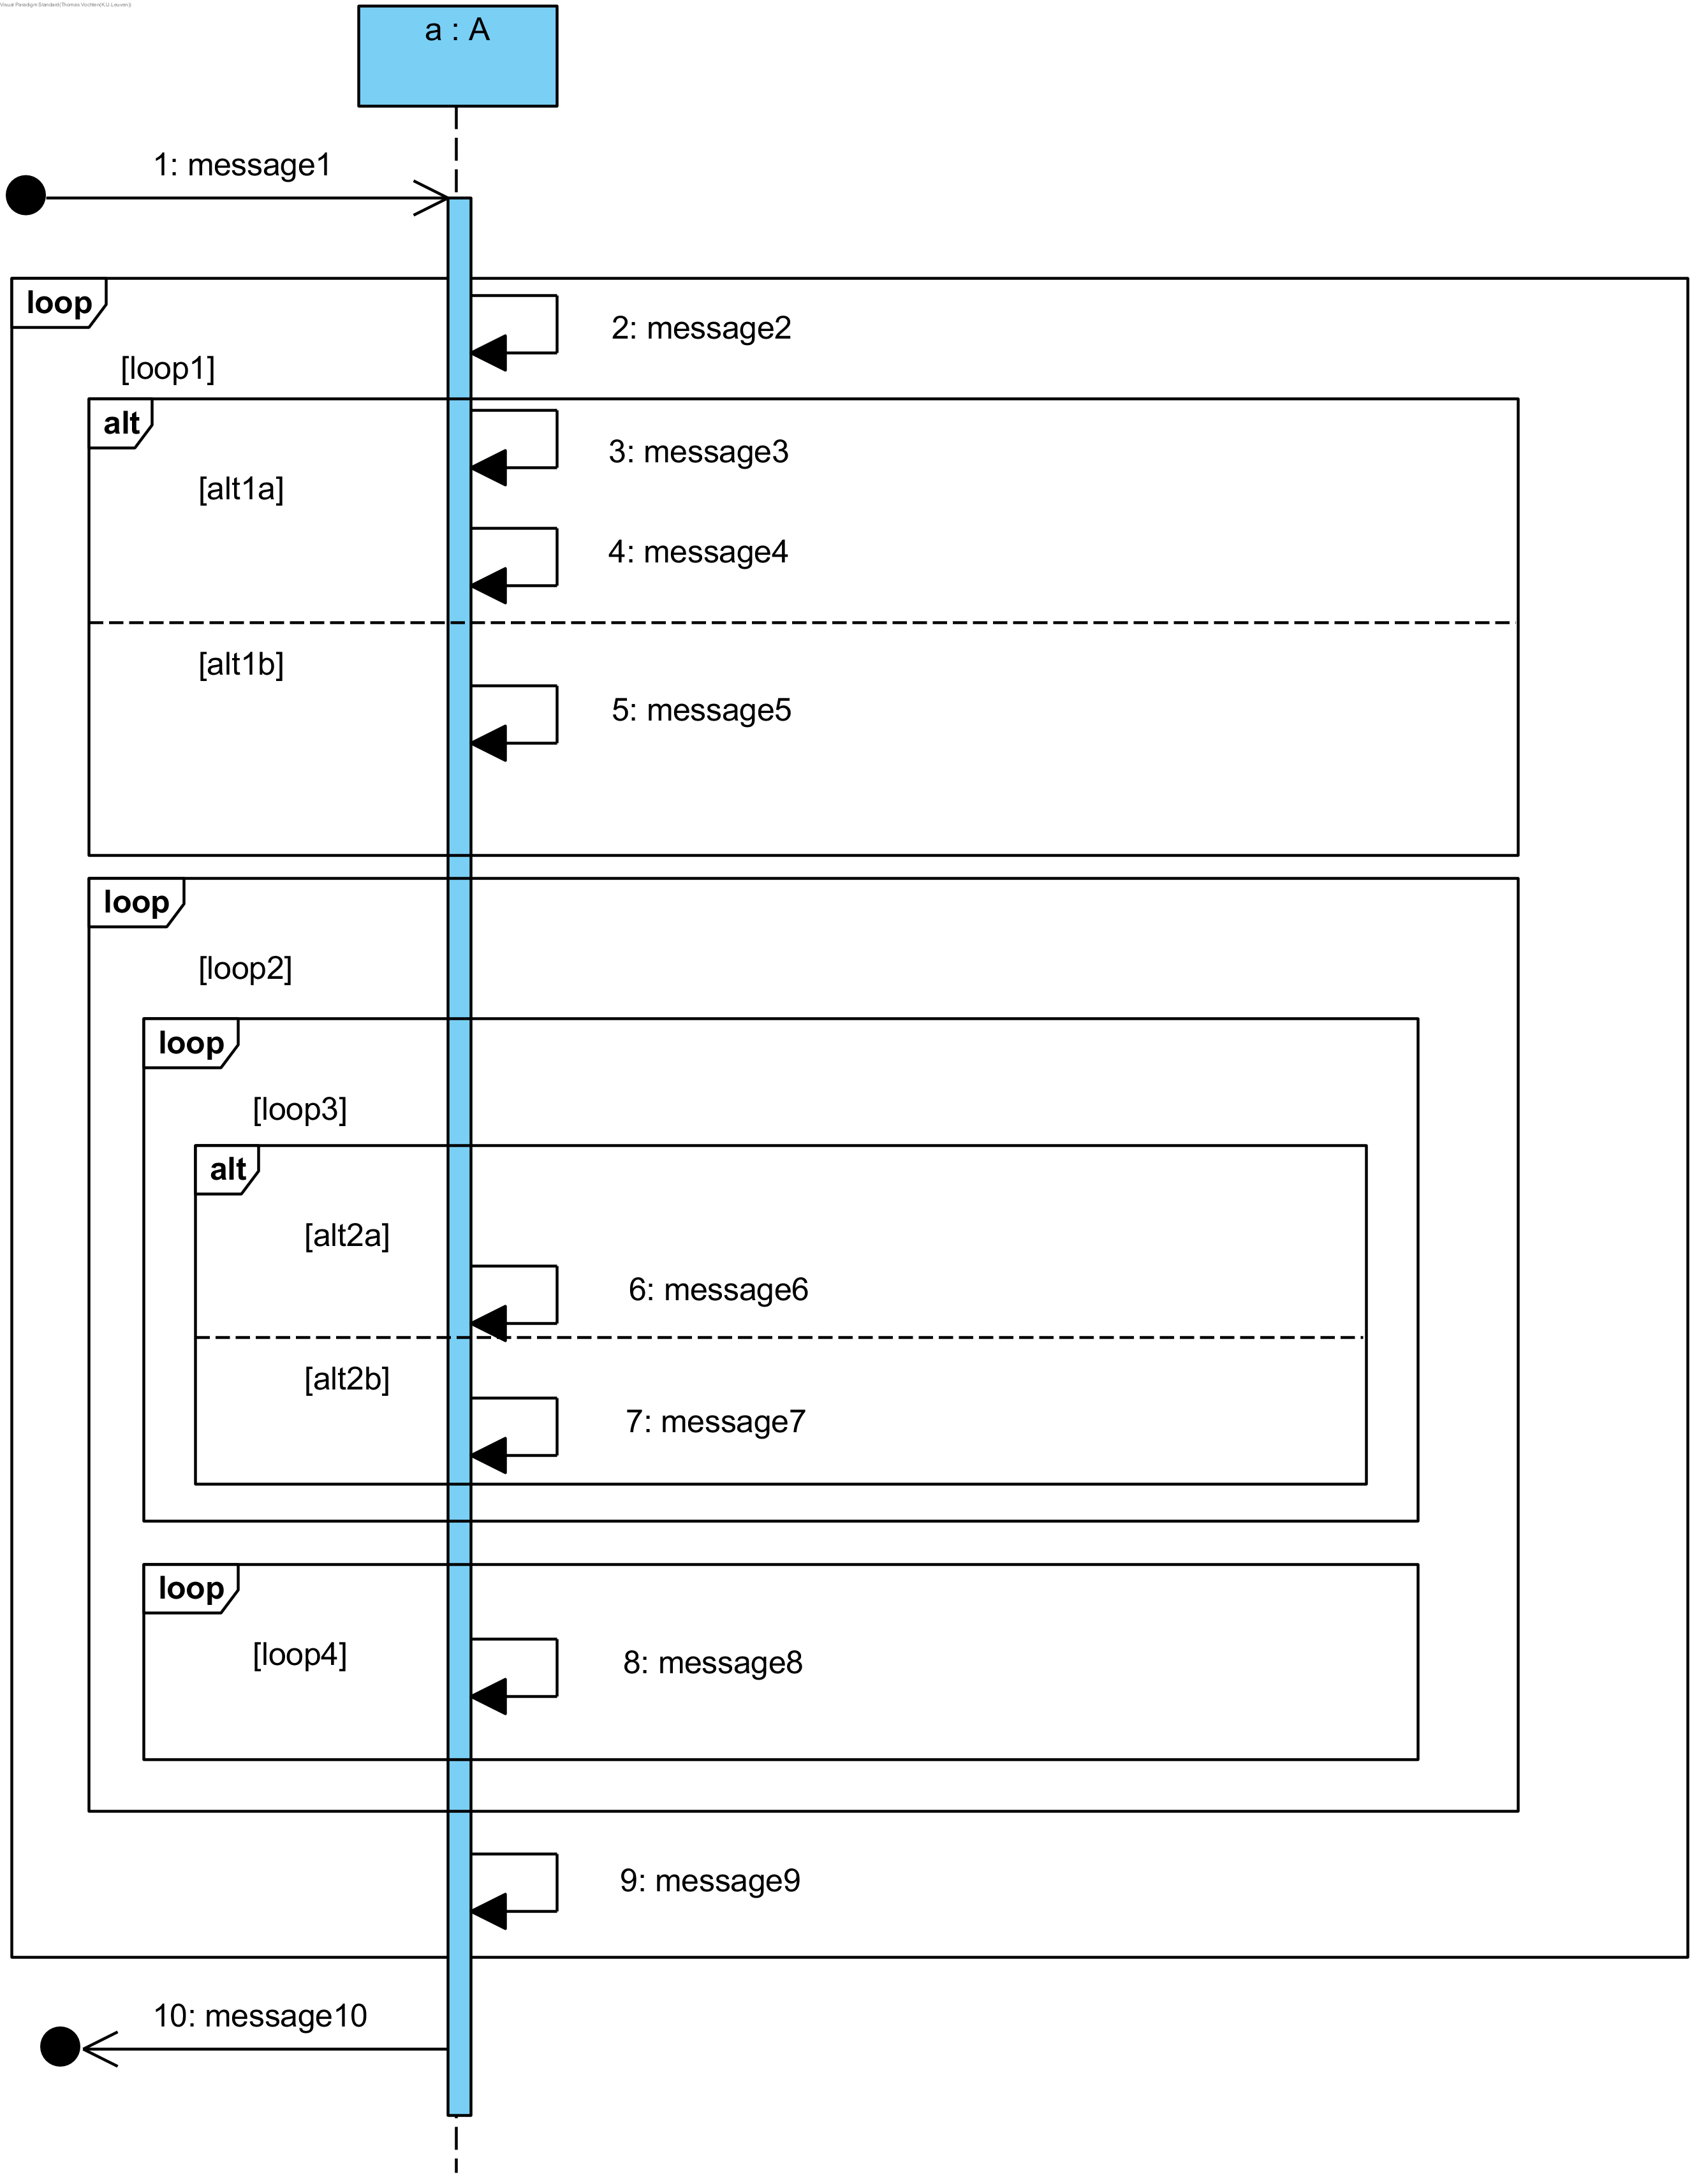
\includegraphics[width=1\textwidth]{chap-gedrag/seq-diagram-frag-ex.png}
	\caption{Sequentiediagram voor een voorbeeldvertaling van gecombineerde fragmenten}
	\label{fig:seq-diagram-frag-ex}
\end{figure}

In wat volgt gebruiken we de voorwaarde voor een fragment als naam voor het fragment zelf. Om het onderscheid te maken tussen deze twee manieren waarop we de voorwaarde gebruiken, schrijven we \fragname{loop1} om aan te duiden dat de voorwaarde als naam wordt gebruikt en \fragcond{loop1} wanneer we het effectief als voorwaarde voor de uitvoering van een fragment gebruiken. \fragname{alt1} verwijst naar het gehele alt-fragment en \fragname{alt1a} en \fragname{alt1b} verwijzen respectievelijk naar het \textit{if}-deel en het \textit{else}-deel.

We roepen algoritme \ref{alg:processCombinedFragment} eerst op op met \fragname{loop1} als argument. Aangezien het geen ouder heeft en \fragmessage{message1}, wat geen fragment heeft, eraan voorafgaat, noteren we in de uitvoer:

\begin{align*}
	&\transitionentry[\fragmessage{message1}]{\lnot \fragcond{loop1}}{\fragmessage{message10}}
\end{align*}

Er is geen fragment dat v\'o\'or dit fragment komt, dus roepen we algoritme \ref{alg:transition-to-frag} op. \fragmessage{message2} is rechtstreeks deel van \fragname{loop1}, dus noteren we in de uitvoer voor dit algoritme:

\begin{align*}
	\transitionentry{\fragcond{loop1}}{\fragmessage{message2}}
\end{align*}

Hierna gaan we verder naar algoritme \ref{alg:wrap-loops} met \fragname{alt1} en \fragname{loop2} als invoerfragmenten en \textit{allemaal} gezet naar \textbf{true}. \fragname{alt1} is geen lusfragment en slaan we over. Vervolgens roepen we algoritme \ref{alg:transition-to-frag} op met \fragname{loop2} als argument.
\fragmessage{message6} is niet rechtstreeks deel van \fragname{loop2}, dus zetten we \textit{voorwaarde} naar \fragcondt{loop2} en roepen eerst algoritme \ref{alg:transition-to-frag} op met \fragname{loop3} als argument. Op dit niveau wordt \textit{voorwaarde} gezet naar ``\fragcond{loop2} $\land$ \fragcond{loop3}'' en roepen we algoritme \ref{alg:transition-to-frag} op met \fragname{alt2} als argument. \fragmessage{message6} en \fragmessage{message7} zijn rechtstreeks deel van \fragname{alt2}, dus hebben we:

\begin{align*}
	&\transitionentry{\fragcond{loop2} \land \fragcond{loop3} \land \fragcond{alt2a}}{\fragmessage{message6}} \\
	&\transitionentry{\fragcond{loop2} \land \fragcond{loop3} \land \fragcond{alt2b}}{\fragmessage{message7}}
\end{align*}

We keren terug naar het niveau van \fragname{loop2}. \fragname{loop3} was een lus, dus zetten we \textit{voorwaarde} naar ``\fragcond{loop2} $\land \lnot$ \fragcond{loop3}'' en roepen we algoritme \ref{alg:wrap-loops} op met als argument de verzameling met enkel \fragname{loop4} als lid. Het resultaat van die oproep is dat we neerschrijven:

\begin{align*}
	\transitionentry{\fragcond{loop2} \land \lnot \fragcond{loop3} \land \fragcond{loop4}}{\fragmessage{message8}}
\end{align*}

We keren terug naar het niveau van \fragname{loop2}. Dit fragment heeft verder geen kinderen, dus eindigt deze oproep van algoritme \ref{alg:wrap-loops} hier.

We keren terug naar stap 7 in algoritme \ref{alg:transition-to-frag} voor \fragname{loop1}. \fragname{alt1} is niet eerder gemarkeerd door algoritme \ref{alg:wrap-loops}, dus gebruiken we het als argument voor een oproep van algoritme \ref{alg:transition-to-frag}. Het resultaat van die oproep is:

\begin{align*}
	&\transitionentry{\fragcond{alt1a}}{\fragmessage{message3}} \\
	&\transitionentry{\fragcond{alt1b}}{\fragmessage{message5}}
\end{align*}

Dit markeert het einde van algoritme \ref{alg:transition-to-frag} voor \fragname{loop1}. In algoritme \ref{alg:processCombinedFragment} gaan we nu over naar stap 10. Na het uitvoeren van de lus verkrijgen we:

\begin{align*}
	&\transitionentry[\fragmessage{message1}]{\fragcond{loop1}}{\fragmessage{message2}} \\
	&\transitionentry[\fragmessage{message2}]{\fragcond{alt1a}}{\fragmessage{message3}} \\
	&\transitionentry[\fragmessage{message2}]{\fragcond{alt1b}}{\fragmessage{message5}} \\
	&\transitionentry[\fragmessage{message4}]{\fragcond{loop2} \land \fragcond{loop3} \land \fragcond{alt2a}}{\fragmessage{message6}} \\
	&\transitionentry[\fragmessage{message5}]{\fragcond{loop2} \land \fragcond{loop3} \land \fragcond{alt2a}}{\fragmessage{message6}} \\
	&\transitionentry[\fragmessage{message4}]{\fragcond{loop2} \land \fragcond{loop3} \land \fragcond{alt2b}}{message7} \\
	&\transitionentry[\fragmessage{message5}]{\fragcond{loop2} \land \fragcond{loop3} \land \fragcond{alt2b}}{message7} \\
	&\transitionentry[\fragmessage{message6}]{\fragcond{loop2} \land \lnot \fragcond{loop3} \land \fragcond{loop4}}{message8} \\
	&\transitionentry[\fragmessage{message7}]{\fragcond{loop2} \land \lnot \fragcond{loop3} \land \fragcond{loop4}}{message8}
\end{align*}

Nu bereiken we stap 18 in algoritme \ref{alg:processCombinedFragment}. Deze stap houdt in dat we algoritme \ref{alg:calcExitForMessages} oproepen met \fragname{loop1} als argument.

In stap 1 roepen we eerst algoritme \ref{alg:determineFinalMessage} op met \fragname{loop1} als argument. De uitkomst daarvan is dat \fragmessage{message9} herkend wordt als laatste bericht. \fragname{loop1} heeft geen ouder, dus gebruiken we algoritme \ref{alg:exitToOutside} met \fragname{loop1} als fragment en ``$\lnot$ \fragcond{loop1}'' als transitievoorwaarde als invoer. Er volgen geen fragmenten op \fragname{loop1} en \fragmessage{message10} is geen deel van een fragment, dus noteren we:

\begin{align*}
	\transitionentry{\lnot \fragcond{loop1}}{\fragmessage{message10}}
\end{align*}

Voor stap 6 in algoritme \ref{alg:calcExitForMessages} noteren we:

\begin{align*}
	\transitionentry[\fragmessage{message9}]{\lnot \fragcond{loop1}}{\fragmessage{message10}}
\end{align*}

Algoritme \ref{alg:calcExitForMessages} gaat nu verder met de kinderen van \fragname{loop1}. \fragname{alt1} komt eerst aan bod, en we bekijken eerst het \textit{if}-deel. Het resultaat van algoritme \ref{alg:determineFinalMessage} is \textit{\{\fragmessage{message4}, $\epsilon$\}}. \fragname{loop1} is de ouder van \fragname{alt1} en \fragmessage{message6} is deel van \fragname{loop1}, dus we gaan naar stap 11. In wat volgt roepen we algoritme \ref{alg:transition-to-frag} op met \fragname{loop2} als argument. Het resultaat daarvan gebruiken we om te noteren:

\begin{align*}
	&\transitionentry[\fragmessage{message4}]{\fragcond{loop2} \land \fragcond{loop3} \land \fragcond{alt2a}}{\fragmessage{message6}} \\
	&\transitionentry[\fragmessage{message4}]{\fragcond{loop2} \land \fragcond{loop3} \land \fragcond{alt2b}}{\fragmessage{message7}} \\
	&\transitionentry[\fragmessage{message4}]{\fragcond{loop2} \land \lnot \fragcond{loop3} \land \fragcond{loop4}}{\fragmessage{message8}}
\end{align*}

Als gevolg van het feit dat \fragmessage{message9} volgt op \fragname{loop2}, noteren we ook:

\begin{align*}
	&\transitionentry[\fragmessage{message4}]{\lnot \fragcond{loop2}}{message9}
\end{align*}

Het voorgaande wordt herhaald voor het \textit{else}-deel. Op gelijkaardige wijze voor het \textit{if}-deel leidt dit tot:

\begin{align*}
	&\transitionentry[\fragmessage{message5}]{\fragcond{loop2} \land \fragcond{loop3} \land \fragcond{alt2a}}{\fragmessage{message6}} \\
	&\transitionentry[\fragmessage{message5}]{\fragcond{loop2} \land \fragcond{loop3} \land \fragcond{alt2b}}{\fragmessage{message7}} \\
	&\transitionentry[\fragmessage{message5}]{\fragcond{loop2} \land \lnot \fragcond{loop3} \land \fragcond{loop4}}{\fragmessage{message8}} \\
	&\transitionentry[\fragmessage{message5}]{\lnot \fragcond{loop2}}{message9}
\end{align*}

We gaan terug naar stap 31 voor \fragname{loop1}. Algoritme \ref{alg:calcExitForMessages} wordt nu opgeroepen op \fragname{loop2}. Via algoritme \ref{alg:determineFinalMessage} concluderen we dat \fragname{loop2} geen laatste bericht heeft, dus roepen we algoritme \ref{alg:calcExitForMessages} op met elk kind om de beurt als argument. \fragname{loop3} komt eerst. Op gelijkaardige wijze gaan we verder naar \fragname{alt2}.

Het \textit{if}-deel van \fragname{alt2} komt eerst. Algoritme \ref{alg:determineFinalMessage} besluit dat \fragmessage{message6} het laatste bericht is. \fragmessage{message8} is geen deel van \fragname{loop3}, dus zetten we \textit{aggregateVoorwaarde} naar ``$\lnot$ \fragcond{loop3}'' en \textit{fragment} naar \fragname{loop2} en gaan naar stap 10. \fragname{message8} is deel van \fragname{loop2}, dus roepen we algoritme \ref{alg:transition-to-frag} op met \fragname{loop4} als argument en concateneren \textit{aggregateVoorwaarde}, wat resulteert in:

\begin{align*}
	\transitionentry[\fragmessage{message6}]{\fragcond{loop4} \land \lnot \fragcond{loop3}}{\fragmessage{message8}}
\end{align*}

\fragname{loop4} is een lus, dus zetten we \textit{fragment} naar \fragname{loop1} en gaan naar stap 10. \fragmessage{message8} is deel van \fragname{loop1}, maar \fragname{loop2} is gemarkeerd in de vorige iteratie en slaan we dus over. We zien wel dat \fragname{loop1} een bericht heeft na \fragmessage{message8}, namelijk \fragmessage{message9}, en daarom noteren we:

\begin{align*}
	\transitionentry[\fragmessage{message6}]{\lnot \fragcond{loop3} \land \lnot \fragcond{loop4} \land \lnot \fragcond{loop2}}{\fragmessage{message9}}
\end{align*}

Met het vinden van dat bericht na \fragmessage{message8}, eindigt het algoritme voor het \textit{if}-deel van \fragname{alt2}. Nu komt het \textit{else}-deel van \fragname{alt2} aan bod, en gelijkaardig voor het \textit{if}-deel krijgen we:

\begin{align*}
		&\transitionentry[\fragmessage{message7}]{\fragcond{loop4} \land \lnot \fragcond{loop3}}{\fragmessage{message8}} \\
		&\transitionentry[\fragmessage{message7}]{\lnot \fragcond{loop3} \land \lnot \fragcond{loop4} \land \lnot \fragcond{loop2}}{\fragmessage{message9}}
\end{align*}

\fragname{loop3} is nu volledig behandeld, en we gaan terug naar stap 31 voor \fragname{loop2}. We roepen algoritme \ref{alg:calcExitForMessages} op met \fragname{loop4} als argument. Algoritme \ref{alg:determineFinalMessage} besluit dat \fragmessage{message8} het laatste bericht is en we zetten \textit{aggregateVoorwaarde} naar ``$\lnot$ \fragcond{loop4}''. \fragname{loop2} heeft geen bericht na \fragmessage{message8}, dus zetten we fragment naar \fragname{loop1} en gaan terug naar stap 8. \fragmessage{message9} komt in \fragname{loop1} meteen na \fragmessage{message8} en is rechtstreeks deels van \fragname{loop1}, dus noteren we:

\begin{align*}
	\transitionentry[\fragmessage{message8}]{\lnot \fragcond{loop4} \land \lnot \fragcond{loop2}}{\fragmessage{message9}}
\end{align*}

Hier stopt de uitvoering van het algoritme voor \fragname{loop4}, en hiermee meteen ook voor \fragname{loop2} en \fragname{loop1}.

\parbreak

We bereiken stap 19 in algoritme \ref{alg:processCombinedFragment}. In plaats van \fragname{loop1} te gebruiken als argument zoals het zou zijn in een echte uitvoering, gebruiken we \fragname{loop4} als illustratiever voorbeeld.

\fragmessage{message8} is vanzelfsprekend het laatste bericht van \fragname{loop4}. We roepen de variant van algoritme \ref{alg:transition-to-frag} gebruikt in dit algoritme op met \fragname{loop4} als argument. De uitkomst van deze iteratie is:

\begin{align*}
	\transitionentry[\fragmessage{message8}]{\fragcond{loop4}}{\fragmessage{message8}}
\end{align*}

We voegen \fragname{loop4} toe aan \textit{uitgesloten} en zetten \textit{aggregateVoorwaarde} naar ``$\lnot$ \fragcond{loop4}'' en \textit{fragment} naar \fragname{loop2}. De laatste container van \fragname{loop2} is een fragment en \fragmessage{message8} is daar het laatste bericht van, dus zetten we \textit{bundelVoorwaarde} naar ``\fragcond{loop2}''. \fragname{loop4} is lid van \textit{uitgesloten}, dus noteren we:

\begin{align*}
	&\transitionentry[\fragmessage{message8}]{\lnot \fragcond{loop4} \land \fragcond{loop2} \land \fragcond{loop3} \land \fragcond{alt2a}}{\fragmessage{message6}} \\
	&\transitionentry[\fragmessage{message8}]{\lnot \fragcond{loop4} \land \fragcond{loop2} \land \fragcond{loop3} \land \fragcond{alt2b}}{\fragmessage{message7}}
\end{align*}

We voegen \fragname{loop2} toe aan \textit{uitgesloten}, concateneren \textit{aggregateVoorwaarde} met ``$\land \lnot$ \fragcond{loop2}'' en gaan verder met \fragname{loop1}. \fragmessage{message8} is geen laatste bericht van \fragname{loop1}, en \fragname{loop1} heeft geen ouder. De uitvoering van algoritme \ref{alg:calculateLoopReentry} stopt.

\parbreak

Nadat we algoritme \ref{alg:processCombinedFragment} hebben uitgevoerd op alle fragmenten, rest de taak van de uitvoer van dat algoritme te vertalen naar logica.

\subsubsection{De uitvoer van de algoritmes vertalen naar logica}

Het is eenvoudig om de uitvoer te vertalen naar logica. We zoeken naar gevallen waar het bericht waarnaar gesprongen wordt en de voorwaarde waaronder die sprong gebeurt overeenkomen en combineren ze. Als voorbeeld:

\begin{align*}
	&\transitionentry[\fragmessage{$message_b$}]{\fragcond{voorwaarde}}{\fragmessage{$message_a$}} \\
	&\transitionentry[\fragmessage{$message_c$}]{\fragcond{voorwaarde}}{\fragmessage{$message_a$}}
\end{align*}

Dit vertalen we naar:

\begin{align*}
	\forall{t}[Time](C\_SDPointAt(Next(t), message_a) \leftarrow (SDPointAt(t, message_b) \\ \lor SDPointAt(t, message_c)) \land \fragcond{voorwaarde}).
\end{align*}

De uitvoer van algoritme \ref{alg:processCombinedFragment} voor alle fragmenten in figuur \ref{fig:seq-diagram-frag-ex} vertalen we op die manier als volgt naar logica:

\begin{align*}
	&\forall{t}[Time](C\_SDPointAt(Next(t), 2) \leftarrow (SDPointAt(t, 1) \\ &\lor SDPointAt(t, 9)) \land \fragcond{loop1}). \\
	&\forall{t}[Time](C\_SDPointAt(Next(t), 3) \leftarrow SDPointAt(t, 2) \\ &\land \fragcond{alt1a}). \\
	&\forall{t}[Time](C\_SDPointAt(Next(t), 5) \leftarrow SDPointAt(t, 2) \\ &\land \fragcond{alt1b}). \\
	&\forall{t}[Time](C\_SDPointAt(Next(t), 6) \leftarrow (SDPointAt(t, 6) \\ &\lor SDPointAt(t, 7)) \land \fragcond{loop3} \land \fragcond{alt2a})). \\
	&\forall{t}[Time](C\_SDPointAt(Next(t), 6) \leftarrow SDPointAt(t, 8) \\ &\land \lnot \fragcond{loop4} \land \fragcond{loop2} \land \fragcond{loop3} \land \fragcond{alt2a}). \\
	&\forall{t}[Time](C\_SDPointAt(Next(t), 6) \leftarrow (SDPointAt(t, 4) \\ &\lor SDPointAt(t, 5)) \land \fragcond{loop2} \land \fragcond{loop3} \land \fragcond{alt2a}). \\
	&\forall{t}[Time](C\_SDPointAt(Next(t), 7) \leftarrow (SDPointAt(t, 6) \\ &\lor SDPointAt(t, 7)) \land \fragcond{loop3} \land \fragcond{alt2b})). \\
	&\forall{t}[Time](C\_SDPointAt(Next(t), 7) \leftarrow SDPointAt(t, 8) \\ &\land \lnot \fragcond{loop4} \land \fragcond{loop2} \land \fragcond{loop3} \land \fragcond{alt2b}). \\
	&\forall{t}[Time](C\_SDPointAt(Next(t), 7) \leftarrow (SDPointAt(t, 4) \\ &\lor SDPointAt(t, 5)) \land \fragcond{loop2} \land \fragcond{loop3} \land \fragcond{alt2b}).
\end{align*}

\begin{align*}
	&\forall{t}[Time](C\_SDPointAt(Next(t), 8) \leftarrow (SDPointAt(t, 6) \\ &\lor SDPointAt(t, 7)) \land \lnot \fragcond{loop3} \land \fragcond{loop4}). \\
	&\forall{t}[Time](C\_SDPointAt(Next(t), 8) \leftarrow (SDPointAt(t, 4) \\ &\lor SDPointAt(t, 5)) \land \fragcond{loop2} \land \lnot \fragcond{loop3} \\ &\land \fragcond{loop4}). \\
	&\forall{t}[Time](C\_SDPointAt(Next(t), 8) \leftarrow SDPointAt(t, 8) \\ &\land \fragcond{loop4}). \\
	&\forall{t}[Time](C\_SDPointAt(Next(t), 9) \leftarrow (SDPointAt(t, 6) \\ &\lor SDPointAt(t, 7)) \land \lnot \fragcond{loop3} \land \lnot \fragcond{loop4} \\ &\land \lnot \fragcond{loop2}). \\
	&\forall{t}[Time](C\_SDPointAt(Next(t), 9) \leftarrow SDPointAt(t, 8) \\ &\land \lnot \fragcond{loop4} \land \lnot \fragcond{loop2}). \\
	&\forall{t}[Time](C\_SDPointAt(Next(t), 9) \leftarrow (SDPointAt(t, 4) \\ &\lor SDPointAt(t, 5)) \land \lnot \fragcond{loop2}). \\
	&\forall{t}[Time](C\_SDPointAt(Next(t), 10) \leftarrow (SDPointAt(t, 1) \\ &\lor SDPointAt(t, 9)) \land \lnot \fragcond{loop1}).
\end{align*}

\section{Interactie tussen meerdere sequentiediagrammen}\label{sec:interaction}
In een project stelt men doorgaans meerdere sequentiediagrammen op die elkaar ook kunnen oproepen. Men gebruikt soms ook recursie in deze diagrammen. In deze sectie beschrijven we hoe we het oproepen van andere sequentiediagrammen en een recursiemechanisme ondersteunen.

\begin{figure}
	\centering
	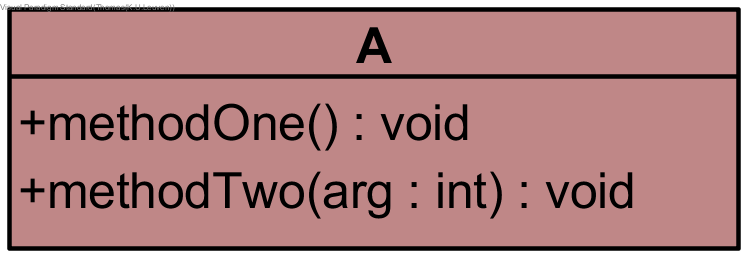
\includegraphics[width=0.25\textwidth]{chap-gedrag/recursion-class.png}
	\caption{Klasse gebruikt in voorbeeld over recursie}
	\label{fig:recursion-class}
\end{figure}

\begin{landscape}
\thispagestyle{empty}
	\begin{figure}
		\centering
		\begin{subfigure}{\textwidth}
			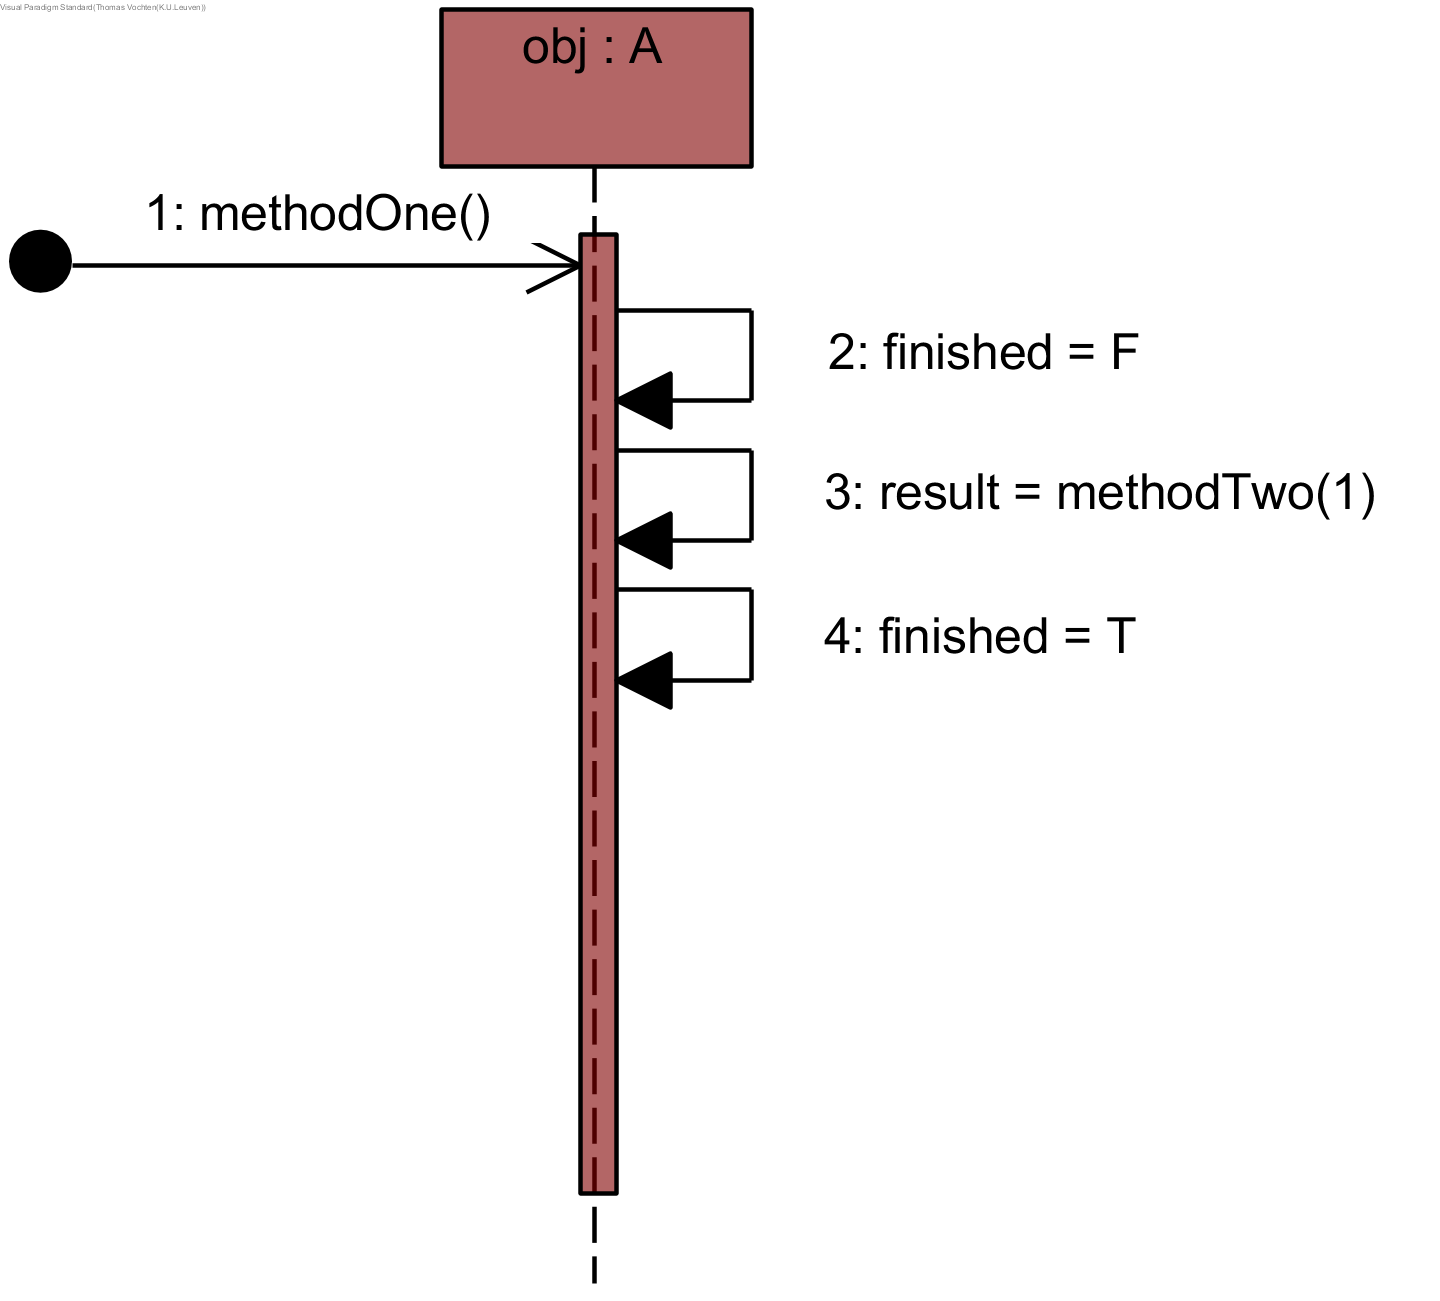
\includegraphics[width=0.4\textwidth]{chap-gedrag/methodOne.png}
			\caption{Sequentiediagram voor methodOne()}
			\label{fig:methodOne}
		\end{subfigure}%
		\begin{subfigure}{\textwidth}
			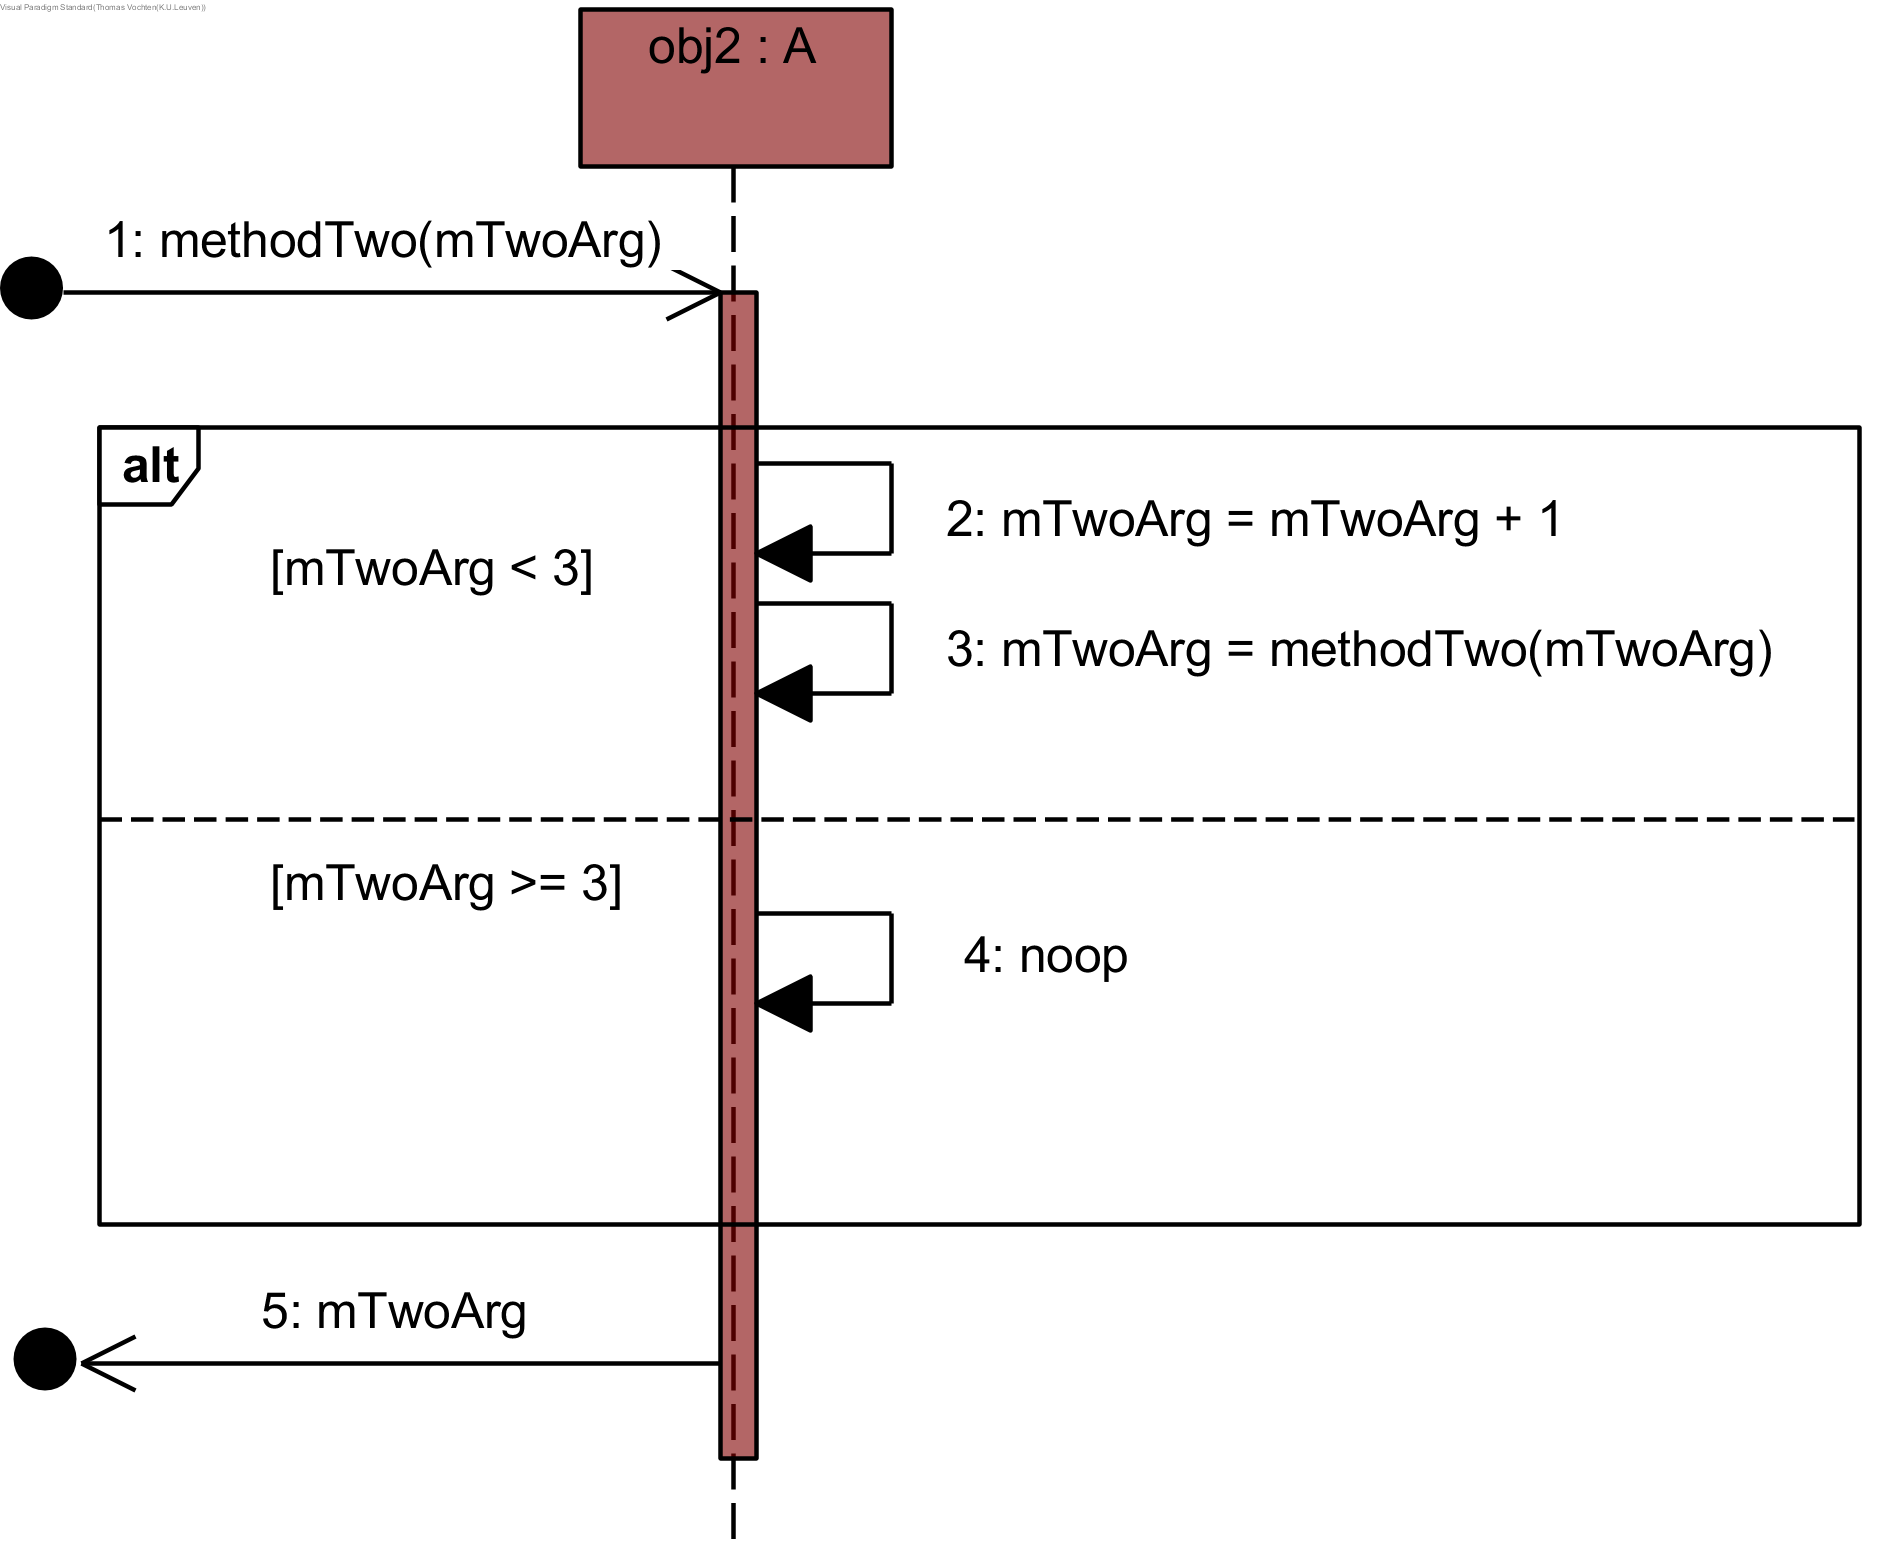
\includegraphics[width=0.75\textwidth]{chap-gedrag/methodTwo.png}
			\caption{Sequentiediagram voor methodTwo()}
			\label{fig:methodtwo}
		\end{subfigure}
		\caption{Sequentiediagrammen voor klasse A in figuur \ref{fig:recursion-class}}
		\label{fig:seq-recursion}
	\end{figure}
\end{landscape}

In de volgende subsecties gebruiken we het voorbeeld uitgebeeld in figuren \ref{fig:recursion-class} en \ref{fig:seq-recursion} om de gebruikte principes te illustreren.

\subsection{Aanpassingen aan \textit{SDPoint}}
Het is niet meer voldoende om \textit{SDPoint}s te modelleren als natuurlijke getallen aangezien elk diagram zijn eigen \textit{SDPoint}s heeft. Om de \textit{SDPoint}s horende bij elk diagram van elkaar te kunnen onderscheiden, maken we van het logisch type \textit{SDPoint} nu een \textit{constructed type} in IDP. We gebruiken als patroon voor de naamgeving van elk logisch object $<diagramnaam>\_<instructienummer>$. Voor het voorbeeld krijgen we o.a. $methodOne\_2$ en $methodTwo\_3$. We voegen ook een nieuwe functie toe aan het vocabularium dat gegeven een \textit{SDPoint} het volgende \textit{SDPoint} teruggeeft, namelijk $NextSD(SDPoint) : SDPoint$.

Een andere aanpassing is dat we een virtuele \textit{SDPoint} inpassen na elke instructie voor een oproep. Het naamgevingspatroon hiervoor is $<diagramnaam>\_<instructienummer>post$. Aangezien de derde instructie in figuur \ref{fig:methodOne} een oproep is, krijgen we $methodOne\_3post$. Met deze toevoeging ontkoppelen we twee zaken die bij een oproep komen kijken: Enerzijds dat het mogelijk is dat het resultaat van een oproep wordt toegekend aan een variabele; en anderzijds dat na een oproep er mogelijks een alt-fragment of lusfragment volgt, en dat het dus v\'o\'or de oproep niet noodzakelijk duidelijk is welke de volgende instructie is na de uitvoering van de oproep. Het zou niet mogelijk zijn om voor deze twee zaken het correcte gedrag te verkrijgen zonder een oproepinstructie op deze manier op te splitsen.

\subsection{Het stapelmechanisme}
Om oproepen van andere sequentiediagrammen correct uit te voeren, moet de theorie bijhouden welke variabelen er bestaan tijdens een bepaalde oproep. Bovendien moet de theorie voor recursieve oproepen ook de waardes van een set variabelen kunnen bewaren v\'o\'or een oproep en die waardes herstellen na een oproep. Hiertoe ontwerpen we een stapelmechanisme. Er gebeuren volgende aanpassingen aan het vocabularium:

\begin{itemize}
	\item Toevoeging van het logisch type $StackLevel \subset \mathbb{N}$: Dit stelt de oproepdiepte van een oproep voor.
	\item Toevoeging van een inerti\"ele functie $CurrentStackLevel(Time) : StackLevel$: De oproepdiepte op een bepaald tijdstip.
	\item Toevoeging van een intertieel predicaaat \\ $ReturnPoint(Time, StackLevel, SDPoint)$: Op een bepaald tijdstip, de \textit{SDPoint} waarnaar de uitvoering moet terugkeren wanneer de laatste instructie voor de gegeven \textit{StackLevel} bereikt is.
	\item Alle diagramvariabelen worden nu gemodelleerd door een ternair predicaat dat nu ook de oproepdiepte in rekening neemt. Voor het voorbeeld krijgen we dus bijvoorbeeld $FinishedT(Time, StackLevel, bool)$.
\end{itemize}

De volgende subsecties beschrijven hoe we in het definitieblok voor de causatiezinnen dit stapelmechanisme gebruiken.

\subsubsection{Causatiezinnen voor \textit{SDPointAt/2}}\label{sec:sd-rec-cause}
Oproepinstructies betekenen bijkomende uitzonderingen op het normale verloop van \textit{SDPoints} naast deze die voortkomen uit alt-- en lusfragmenten. In dit geval zijn $methodOne\_3$, $methodTwo\_3$, $methodOne\_5$, $methodTwo\_5$ en $finished$ de nieuwe uitzonderingen. $methodOne\_5$ en $methodTwo\_5$ zijn ook \textit{SDPoint}s die niet in het diagram terug te vinden zijn, maar die we zelf toevoegen. Dit zijn impliciete terugkeerinstructies die we toevoegen voor diagrammen die \textit{void} als resultaat hebben. $finished$ is een speciale \textit{SDPoint} die het einde van de uitvoering aanduidt. De zin die het normale verloop van \textit{SDPoint}s regelt wordt dus:

\begin{align}
	& \nonumber \forall{t}[Time]\forall{s}[SDPoint](C\_SDPointAt(Next(t), NextSD(s) \leftarrow \\ \nonumber &SDPointAt(t,s) \land \lnot((s = methodOne\_3) \lor (s = methodOne\_5) \\ \nonumber &\lor (s = methodTwo\_1) \lor (s = methodTwo\_3) \lor (s = methodTwo\_3post) \\ &\lor (methodTwo\_4) \lor (methodTwo\_5) \lor (s = finished)).
\end{align}

De uitzonderingen als resultaat van een oproep worden als volgt gemodelleerd:

\begin{align}
	 \forall{t}[Time](C\_SDPointAt(Next(t), methodTwo\_1) \leftarrow SDPointAt(t, methodOne\_3).\label{eq:callOne} \\
	 \forall{t}[Time](C\_SDPointAt(Next(t), methodTwo\_1) \leftarrow SDPointAt(t, methodTwo\_3).\label{eq:callTwo}
\end{align}

Zin \ref{eq:callOne} resulteert uit instructie 3 van het diagram voor \textit{methodOne} en zin \ref{eq:callTwo} resulteert uit instructie 3 van het diagram voor \textit{methodTwo}.

De tweede aanpassing is dat er een terugkeer moet gebeuren wanneer het einde van een sequentiediagram is bereikt. Hiervoor maken we gebruik van $ReturnPoint/3$:

\begin{align}
	&\nonumber \forall{t}[Time]\forall{s}[SDPoint](C\_SDPointAt(Next(t), s) \leftarrow \\ \nonumber &ReturnPoint(t, CurrentStackLevel(t), s) \land (SDPointAt(t, methodOne\_5) \\ &\lor SDPointAt(t, methodTwo\_5))).\label{eq:sd-return}
\end{align}

Deze zin drukt uit dat het terugkeerpunt dat is genoteerd voor deze oproepdiepte wordt genomen als de volgende \textit{SDPoint} wanneer het einde van een sequentiediagram is bereikt, in dit geval $methodOne\_5$ of $methodTwo\_5$. We zetten $finished$ hier niet bij omdat er niets op volgt.

\subsubsection{Causatiezinnen voor \textit{ReturnPoint/3}}
Wanneer de uitvoering een oproep bereikt, willen we voor de nieuwe oproepdiepte dat het terugkeerpunt wordt gezet naar de \textit{SDPoint} direct na de oproepinstructie. Daarmee krijgen we de volgende twee zinnen:

\begin{align}
	\nonumber &\forall{t}[Time]\forall{st}[StackLevel](C\_ReturnPoint(Next(t), st, methodOne\_3post) \\ &\leftarrow (CurrentStackLevel(t) = (st-1)) \land SDPointAt(t, methodOne\_3)). \\
	\nonumber &\forall{t}[Time]\forall{st}[StackLevel](C\_ReturnPoint(Next(t), st, methodTwo\_3post) \\ &\leftarrow (CurrentStackLevel(t) = (st-1)) \land SDPointAt(t, methodTwo\_3)).
\end{align}

We willen ook dat een terugkeerpunt verdwijnt eenmaal dat het wordt gebruikt aan het einde van een diagram. Daarom schrijven we de volgende voorwaarde neer voor het oncausatiepredicaat voor \textit{ReturnPoint/3}:

\begin{align}
 \nonumber &\forall{t}[Time]\forall{st}[StackLevel]\forall{sd}[SDPoint](Cn\_ReturnPoint(Next(t), st, sd) \\ \nonumber &\leftarrow (CurrentStackLevel(t) = st) \land ReturnPoint(t, st, sd) \\ &\land (SDPointAt(t, methodOne\_5) \lor SDPointAt(t, methodTwo\_5))).\label{eq:return-uncauses}
\end{align}

Zinnen \ref{eq:sd-return} en \ref{eq:return-uncauses} samen garanderen dat terugkeerpunten gebruikt worden en verdwijnen wanneer het einde van een diagram is bereikt.

\subsubsection{Causatiezinnen voor \textit{CurrentStackLevel(Time) : StackLevel}}

De oproepdiepte moet toenemen wanneer een oproepinstructie wordt uitgevoerd en afnemen wanneer het einde van een diagram is bereikt. Deze respectievelijke gevallen modelleren we als volgt:

\begin{align}
	\nonumber &\forall{t}[Time]\forall{st}[StackLevel](C\_CurrentStackLevel(Next(t), st) \leftarrow \\ \nonumber &(CurrentStackLevel(t) = (st-1)) \land (SDPointAt(t, methodOne\_3) \\ &\lor SDPointAt(t, methodTwo\_3))). \\
	\nonumber &\forall{t}[Time]\forall{st}[StackLevel](C\_CurrentStackLevel(Next(t), st) \leftarrow \\ \nonumber &(CurrentStackLevel(t) = (st+1)) \land (SDPointAt(t, methodOne\_5) \\ &\lor SDPointAt(t, methodTwo\_5))).
\end{align}

\subsubsection{Causatiezinnen voor oproepobjecten en parameters}
Er komen twee nieuwe soorten variabelen bij: Objecten waarvan een methode wordt opgeroepen en parameters van een methode. In het sequentiediagram voor \textit{methodTwo} is \textit{obj2} de naam van het object dat het eerste bericht ontvangt. Wanneer het diagram voor \textit{methodOne} deze methode oproept, moet \textit{obj2} dus gezet worden naar de juiste waarde, in dit geval \textit{obj} omdat \textit{obj} de methode oproept op zichzelf. Een gelijkaardig geval doet zich voor bij de recursieve oproep in het diagram voor \textit{methodTwo}. Daarom krijgen we de volgende zinnen voor \textit{C\_Obj2T/3}:

\begin{align}
	\nonumber &\forall{t}[Time]\forall{s}[StackLevel]\forall{obj}[A](C\_Obj2T(Next(t), s, obj) \leftarrow
	\\ \nonumber &(CurrentStackLevel(t) = (s-1)) \land SDPointAt(t, methodOne\_3) \\ &\land ObjT(t, (s-1), obj)). \\
	\nonumber &\forall{t}[Time]\forall{s}[StackLevel]\forall{obj}[A](C\_Obj2T(Next(t), s, obj) \leftarrow
	\\ \nonumber &(CurrentStackLevel(t) = (s-1)) \land SDPointAt(t, methodTwo\_3) \\ &\land Obj2T(t, (s-1), obj)).
\end{align}

\textit{mTwoArg} in het diagram voor \textit{methodTwo} is een parameter van \textit{methodTwo} dat ook aangesproken wordt in het diagram zelf. In \textit{methodOne} wordt \textit{mTwoArg} gelijkgesteld aan 1 terwijl in \textit{methodTwo} deze eerst met \'e\'en wordt verhoogd. Daarom krijgen we de drie volgende zinnen:

\begin{align}
	\nonumber &\forall{t}[Time]\forall{s}[StackLevel](C\_MTwoArgT(Next(t), s, 1) \leftarrow \\ &(CurrentStackLevel(t) = (s-1)) \land SDPointAt(t, methodOne\_3)). \\
	\nonumber &\forall{t}[Time]\forall{s}[StackLevel]\forall{n}[int](C\_MTwoArgT(Next(t), s, n) \leftarrow \\ \nonumber &(CurrentStackLevel(t) = (s-1)) \land SDPointAt(t, methodTwo\_3) \\ &\land MTwoArg(t, (s-1), n)). \\
	\nonumber &\forall{t}[Time]\forall{s}[StackLevel]\forall{n}[int](C\_MTwoArgT(Next(t), s, n) \leftarrow \\ \nonumber &(CurrentStackLevel(t) = s) \land SDPointAt(t, methodTwo\_2) \\ &\land (\exists{n1}[int](MTwoArg(t, s, n1) \land (n = n1 + 1)))).\label{eq:mtwoarg-inc}
\end{align}

Zin \ref{eq:mtwoarg-inc} demonstreert dat ook buiten oproepinstructies of een terugkeer uit een diagram wordt gekeken naar het oproepniveau. Er wordt immers enkel gekeken of geschreven naar de waarde van de 'versie' van de variabele die overeenkomt met het huidige oproepniveau. Dit komt ook terug bij de variabelen die niet het oproepobject of een parameter van een methode voorstellen.

\subsubsection{Uitkomst van de beschreven procedure}
Er zijn geen noemenswaardige veranderingen aan hoe we de toestandszinnen opstellen. Bijlage \ref{app:seq-recursion} bevat de uitkomst van de procedure die we hebben beschreven in deze sectie. 

\section{Extra veronderstellingen over het ontwerp van sequentiediagrammen}\label{sec:beperkingen}
Om de implementatie van theoriegeneratie zoals beschreven in dit hoofdstuk te vergemakkelijken, zijn er een aantal veronderstellingen ten aanzien van sequentiediagrammen die de gebruiker als invoer geeft. In deze subsectie sommen we deze op:

\begin{itemize}
	\item Er wordt een logisch symbool voorzien voor elke variabele in een sequentiediagram. De naam van dat logisch symbool is gebaseerd op de naam van de variabele, en daarom moeten alle variabelen over alle diagrammen heen een unieke naam hebben. De naam van het diagram waarin de variabele voorkomt kan dienen als prefix om de naam van de variabele toch uniek te maken zonder dat tussenkomst van de ontwerper nodig is. Door tijdsgebrek is dit echter niet ge\"implementeerd.
	\item Het type van een variabele kan niet veranderen over instructies heen. Ofwel komt een variabele overeen met een levenslijn en wordt het type dus bepaald door de levenslijn, ofwel wordt het type bepaald door de instructie die de variabele instantieert.
	\item Een variabele kan geen verzameling voorstellen.
	\item Per instructie kan maar \'e\'en associatielink tegelijkertijd genavigeerd worden. Beschouw het voorbeelddiagram van figuur \ref{fig:diagram-voorbeeld}. Als variabele \textit{x} een object van klasse \textit{Item} is, dan zal een oproep van \textit{getInventory()} op \textit{x} een object van klasse \textit{Inventory} opleveren (mocht die associatie zijn ingevuld voor \textit{x}), maar is \textit{getInventory().getCharacter()} geen geldige instructie.
	\item Er mogen geen aanpassingen worden aangebracht aan de associatiestructuur voor een model van een klassediagram. Voor een \textit{Character}---\textit{Inventory}-paar geldt bijvoorbeeld dat die verbinding niet verbroken kan worden en dat geen van beide kanten vervangen mag worden door een andere instantie van de respectievelijke klasse. Aangezien associaties van meervoudige multipliciteit als lijsten worden ge\"implementeerd, betekent dit ook dat men geen elementen kan toevoegen aan of verwijderen uit een lijst.
	\item Men kan geen nieuwe objecten instanti\"eren.
	\item Er zijn geen bewerkingen op booleaanse waarden behalve de NOT-functie, die men kan oproepen als \textit{flipBool(boolean)}.
	\item UML legt op dat men voor beide takken van een alt-fragment de voorwaarde voor de uitvoering die tak moet specificeren. Ook hier wordt verwacht dat de ontwerper dit telkens doet.
	\item Als een diagram een uitvoer heeft, dan mag de instructie die bepaalt welke variabele als uitvoer wordt gebruikt geen onderdeel zijn van een gecombineerd fragment.
	\item In een fragmentvoorwaarde of een oproep gebeurt er voor de gebruikte waardes geen evaluatie tenzij om de waarde van een variabele op te halen. \textit{call(1 + 2)} en \textit{call(var1 + var2)} worden bijvoorbeeld niet correct vertaald, maar \textit{call(3)} en \textit{call(var1)} wel.
\end{itemize}

\section{Extra soorten instructies voor sequentiediagrammen}\label{sec:newlang}
UML is een modelleertaal die wordt gebruikt ter ondersteuning van softwareontwerp in imperatieve programmeertalen. In sequentiediagrammen vertaalt zich dat tot een veelvoud aan instructies voor eenvoudige taken zoals het selecteren van het eerste getal verschillend van 0 in een lijst van getallen. Aangezien elke nieuwe instructie in een sequentiediagram leidt tot minstens \'e\'en zin in de gegenereerde theorie, impliceert dit een grote kost in zowel rekentijd als geheugengebruik voor modelexpansie en progressie\"inferentie. Daarom geven we in deze sectie een aanzet tot het integreren van logica in het ontwerp van sequentiediagrammen met het zicht op twee doelen:

\begin{enumerate}
	\item Het totale aantal instructies over alle sequentiediagrammen verminderen
	\item Het aantal tijdstappen die nodig zijn bij modelexpansie of progressie\"inferentie om een bepaalde taak te verrichten verminderen
\end{enumerate}

We houden vast aan de structuur van klasses, associaties, levenslijnen en berichten. Wat volgt is een overzicht van nieuwe soorten instructies die gebruikt kunnen worden in berichten.

\subsection{Nieuwe soorten instructies}

Voorheen kon een variabele maar \'e\'en object of waarde van een primitief type voorstellen. Nu laten we toe dat een variabele een verzameling kan voorstellen. In een sequentiediagram wordt dit voorgesteld als een multi-object zoals in figuur \ref{fig:multi-object}. In de theorie behouden we voor namen het patroon $<variabelenaam>T/3$.

We laten op variabelen die een verzameling voorstellen enkele nieuwe instructies toe:

\begin{figure}
	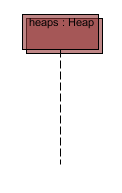
\includegraphics{chap-gedrag/seq-multi-object.png}
	\centering
	\caption{Een multi-object}
	\label{fig:multi-object}
\end{figure}

\begin{itemize}
	\item Voor alle leden van een verzameling tegelijkertijd kan een associatie genavigeerd worden. Als op een verzameling S van objecten van klasse X \textit{getY()} wordt uitgevoerd waar Y de naam is van een klasse geassocieerd met X, dan is het resultaat een verzameling van objecten van klasse Y. Die verzameling bestaat uit alle objecten die in verband staan met minstens \'e\'en object uit S.
	\item $getNumX()$ waar X de naam is van een klasse die in verband staat met de klasse van de verzameling. Het resultaat is de som van het aantal instanties van klasse X waarmee elk lid van de verzameling in verband staat.
	\item $EXISTS\ ONE\ WHERE\ [query]$: Geeft \textbf{true} als en slechts als \textit{query} geldt voor minstens \'e\'en lid van de verzameling. \textit{query} betekent hier een instructie die bestaat uit getters van klassevariabelen verbonden met booleaanse connectieven (klassevariabelen kunnen hierbij rechtstreeks vergeleken worden met een getal of string, waar toepasselijk).
	\item $EXISTS\ n\ TO\ m\ WHERE\ [query]$ waar $n \leq m$: Geeft \textbf{true} als en slechts als voor minstens $n$ en ten hoogste $m$ leden van de verzameling geldt dat \textit{query} waar is.
	\item $FOR\ ALL\ APPLIES\ [query]$: Geeft \textbf{true} als en slechts als voor alle leden van de verzameling \textit{query} geldt.
	\item $NOT\ [query]$: geeft \textbf{true} als en slechts als \textit{query} \textbf{false} geeft. \textit{query} kan hier \'e\'en van de voorgaande soorten instructies zijn.
	\item $CHOOSE\ ALL\ WHERE\ APPLIES\ [query]$: Geeft een nieuwe verzameling die bestaat uit alle leden van de originele verzameling waarvoor \textit{query} waar is.
	\item $CHOOSE\ ONE\ WHERE\ APPLIES\ [query]$: Geeft \'e\'en object uit de verzameling waarvoor \textit{query} waar is. Dit vormt een keuzepunt bij simulatie.
	\item $CHOOSE\ n\ TO\ m\ WHERE\ APPLIES\ [query]$ waar $n \leq m$: Geeft een nieuwe verzameling die bestaat uit minstens $n$ en ten hoogste $m$ leden uit de originele verzameling waarvoor \textit{query} waar is. Dit vormt een keuzepunt bij simulatie.
	\item $CHOOSE\ <getalnaam>\ WHERE\ APPLIES\ [query\ dat\ <getalnaam>\ bindt]$: Geeft een nieuwe variabele met als naam \textit{getalnaam} waarvoor geldt dat de waarde voldoet aan \textit{query}. Dit soort instructie kan ook toegepast worden op een variabele dat maar \'e\'en object voorstelt. Dit vormt een keuzepunt bij simulatie.
	\item $SET <klassevariabele> TO <waarde>$: Voor alle leden van de verzameling wordt de waarde van de genoemde klassevariabele veranderd naar de genoemde waarde.
\end{itemize}

We illustreren het gebruik van deze nieuwe instructies door middel van het voorbeeld van figuur \ref{fig:new-nim}, dat een modellering van het bekende spel Nim voorstelt. De beurt gaat eerst aan de gekozen speler. Dan wordt gecontroleerd of alle stapels leeg zijn. Als dat niet het geval is, kiest de speler eerst een stapel en neemt dan minstens \'e\'en object weg van die stapel. Daarna wordt de beurt gegeven aan de volgende speler. Als alle stapels leeg zijn, is de huidige speler de winnaar. Dit stelt dus een versie van Nim voor waar de speler die als laatste een object wegneemt verliest.

\begin{figure}[H]
	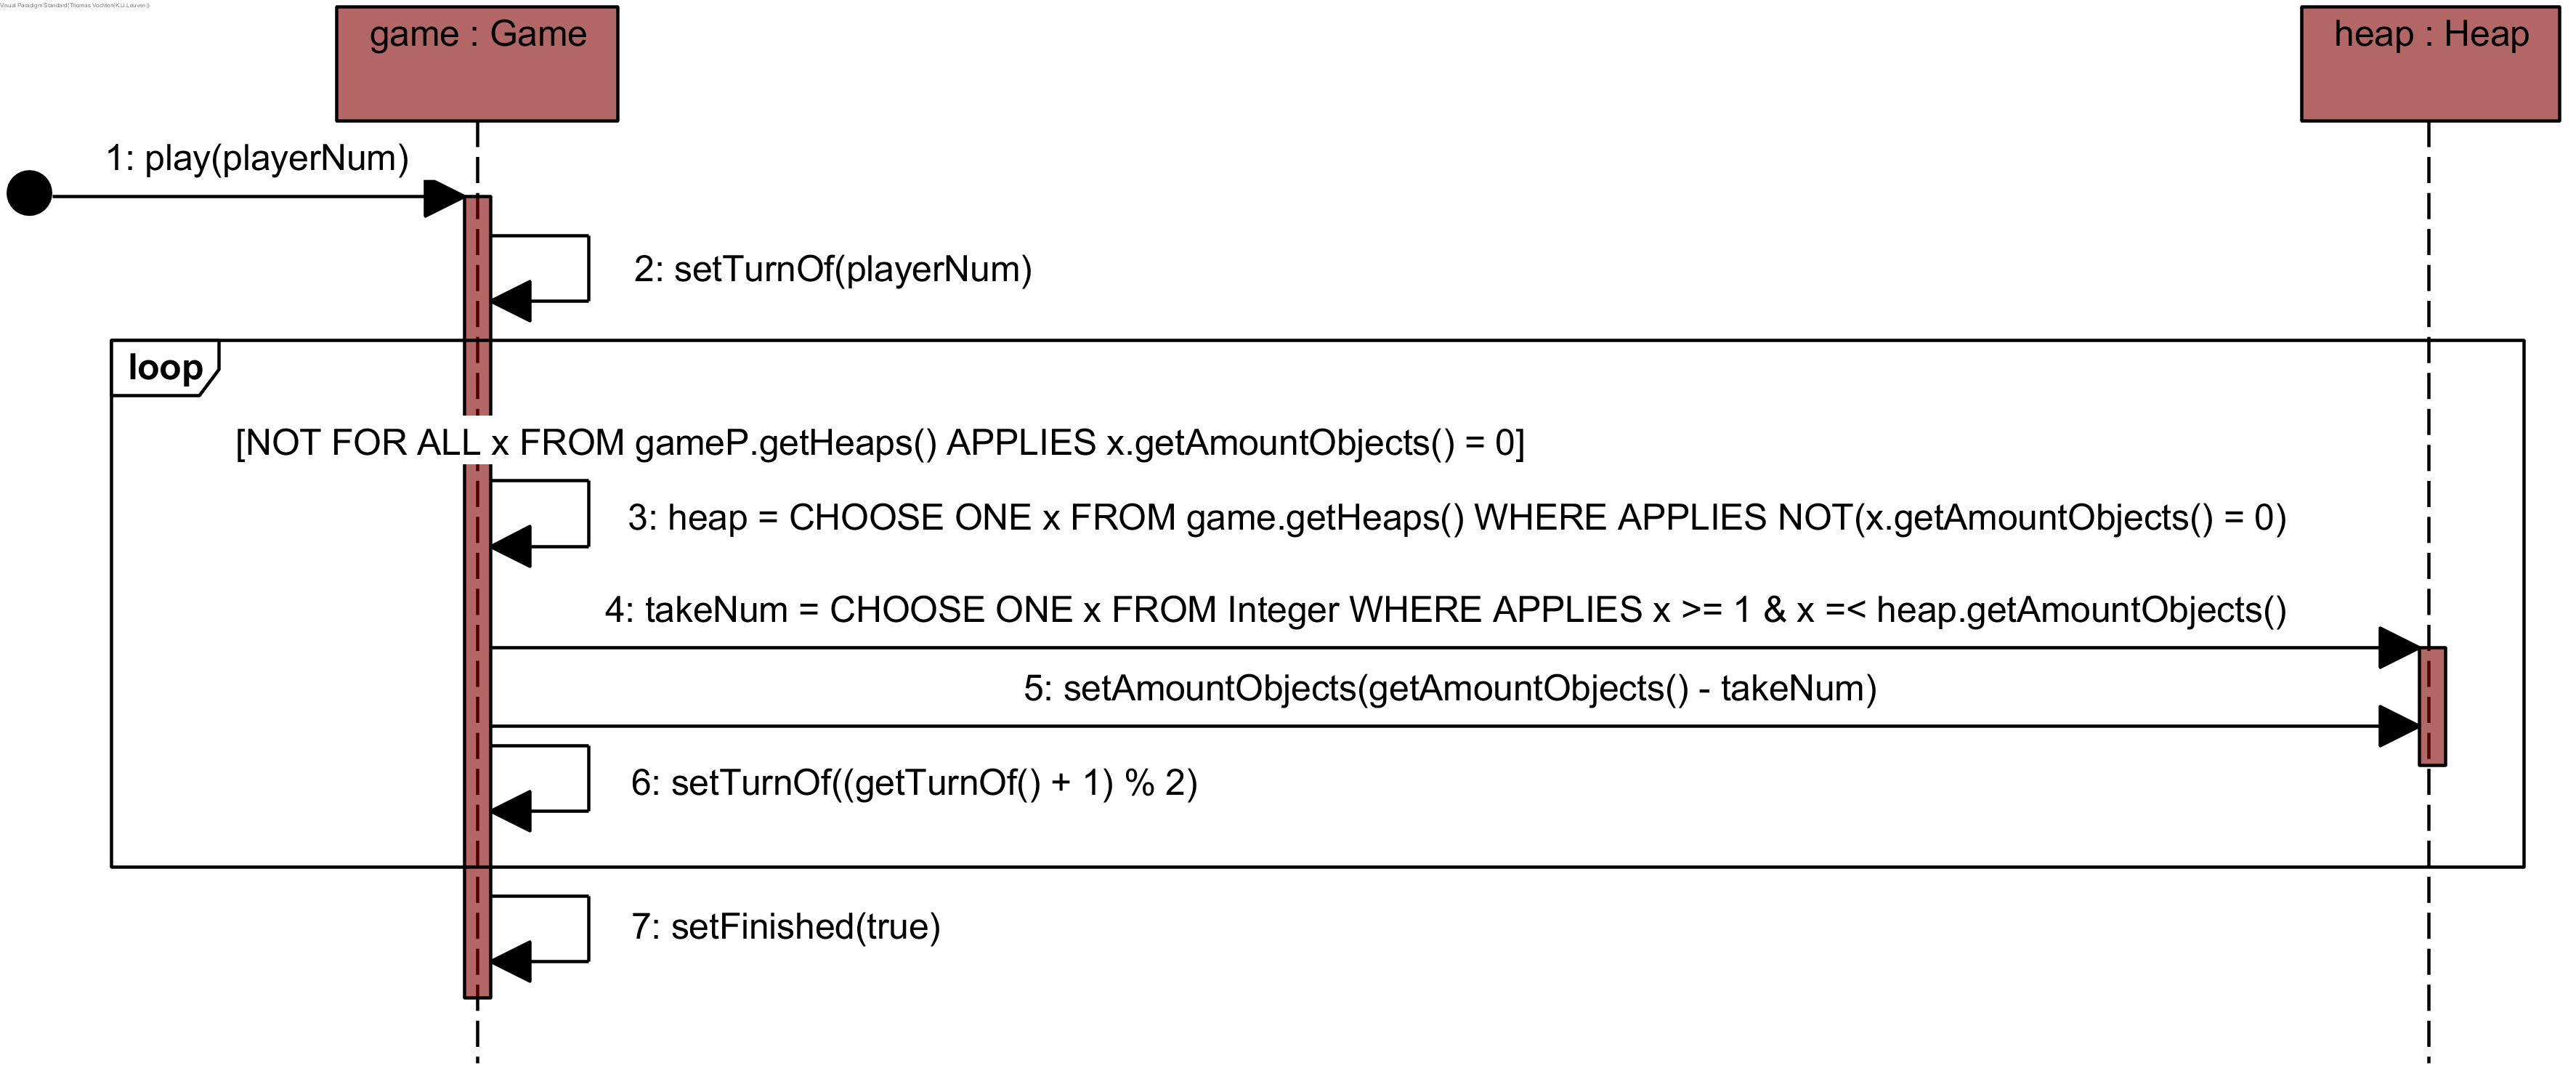
\includegraphics[width=\textwidth]{chap-gedrag/seq-new-nim.png}
	\caption{Een modellering van het spel Nim}
	\label{fig:new-nim}
\end{figure}

De lusvoorwaarde wordt als volgt gebruikt:

\begin{align}
	\nonumber &\forall{t}[Time]\forall{st}[StackLevel](C\_SDPointAt(Next(t), play\_3) \leftarrow \\ \nonumber &(CurrentStackLevel(t) = st) \land (SDPointAt(t, play\_2) \lor SDPointAt(t, play\_6)) \land \\ \nonumber &\lnot{}\exists{g}[Game](GameT(t, st, g) \land{}\forall{h}[Heap](GameandHeap(g, h) \\ &\Rightarrow \exists{n}[LimitedInt](HeapamountObjects(t, h, n) \land n = 0)))). \\
	\nonumber &\forall{t}[Time]\forall{st}[StackLevel](C\_SDPointAt(Next(t), play\_7) \leftarrow \\ \nonumber &(CurrentStackLevel(t) = st) \land SDPointAt(t, play\_6) \land \exists{g}[Game](GameT(t, st, g) \land \\ \nonumber &\forall{h}[Heap](GameandHeap(g, h) \\ &\Rightarrow \exists{n}[LimitedInt](HeapamountObjects(t, h, n) \land n = 0)))).
\end{align}

In instructie 3 wordt de $CHOOSE\ ONE\ WHERE\ APPLIES\ [query]$ instructie gebruikt. We introduceren hier een open predicaat, $ChosenHeap(Time, Heap)$, om ons te helpen deze instructie te vertalen. We voegen de volgende zin toe aan het definitieblok voor diagramvariabelen:

\begin{align}
	\nonumber &\forall{t}[Time]\forall{st}[StackLevel]\forall{h}[Heap](C\_HeapT(Next(t), st, h) \\ &\leftarrow (CurrentStackLevel(t) = st) \land SDPointAt(t, play\_3) \land ChosenHeap(t, h)).
\end{align}

Om ervoor te zorgen dat exact \'e\'en Heap-object wordt gekozen, moeten we voorwaardes leggen op $ChosenHeap/2$. Dit doen we als volgt:

\begin{align}
	&\forall{t}[Time](SDPointAt(t, play\_3) \Rightarrow \exists_{=1}{h}[Heap](ChosenHeap(t, h))).\label{form:uniqueheap} \\
	\nonumber &\forall{t}[Time]\forall{h}[Heap](ChosenHeap(t, h) \Rightarrow (SDPointAt(t, play\_3) \\ \nonumber &\land \exists{g}[Game]\exists{st}[StackLevel]\exists{n}[LimitedInt]((CurrentStackLevel(t) = st) \\ &\land GameT(t, st, g) \land GameandHeap(g, h) \land HeapamountObjects(t, h, n) \land \lnot(n = 0)))).\label{form:correctsd}
\end{align}

Zin \ref{form:uniqueheap} garandeert dat er maar \'e\'en \textit{Heap}-object mag gekozen worden.

Zin \ref{form:correctsd} garandeert dat er enkel een keuze mag gemaakt worden als de uitvoering instructie 3 bereikt en dat er enkel een \textit{Heap}-object wordt gekozen waarvoor geldt dat \textit{amountObjects} groter is dan 0.

Voor instructie 4 introduceren we op een soortgelijke manier een open predicaat $ChosenTake/2$. De zin die we toevoegen aan het definitieblok voor variabelen en de voorwaarden die we opleggen op $ChosenTake/2$ zien er gelijkaardig uit.

Bijlage \ref{code:new-nim} bevat de vertaling van het diagram in figuur \ref{fig:new-nim}.

\appendixpage*
\appendix
\chapter{IDP-bestand voor sequentiediagram van het spelvoorbeeld}\label{app:seq-diagram-game}

\lstinputlisting[title=Modellering van het gedrag van het sequentiediagram in figuur \ref{fig:seq-diagram-game}]{idp-sources/seq-diagram-game.idp}\label{code:seq-diagram-game}

\backmatter

\bibliography{citations}{}
\bibliographystyle{plain}

\end{document}